\documentclass[12pt,a4paper]{report}

% ===========================
% PRÉAMBULE - Packages et configuration
% ===========================

% Encodage et langue
\usepackage[utf8]{inputenc}
\usepackage[french]{babel}
\usepackage[T1]{fontenc}

% Police Times New Roman (conforme aux exigences VAE)
\usepackage{mathptmx} % Times pour le texte et les maths
\usepackage[scaled=.90]{helvet} % Helvetica pour sans-serif

\usepackage{courier} % Courier pour monospace

% Packages mathématiques
\usepackage{amsmath}
\usepackage{amssymb}
\usepackage{amsfonts}

% Citations et guillemets français
\usepackage{csquotes}

% Mise en page
\usepackage{geometry}
\geometry{top=2.5cm, bottom=2.5cm, left=2.5cm, right=2.5cm}

% Correction de la hauteur d'en-tête pour fancyhdr
\setlength{\headheight}{14.5pt}

% Graphiques et images
\usepackage{graphicx}
\usepackage{tikz}
\usetikzlibrary{arrows,shapes,positioning}

% Hyperliens
\usepackage[pdfencoding=auto, psdextra, bookmarks=false]{hyperref}
\hypersetup{
    colorlinks=true,
    linkcolor=blue,
    filecolor=magenta,      
    urlcolor=cyan,
    citecolor=green,
    pdftitle={Dossier VAE Master MEEF PIF - Steeve PYTEL},
    pdfauthor={Steeve PYTEL},
    pdfsubject={Validation des Acquis de l'Expérience},
    pdfkeywords={VAE, MEEF, PIF, Ingénierie, Formation}
}

% En-têtes et pieds de page
\usepackage{fancyhdr}
\pagestyle{fancy}
\fancyhf{}
\fancyhead[L]{Steeve PYTEL}
\fancyhead[R]{Master MEEF PIF}
\fancyfoot[C]{\thepage}

% Titres et sections
\usepackage{titlesec}
\titleformat{\chapter}[display]
  {\normalfont\huge\bfseries}{\chaptertitlename\ \thechapter}{20pt}{\Huge}
\titlespacing*{\chapter}{0pt}{-30pt}{40pt}

% Table des matières
\usepackage{tocloft}
\setcounter{tocdepth}{1}
\setcounter{secnumdepth}{1}

% Tableaux
\usepackage{longtable}
\usepackage{array}
\usepackage{booktabs}
\usepackage{colortbl}
\usepackage{multirow}

% Couleurs
\usepackage{xcolor}
\definecolor{headercolor}{RGB}{0,51,102}
\definecolor{lightgray}{RGB}{240,240,240}

% Listes
\usepackage{enumitem}

% Mode paysage pour tableaux larges
\usepackage{pdflscape}

% Package float pour contrôle placement tableaux
\usepackage{float}

% Citations et bibliographie
\usepackage[backend=biber,style=apa]{biblatex}
\usepackage{tcolorbox}
% \DeclareLanguageMapping{french}{french-apa}
\addbibresource{VAE-MEEF-Bibliographie.bib}

% Index
\usepackage{makeidx}
\makeindex

% Espacements et paragraphes
\usepackage{setspace}
\onehalfspacing

% Commandes personnalisées
\newcommand{\partie}[1]{\part{#1}}
\newcommand{\emphasize}[1]{\textbf{\textit{#1}}}

% ===========================
% DÉBUT DU DOCUMENT
% ===========================

\begin{document}
\pagenumbering{roman}

% ===========================
% PAGE DE TITRE
% ===========================

\begin{titlepage}
    \centering
    
    % Logo 1 en haut de page
    
\includegraphics[height=3cm]{sources/medias/logo1.png}
    
    \vspace{1.5cm}
    
    {\Huge\bfseries Validation des acquis de l'expérience\par}
    \vspace{0.5cm}
    {\huge\bfseries Dossier de Validation\par}
    
    \vspace{2cm}
    
    {\LARGE Master MEEF\par}
    {\LARGE Métiers de l'Enseignement, de l'Éducation et de la Formation\par}
    \vspace{0.5cm}
    {\Large\textbf{Mention Pratiques et Ingénierie de la Formation}\par}
    
    \vspace{2.5cm}
    
    {\Large\textbf{DOSSIER DE M. Steeve PYTEL}\par}
    \vspace{0.5cm}
    {\large Année universitaire 2026-2027\par}
    
    \vfill
    
    % Logo 2 en bas de page remplaçant les informations institutionnelles
    
\includegraphics[height=3cm]{sources/medias/logo2.png}
    
\end{titlepage}

% ===========================
% TABLE DES MATIÈRES
% ===========================

\setcounter{tocdepth}{1} % Limiter la table des matières à 2 niveaux (chapitre + section)
\tableofcontents
\newpage

% ===========================
% PAGES ADMINISTRATIVES
% ===========================

\chapter*{Informations personnelles}
\addcontentsline{toc}{chapter}{Informations personnelles}

\begin{tcolorbox}[colback=white,colframe=headercolor,title=\textbf{CANDIDAT},fonttitle=\large\bfseries]
    \begin{minipage}[c]{0.7\textwidth}
        \textbf{Civilité :} Monsieur\\
        \textbf{Nom :} PYTEL\\
        \textbf{Prénom :} Steeve\\
        \textbf{Date de naissance :} 27/04/1978 (Harfleur 076)\\
        \textbf{Adresse :} 80 avenue du 8 mai 1945, 76610 Le Havre\\
        \textbf{Tél :} 07.70.05.26.46\\
        \textbf{E-mail :} steeve.pytel@univ-lehavre.fr
    \end{minipage}
    \hfill
    \begin{minipage}[c]{0.25\textwidth}
        \centering
        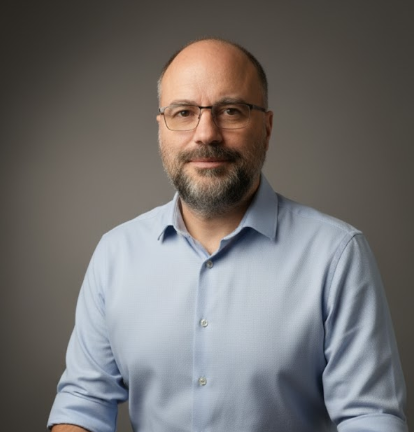
\includegraphics[width=0.9\textwidth,keepaspectratio]{sources/medias/photo.png}
    \end{minipage}
\end{tcolorbox}

\vspace{1cm}

\begin{tcolorbox}[colback=lightgray!30,colframe=gray,title=\textbf{ENCADREMENT},fonttitle=\large\bfseries]
    \textbf{ACCOMPAGNATEUR VAE :} Élisabeth SCHNEIDER\\
    \textit{Maîtresse de Conférences en Information Communication}\\
    Unicaen - Normandie Université - ESO UMR 6590\\
    Chercheure associée au CIRNEF\\
    INSPÉ de Normandie Caen\\
    
    \vspace{0.5cm}
    \textbf{ENSEIGNANT RÉFÉRENT :} Élisabeth SCHNEIDER
\end{tcolorbox}

\newpage

% ===========================
% DÉCLARATION SUR L'HONNEUR
% ===========================

\chapter*{Déclaration sur l'honneur}
\addcontentsline{toc}{chapter}{Déclaration sur l'honneur}

Je soussigné, Monsieur Steeve PYTEL, déclare sur l'honneur :

\begin{itemize}[leftmargin=*]
    \item ne pas faire l'objet d'une mesure pénale ou administrative d'interdiction de présentation devant un jury d'examen ou de validation des acquis de l'expérience
    \item que toutes les informations fournies sont sincères et véritables
    \item que la présente demande de VAE constitue l'unique demande pour ce diplôme durant cette année civile
\end{itemize}

De même, je déclare être pleinement conscient que le plagiat de documents ou d'une partie d'un document publiés sur toutes formes de support, y compris l'internet, constitue une violation des droits d'auteur ainsi qu'une fraude caractérisée. En conséquence, je m'engage à citer toutes les sources que j'ai utilisées pour écrire ce dossier VAE.

\vspace{2cm}

Fait à Le Havre, le \today

\vspace{1.5cm}

Signature

\vspace{2cm}



\newpage

% ===========================
% AUTORISATION DE CONSULTATION
% ===========================

\chapter*{Autorisation de mise en consultation du dossier de VAE}
\addcontentsline{toc}{chapter}{Autorisation de mise en consultation}

(Lecture du dossier de VAE soumise au consentement de l'intéressé)

Je soussigné, Monsieur Steeve PYTEL : (cocher la mention choisie)

\vspace{0.5cm}

$\square$ Autorise par la présente le département de VAE de l'Université de Caen Normandie à mettre à disposition la consultation de mon dossier de validation par d'autres candidats VAE pour une durée de \makebox[4cm]{\dotfill} (durée souhaitée ou indéterminée). Cette autorisation pourra être révoquée à tout moment. La présente autorisation est personnelle et incessible, et ne s'applique qu'au support explicitement mentionné.

\vspace{0.5cm}

$\square$ N'autorise pas la mise à disposition de mon dossier de VAE à la consultation par d'autres candidats VAE

\vspace{2cm}

Fait à Le Havre, le \today

\vspace{1.5cm}

Signature

\vspace{2cm}



\newpage

% ===========================
% FICHE RNCP38152
% ===========================

\chapter*{Fiche RNCP38152 - Référentiel de compétences}
\addcontentsline{toc}{chapter}{Fiche RNCP38152}

\section*{Master - Métiers de l'enseignement, de l'éducation et de la formation (MEEF), pratiques et ingénierie de la formation}

Cette fiche présente le référentiel de compétences du Master MEEF Pratiques et Ingénierie de la Formation (PIF) tel que défini par le Répertoire National des Certifications Professionnelles sous le numéro RNCP38152.

\section*{Référentiel de compétences RNCP38152}

% Police réduite et format compact pour optimiser l'espace
{\small\setstretch{1.2}

% Modalités communes pour éviter répétition
\textit{\textbf{Note} : Pour tous les blocs, les modalités d'évaluation sont adaptées par chaque certificateur : rendu de travaux, mise en situation, évaluation de projet, etc., selon le chemin d'accès (formation initiale, VAE, formation continue).}

\vspace{0.5cm}

\begin{longtable}{|p{4cm}|p{10.5cm}|}
\caption{Référentiel RNCP38152 - Master MEEF PIF} \\
\hline
\textbf{Bloc de compétences} & \textbf{Liste des compétences} \\
\hline
\endfirsthead
\hline
\textbf{Bloc de compétences} & \textbf{Liste des compétences} \\
\hline
\endhead

\textbf{BC01} \newline
\textit{Mettre en œuvre les usages avancés et spécialisés des outils numériques} &
• Identifier les usages numériques et les impacts de leur évolution sur le ou les domaines concernés par la mention \newline
• Se servir de façon autonome des outils numériques avancés pour un ou plusieurs métiers ou secteurs de recherche du domaine \\
\hline

\textbf{BC02} \newline
\textit{Mobiliser et produire des savoirs hautement spécialisés} &
• Mobiliser des savoirs hautement spécialisés, dont certains sont à l'avant-garde du savoir dans un domaine de travail ou d'études \newline
• Développer une conscience critique des savoirs dans un domaine et/ou à l'interface de plusieurs domaines \newline
• Résoudre des problèmes pour développer de nouveaux savoirs et de nouvelles procédures \newline
• Apporter des contributions novatrices dans le cadre d'échanges de haut niveau et dans des contextes internationaux \newline
• Conduire une analyse réflexive et distanciée pour proposer des solutions adaptées et/ou innovantes \\
\hline

\textbf{BC03} \newline
\textit{Mettre en œuvre une communication spécialisée pour le transfert de connaissances} &
• Identifier, sélectionner et analyser avec esprit critique diverses ressources spécialisées \newline
• Communiquer à des fins de formation ou de transfert de connaissances, par oral et par écrit, en français et dans au moins une langue étrangère \\
\hline

\textbf{BC04} \newline
\textit{Contribuer à la transformation en contexte professionnel} &
• Gérer des contextes professionnels ou d'études complexes, imprévisibles et nécessitant des approches stratégiques nouvelles \newline
• Prendre des responsabilités pour contribuer aux savoirs et pratiques professionnelles \newline
• Conduire un projet (conception, pilotage, coordination, évaluation) mobilisant des compétences pluridisciplinaires \newline
• Analyser ses actions en situation professionnelle, s'auto-évaluer dans une démarche qualité \newline
• Respecter les principes d'éthique, de déontologie et de responsabilité environnementale \newline
• Prendre en compte la problématique du handicap et de l'accessibilité \\
\hline

\textbf{BC05} \newline
\textit{Concevoir, piloter et animer des dispositifs ou ingénieries de formation ou de médiation} &
• Prendre en compte la diversité et les spécificités des publics \newline
• Recueillir des besoins, formaliser un projet de formation \newline
• Établir et mettre en œuvre un cahier des charges \newline
• Mobiliser des savoirs spécialisés (RH, Finances, SI) et les partager \\
\hline

\textbf{BC06} \newline
\textit{Situer ses interventions dans un écosystème professionnel, coopérer, co-construire des actions} &
• Inscrire son action dans un secteur professionnel de formation en s'adaptant au public visé \newline
• Conduire un projet (de la conception à la diffusion) dans un cadre collaboratif \newline
• Contribuer à la formation scientifique, technique, pratique et à la performance stratégique d'une équipe \\
\hline

\textbf{BC07} \newline
\textit{Produire et diffuser des ressources, des outils, des démarches, et des contenus de formation innovants} &
• Identifier des besoins en termes de ressources \newline
• Adapter la production de ressources aux contextes et aux publics visés \newline
• Faire évoluer les modalités d'enseignement et de diffusion des savoirs \newline
• Identifier le processus de production, de diffusion et de valorisation des savoirs \\
\hline

\textbf{BC08} \newline
\textit{Conduire, piloter et partager une analyse réflexive sur les pratiques} &
• Accompagner des professionnels en formation dans l'analyse de leurs pratiques et la démarche qualité \newline
• Intégrer l'actualisation des savoirs dans les objectifs de formation des équipes \newline
• Former les formateurs à prendre en compte les critiques et à réajuster les pratiques \\
\hline

\textbf{BC09} \newline
\textit{S'engager dans une démarche de développement professionnel} &
• Se tenir informé des évolutions de la recherche scientifique et développer une conscience critique des savoirs \newline
• Conduire une analyse réflexive et distanciée des situations didactiques/pédagogiques complexes \newline
• Identifier et analyser diverses ressources spécialisées pour documenter un sujet \newline
• Développer des ingénieries pédagogiques et didactiques en perspective d'enseignement/recherche \\
\hline

\end{longtable}

}

\vspace{1cm}

Cette fiche RNCP38152 constitue le référentiel officiel sur lequel s'appuie l'analyse de correspondance développée dans la Partie 3 de ce dossier VAE. Elle définit les 9 blocs de compétences que tout titulaire du Master MEEF Pratiques et Ingénierie de la Formation (PIF) doit maîtriser.

\newpage

% ===========================
% REMERCIEMENTS
% ===========================

\chapter*{Remerciements}
\addcontentsline{toc}{chapter}{Remerciements}
\enlargethispage{3cm}
\vspace{-1cm}

{\small
Je tiens à exprimer ma sincère gratitude à toutes les personnes qui ont contribué à la réalisation de ce dossier de Validation des Acquis de l'Expérience et qui m'ont accompagné dans mon parcours professionnel.

\section*{Accompagnement VAE}
\vspace{-0.3cm}
Mes remerciements s'adressent tout particulièrement à :
\begin{itemize}[leftmargin=*, nosep]
    \item \textbf{Élisabeth SCHNEIDER}, Maîtresse de Conférences en Information Communication à l'INSPÉ de Normandie Caen (Unicaen / ESO UMR 6590 / CIRNEF), pour son accompagnement méthodologique, ses conseils précieux et son expertise dans l'élaboration de ce dossier.
    \item L'équipe pédagogique de l'INSPÉ de Normandie Caen, pour leur disponibilité et leur expertise
    \item Les services administratifs, pour leur aide dans les démarches
\end{itemize}

\section*{Parcours professionnel}
\vspace{-0.3cm}
Je remercie également :
\begin{itemize}[leftmargin=*, nosep]
    \item Mes collègues et collaborateurs, qui ont enrichi mon expérience professionnelle par leurs échanges et leur collaboration
    \item Mes responsables hiérarchiques, pour la confiance qu'ils m'ont accordée et les opportunités de développement professionnel
    \item Les équipes pédagogiques avec lesquelles j'ai eu l'occasion de travailler
    \item Les apprenants et étudiants, source constante de motivation et d'enrichissement
\end{itemize}

\section*{Soutien personnel}
\vspace{-0.3cm}
Enfin, je souhaite remercier :
\begin{itemize}[leftmargin=*, nosep]
    \item Ma famille, pour son soutien inconditionnel et sa patience durant cette démarche
    \item Mes proches, pour leurs encouragements et leur compréhension
    \item Toutes les personnes qui ont cru en ce projet et m'ont encouragé à poursuivre cette voie
\end{itemize}

\vspace{0.2cm}

Cette démarche de VAE représente l'aboutissement d'un parcours riche en expériences et en apprentissages. Elle n'aurait pas été possible sans le soutien et la contribution de toutes ces personnes que je remercie chaleureusement.

\vspace{0.2cm}

\begin{flushright}
Steeve PYTEL\\
Juillet 2026
\end{flushright}
}

\newpage

% ===========================
% GLOSSAIRE
% ===========================

\chapter*{Glossaire}
\addcontentsline{toc}{chapter}{Glossaire}

Ce glossaire définit les termes techniques, pédagogiques et institutionnels utilisés dans le cadre de ce dossier de Validation des Acquis de l'Expérience (VAE) pour le Master MEEF Pratiques et Ingénierie de la Formation (PIF).

\begin{tcolorbox}[colback=white,colframe=headercolor,title=\textbf{A},fonttitle=\large\bfseries]
\textbf{Agile} : Méthodologie de développement logicielle et d'ingénierie de projet privilégiant l'adaptabilité, la collaboration et la livraison itérative.

\textbf{Algorithmique} : Science de la conception et de l'analyse d'algorithmes, séquences d'instructions permettant de résoudre un problème ou d'effectuer un calcul.

\textbf{Andragogie} : Ensemble des méthodes d'enseignement et d'accompagnement spécifiques à la formation des adultes, fondées sur l'autonomisation et l'expérimentation.

\textbf{API (Application Programming Interface)} : Interface de programmation permettant à différentes applications de communiquer entre elles.
\end{tcolorbox}

\begin{tcolorbox}[colback=white,colframe=headercolor,title=\textbf{B},fonttitle=\large\bfseries]
\textbf{Back-end} : Partie invisible d'une application (serveur, base de données) qui gère la logique et le stockage des données.

\textbf{Bases de données} : Systèmes organisés de stockage, gestion et récupération d'informations structurées.

\textbf{BUT (Bachelor Universitaire de Technologie)} : Diplôme national français de l'enseignement supérieur sanctionnant une formation de trois ans dans un domaine professionnel.
\end{tcolorbox}

\begin{tcolorbox}[colback=white,colframe=headercolor,title=\textbf{C},fonttitle=\large\bfseries]
\textbf{CAPES} : Certificat d'Aptitude au Professorat de l'Enseignement du Second degré.

\textbf{CAPET} : Certificat d'Aptitude au Professorat de l'Enseignement Technique.

\textbf{CIRNEF} : Centre Interdisciplinaire de Recherche de Normandie en Éducation et Formation (UR 7454, Université de Caen Normandie \& Université de Rouen Normandie).

\textbf{Compétences transversales} : Aptitudes mobilisables dans différents contextes professionnels et disciplinaires (communication, gestion de projet, réflexivité).
\end{tcolorbox}

\begin{tcolorbox}[colback=white,colframe=headercolor,title=\textbf{D},fonttitle=\large\bfseries]
\textbf{Didactique} : Science qui étudie les phénomènes d'enseignement et d'apprentissage spécifiques à une discipline.

\textbf{Didactique professionnelle} : Champ de recherche et de pratique analysant le travail pour concevoir des dispositifs de formation d'adultes et développer des compétences.

\textbf{Différenciation pédagogique} : Adaptation des méthodes d'enseignement aux besoins et caractéristiques individuelles des apprenants.
\end{tcolorbox}

\begin{tcolorbox}[colback=white,colframe=headercolor,title=\textbf{E},fonttitle=\large\bfseries]
\textbf{EIAH (Environnements Informatiques pour l'Apprentissage Humain)} : Dispositifs numériques conçus pour favoriser et accompagner l'apprentissage.

\textbf{ESO (UMR 6590)} : Espaces et Sociétés, unité mixte de recherche (CNRS / Université de Caen Normandie).

\textbf{Évaluation formative} : Évaluation continue permettant de réguler les apprentissages en cours de formation.

\textbf{Évaluation par les pairs} : Méthode d'évaluation où les apprenants évaluent mutuellement leurs travaux selon des critères définis.

\textbf{Évaluation sommative} : Évaluation bilan intervenant en fin de séquence d'apprentissage pour mesurer les acquis.
\end{tcolorbox}

\begin{tcolorbox}[colback=white,colframe=headercolor,title=\textbf{F},fonttitle=\large\bfseries]
\textbf{FFMS} : Formation de Formateurs en Milieu Scolaire, parcours du Master MEEF PIF à l'INSPÉ de Normandie Caen.

\textbf{Framework} : Cadre de travail logiciel fournissant une structure et des outils pour développer des applications.

\textbf{Front-end} : Partie visible d'une application informatique avec laquelle interagit directement l'utilisateur.
\end{tcolorbox}

\begin{tcolorbox}[colback=white,colframe=headercolor,title=\textbf{G},fonttitle=\large\bfseries]
\textbf{Git / GitLab} : Outils de contrôle de version distribué et plateformes collaboratives de développement et de partage open-source.
\end{tcolorbox}

\begin{tcolorbox}[colback=white,colframe=headercolor,title=\textbf{I},fonttitle=\large\bfseries]
\textbf{IA (Intelligence Artificielle)} : Technologies et modèles permettant de simuler des capacités cognitives et d'automatiser des tâches d'ingénierie éducative.

\textbf{Ingénierie de formation} : Démarche méthodique d'analyse des besoins, de conception, de réalisation et d'évaluation de dispositifs de formation d'adultes.

\textbf{INSPÉ} : Institut National Supérieur du Professorat et de l'Éducation (notamment INSPÉ de Normandie Caen).

\textbf{IUT} : Institut Universitaire de Technologie (notamment IUT du Havre).
\end{tcolorbox}

\begin{tcolorbox}[colback=white,colframe=headercolor,title=\textbf{L},fonttitle=\large\bfseries]
\textbf{LITIS (UR 4108)} : Laboratoire d'Informatique, du Traitement de l'Information et des Systèmes (Unicaen / Université de Rouen / INSA).
\end{tcolorbox}

\begin{tcolorbox}[colback=white,colframe=headercolor,title=\textbf{M},fonttitle=\large\bfseries]
\textbf{MEEF} : Métiers de l'Enseignement, de l'Éducation et de la Formation.

\textbf{Métacognition} : Connaissance et régulation de ses propres processus cognitifs d'apprentissage.

\textbf{Méthodes agiles} : Approches de gestion de projet (ex: Scrum, Kanban) privilégiant l'adaptation continue et la collaboration.
\end{tcolorbox}

\begin{tcolorbox}[colback=white,colframe=headercolor,title=\textbf{N},fonttitle=\large\bfseries]
\textbf{NSI} : Numérique et Sciences Informatiques. Spécialité du baccalauréat général.
\end{tcolorbox}

\begin{tcolorbox}[colback=white,colframe=headercolor,title=\textbf{O},fonttitle=\large\bfseries]
\textbf{Open Source / REL} : Logiciels et Ressources Éducatives Libres accessibles, modifiables et distribuables.
\end{tcolorbox}

\begin{tcolorbox}[colback=white,colframe=headercolor,title=\textbf{P},fonttitle=\large\bfseries]
\textbf{PCI (Projet Collaboratif Interdisciplinaire)} : Modalité pédagogique associant plusieurs disciplines autour d'un projet commun.

\textbf{PIF} : Pratiques et Ingénierie de la Formation (Mention du Master MEEF).

\textbf{Pédagogie active \& de projet} : Approches pédagogiques plaçant l'apprenant au centre de son apprentissage par la réalisation d'actions concrètes.

\textbf{Praticien-chercheur} : Professionnel de l'éducation qui adopte une posture de recherche sur sa propre pratique, articulant savoirs théoriques et savoirs d'action.
\end{tcolorbox}

\begin{tcolorbox}[colback=white,colframe=headercolor,title=\textbf{R},fonttitle=\large\bfseries]
\textbf{Recherche-action} : Méthode de recherche appliquée visant à résoudre des problèmes professionnels concrets tout en produisant des connaissances scientifiques.

\textbf{Réflexivité} : Capacité à analyser et questionner sa propre pratique professionnelle.

\textbf{RNCP} : Répertoire National des Certifications Professionnelles.
\end{tcolorbox}

\begin{tcolorbox}[colback=white,colframe=headercolor,title=\textbf{S},fonttitle=\large\bfseries]
\textbf{SNT} : Sciences Numériques et Technologie. Enseignement de culture numérique en classe de seconde.

\textbf{SQL} : Langage informatique normalisé servant à exploiter les bases de données relationnelles.
\end{tcolorbox}

\begin{tcolorbox}[colback=white,colframe=headercolor,title=\textbf{T},fonttitle=\large\bfseries]
\textbf{Transposition didactique} : Processus de transformation des savoirs savants en savoirs enseignables et enseignés.
\end{tcolorbox}

\begin{tcolorbox}[colback=white,colframe=headercolor,title=\textbf{V},fonttitle=\large\bfseries]
\textbf{VAE} : Validation des Acquis de l'Expérience.
\end{tcolorbox}

\begin{tcolorbox}[colback=white,colframe=headercolor,title=\textbf{Z},fonttitle=\large\bfseries]
\textbf{ZPD (Zone Proximale de Développement)} : Concept de Vygotsky désignant l'écart entre ce qu'un apprenant peut faire seul et ce qu'il peut faire avec un étayage.
\end{tcolorbox}

\newpage

% ===================================================================
% CORPS DU DOCUMENT - INCLUSION DES PARTIES
% ===================================================================

% ---------------------------
% ---------------------------
% PARTIE 1 : DESCRIPTION DU PARCOURS
% ---------------------------
\cleardoublepage
\pagenumbering{arabic}
\setcounter{page}{1}
\part[Description du parcours]{Description du parcours \\ \vspace{2cm} 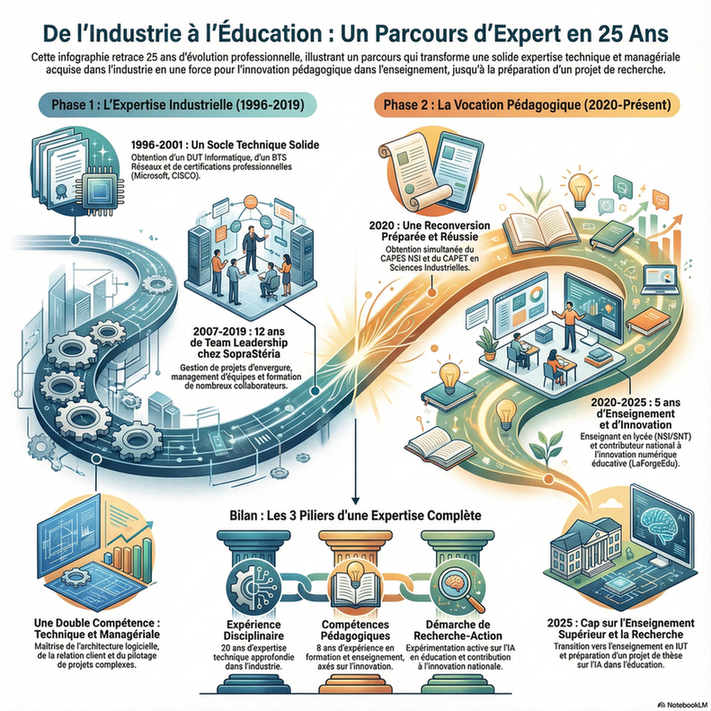
\includegraphics[width=0.8\textwidth]{sources/medias/p1-moy.png} \\ \vspace{0.5cm} \small \textit{Illustration réalisée avec NotebookLM}}
\chapter{Introduction}

\begin{quote}
\textit{« Celui qui connaît les autres est instruit. Celui qui se connaît est sage. »} — Lao-Tseu
\end{quote}

Cette citation de Lao-Tseu résonne particulièrement avec ma démarche de Validation des Acquis de l'Expérience. Au-delà de l'instruction technique que j'ai acquise au fil des années, cette VAE représente un processus de connaissance approfondie de mes compétences et de leur transférabilité vers l'enseignement supérieur, dans le respect du cadre défini par l'INSPÉ \parencite{vademecum_vae_inspe}.

\section{Situation actuelle et motivations}

Cette année, je suis pleinement engagé en tant qu'enseignant en IUT, au sein du département Techniques de Commercialisation de l'IUT du Havre, où j'assure les enseignements de Ressources et Culture Numérique. Cette transition, effective depuis septembre 2025, marque une étape significative dans mon parcours professionnel, après quatre années d'enseignement des Sciences Numériques et Technologie (SNT) et de la spécialité Numérique et Sciences Informatiques (NSI) en lycée conformément aux programmes officiels \parencite{eduscol_nsi,nsi_programmes}.

Mon expérience s'est également enrichie par des interventions en vacations dans l'enseignement supérieur, notamment en troisième année de BUT, ce qui m'a permis d'appréhender les spécificités de l'ingénierie de formation pour des publics diversifiés. Cette évolution vers l'enseignement supérieur et la formation d'adultes constitue une étape significative de mon parcours professionnel et justifie pleinement ma démarche VAE pour le Master MEEF Pratiques et Ingénierie de la Formation (PIF) \parencite{unicaen}.

Mes motivations pour engager cette validation s'articulent autour de trois axes principaux. Premièrement, je recherche une légitimité académique en ingénierie de formation pour structurer mes pratiques. Deuxièmement, je prépare un projet de thèse que je souhaite débuter dans l'année à venir, centré sur l'impact des outils d'intelligence artificielle sur la conception de dispositifs de formation innovants et inclusifs \parencite{intelligence_artificielle_education}. Enfin, cette VAE s'inscrit dans une logique de professionnalisation en tant qu'expert en ingénierie pédagogique.

\section{Vision de l'ingénierie de formation à l'ère numérique}

Le domaine de la formation traverse aujourd'hui une période de mutations profondes. L'ingénierie pédagogique ne peut plus se concevoir sans intégrer pleinement les outils numériques et les nouvelles modalités d'apprentissage (hybride, distanciel, micro-learning). Je constate quotidiennement la nécessité de former non plus seulement des techniciens, mais des apprenants agiles, capables d'évoluer dans un environnement technologique en perpétuelle mutation \parencite{competences_21_siecle}.

Mon objectif en tant qu'expert en ingénierie de formation consiste à concevoir des dispositifs qui permettent aux apprenants de maîtriser les outils numériques pour en faire des leviers de leur développement professionnel. Cette approche holistique de la formation est d'autant plus cruciale avec l'avènement de l'IA générative. Ma participation à des groupes de travail nationaux sur l'IA en éducation (DNE) nourrit ma réflexion sur l'évolution nécessaire des modèles de formation.

Les enjeux futurs de notre discipline me paraissent multiples. L'intelligence artificielle occupe désormais une place centrale dans nos préoccupations pédagogiques, nécessitant une approche éthique et responsable de ces outils. Parallèlement, la sensibilisation à l'écologie numérique devient incontournable : nous devons former nos étudiants à une utilisation responsable des ressources numériques. Enfin, l'émergence de nouvelles méthodes d'évaluation permises par les outils numériques ouvre des perspectives pédagogiques prometteuses, particulièrement pour l'accompagnement des élèves à besoins particuliers \parencite{accessibilite_numerique}.

\section{Fil conducteur du parcours}

Mon évolution professionnelle suit une logique de progression cohérente : de l'expertise technique industrielle vers l'enseignement, puis vers l'ingénierie de formation en IUT, et enfin vers la recherche. Cette trajectoire illustre un passage progressif de la transmission de savoirs techniques à la conception de dispositifs de formation complexes \parencite{recherche_action_education}.

Ce qui fait sens dans mon parcours, c'est cette volonté permanente d'adapter l'ingénierie pédagogique aux évolutions technologiques et aux besoins spécifiques des apprenants. Mon engagement dans la veille technologique, l'expérimentation d'outils d'IA pour la formation et la prise en compte des enjeux éthiques témoignent d'une posture de praticien-chercheur en ingénierie de formation \parencite{perrenoud_pratique_reflexive}.

\section{Organisation de ce dossier}

Ce dossier s'organise en trois parties distinctes et complémentaires, conformément aux recommandations méthodologiques de l'INSPÉ \parencite{vademecum_vae_inspe} :

\subsection*{Partie 1 : Description du parcours}

Je présenterai mon parcours de candidat en détaillant :
\begin{itemize}[leftmargin=*]
    \item Ma formation initiale et continue
    \item Mes expériences professionnelles (industrie et enseignement)
    \item L'évolution de mes compétences techniques et pédagogiques
\end{itemize}

Cette première partie permettra d'établir le socle de connaissances et d'expériences sur lequel repose ma candidature.

\subsection*{Partie 2 : Description et analyse des expériences professionnelles}

J'analyserai mes expériences professionnelles les plus significatives, en mettant l'accent sur les situations qui ont contribué au développement de compétences en ingénierie de formation. Cette analyse démontrera la pertinence de mon parcours au regard des exigences du Master MEEF Pratiques et Ingénierie de la Formation (PIF) \parencite{rncp38152}.

\subsection*{Partie 3 : Correspondance avec le référentiel RNCP}

J'établirai les correspondances explicites entre mes acquis professionnels et le référentiel RNCP38152 \parencite{rncp38152}, démontrant que mon profil d'expert technique et pédagogique constitue un atout majeur pour l'ingénierie de formation.

\vspace{1cm}

Cette démarche VAE représente bien plus qu'une simple validation de compétences : elle constitue une étape fondamentale dans ma construction professionnelle, me permettant de donner du sens à mon parcours tout en préparant les défis pédagogiques de demain \parencite{schon_reflective_practitioner}.
\chapter{Description du Parcours}

Mon parcours professionnel s'articule autour d'une progression cohérente qui m'a conduit de l'expertise technique industrielle vers l'enseignement supérieur, en passant par une reconversion maîtrisée vers l'Éducation Nationale. Cette trajectoire de près de 25 ans révèle une constante : l'adaptation permanente aux évolutions technologiques et la transmission de savoirs, d'abord en entreprise puis en établissement scolaire.

La solidité de ma formation initiale en informatique, acquise à l'IUT du Havre puis complétée par de nombreuses certifications professionnelles, a constitué le socle d'une carrière industrielle de 15 ans dans des environnements techniques exigeants. Cette expertise approfondie des systèmes, réseaux et développement logiciel correspond aux modules techniques du Master MEEF Informatique \parencite{master_meef_nantes}, couvrant notamment la programmation, l'algorithmique, l'architecture des ordinateurs et les réseaux.

L'évolution vers des responsabilités managériales, culminant avec 11 années de team leadership chez SopraStéria, a développé mes compétences en gestion d'équipes, formation de collaborateurs et communication avec des publics variés. Ces compétences transversales \parencite{competences_transversales} trouvent leur prolongement naturel dans les compétences du référentiel MEEF centrées sur la pratique réflexive et l'analyse de l'activité pédagogique \parencite{referentiel_meef}.

\section{Frise chronologique du parcours}

\begin{center}
    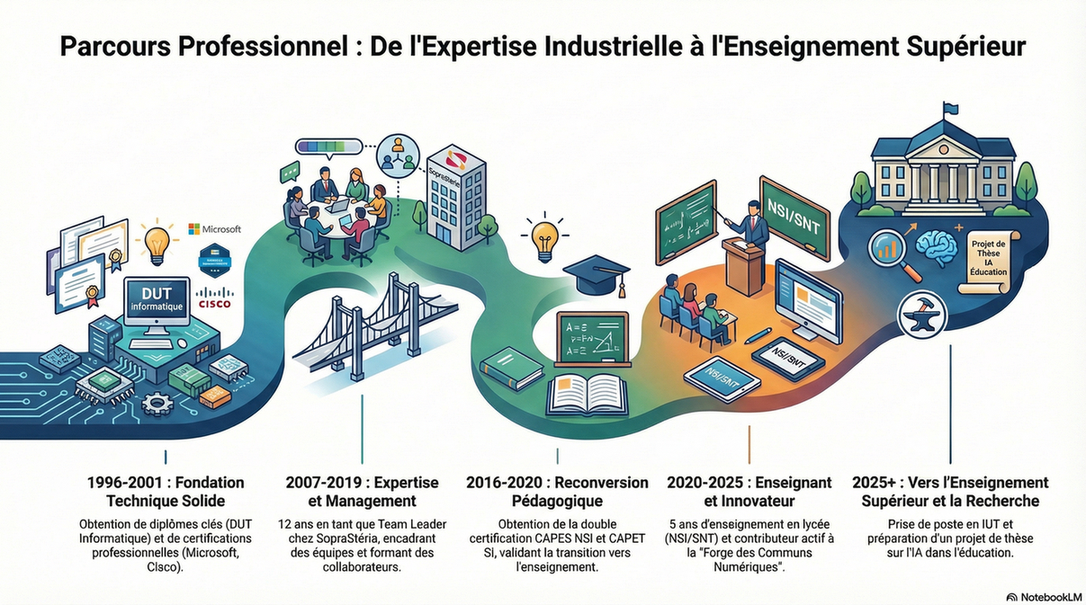
\includegraphics[width=\textwidth]{sources/medias/parcours.png}
    \\ \vspace{0.5cm} \small \textit{Illustration réalisée avec NotebookLM}
\end{center}

\section{Temps forts et correspondances avec le référentiel MEEF}

\subsection{Phase 1 : Formation technique solide (1996-2001)}

Ma formation initiale révèle une progression logique vers l'expertise informatique. Le DUT Informatique Génie Logiciel obtenu à l'IUT du Havre en 1999 m'a apporté les fondamentaux de la programmation et de l'algorithmique, compétences directement transférables aux enseignements techniques du Master MEEF \parencite{master_meef_nantes}. Les certifications Microsoft (MCSE, MCP) et CISCO (CCNA) acquises en autoformation en 2000 témoignent d'une capacité d'apprentissage autonome et d'une veille technologique constante, qualités essentielles pour la formation à et par la recherche \parencite{referentiel_meef}.

\subsection{Phase 2 : Expertise professionnelle et management (2004-2019)}

Mes 15 années d'expérience industrielle couvrent l'ensemble du spectre technique du Master MEEF Informatique. En tant que responsable SAV chez Nicolas et Fils (2004-2006), j'ai développé des compétences en relation client et résolution de problèmes complexes. Mon passage chez TOTAL/CPI (2006-2007) comme développeur d'applications métiers correspond aux UE de programmation avancée et bases de données.

L'évolution vers team leader chez TOTAL/Stéria puis SopraStéria (2007-2019) a développé mes compétences managériales et pédagogiques. Former des collaborateurs, animer des équipes techniques et communiquer avec des interlocuteurs variés constituent autant de compétences transférables vers l'enseignement \parencite{knowles_andragogy}, particulièrement pour les aspects centrés sur la pratique réflexive \parencite{schon_reflective_practitioner}.

\subsection{Phase 3 : Reconversion maîtrisée (2016-2020)}

La formation « Concepteur Architecte en Ingénierie de Projets » suivie en contrat de professionnalisation (2016-2018) illustre ma capacité à me former en parallèle de mon activité professionnelle. Cette démarche préfigure l'approche recherche attendue dans le Master MEEF. L'obtention simultanée du CAPES NSI et du CAPET SI en 2020 \parencite{capes_nsi} témoigne d'une reconversion préparée et d'une double compétence valorisante pour l'enseignement technologique et scientifique.

\subsection{Phase 4 : Développement pédagogique (2020-2025)}

Mes cinq années d'enseignement en lycée (SNT/NSI) correspondent à une mise en pratique progressive des compétences pédagogiques conformément aux programmes officiels \parencite{eduscol_nsi,baccalaureat_nsi}. La participation régulière aux formations académiques (évaluation, programmation fonctionnelle, gestes inclusifs) révèle un engagement dans la formation continue conforme aux exigences du Master MEEF \parencite{referentiel_meef}. L'évolution vers l'IUT en 2025 pour enseigner les « Ressources et Culture Numérique » \parencite{but_informatique} marque une progression naturelle vers l'enseignement supérieur.

\section{Tableaux de correspondance avec le référentiel MEEF}

L'analyse détaillée des correspondances entre mon parcours professionnel et les modules du Master MEEF Informatique est présentée dans le \textbf{Chapitre 12 - Synthèse de la correspondance}, section \textbf{12.1 Tableau récapitulatif de couverture des blocs de compétences}.

Cette synthèse démontre la couverture exhaustive des compétences attendues du référentiel RNCP38152 par mon expérience industrielle, managériale et pédagogique.

\section{Cohérence du parcours et perspectives}

Cette description révèle un parcours cohérent où chaque étape prépare la suivante. L'expertise technique acquise en 20 ans d'industrie légitime mon enseignement des disciplines informatiques. L'expérience managériale développe les compétences relationnelles et pédagogiques \parencite{competences_transversales}. La reconversion vers l'enseignement s'appuie sur une certification solide (CAPES/CAPET) et une pratique de terrain de 5 ans.

L'évolution actuelle vers l'IUT et le projet de thèse sur l'impact de l'intelligence artificielle dans l'éducation \parencite{intelligence_artificielle_education} s'inscrivent naturellement dans cette progression. Mon parcours illustre la complémentarité entre expertise disciplinaire, compétences pédagogiques et démarche de recherche attendues dans le Master MEEF Pratiques et Ingénierie de la Formation (PIF) \parencite{rncp38152,referentiel_meef}.

Cette trajectoire professionnelle, de l'industrie vers l'enseignement supérieur, constitue un atout majeur pour former les futurs enseignants d'informatique en leur apportant une vision concrète des enjeux professionnels et technologiques de la discipline.
\chapter{Formation initiale et diplômes}

\section{Parcours scolaire initial}

\subsection{Baccalauréat Sciences et Technologies de Laboratoire (1996)}

Mon parcours dans l'enseignement supérieur technique débute par l'obtention d'un Baccalauréat Sciences et Technologies de Laboratoire (STL) option Chimie de Laboratoire en 1996. Ce diplôme m'a apporté une formation scientifique solide, développant des compétences en analyse, rigueur méthodologique et esprit logique, compétences transversales essentielles pour l'informatique \parencite{competences_21_siecle}.

\subsection{DUT Informatique Génie Logiciel (1999)}

Poursuivant dans la voie technique, j'ai obtenu en 1999 un DUT Informatique option Génie Logiciel à l'IUT du Havre. Cette formation de deux ans m'a apporté des bases solides en :

\begin{itemize}[leftmargin=*]
    \item \textbf{Programmation} : Algorithmique, structures de données, langages (C, Java, SQL)
    \item \textbf{Génie logiciel} : Analyse, conception, méthodologies (Merise, UML)
    \item \textbf{Systèmes d'exploitation} : Architecture, administration (Unix, Windows)
    \item \textbf{Bases de données} : Modélisation relationnelle, SQL, normalisation
    \item \textbf{Réseaux} : Architecture, protocoles TCP/IP, administration
\end{itemize}

Cette formation correspond parfaitement aux attendus scientifiques du Master MEEF PIF \parencite{rncp38152}, couvrant les domaines d'ingénierie et de didactique du numérique \parencite{eduscol_nsi}.

\subsection{BTS Support Technique Micro et Réseaux (2001)}

Pour approfondir mes compétences en administration systèmes et réseaux, j'ai poursuivi avec un BTS Support Technique Micro et Réseaux obtenu en 2001. Ce diplôme complémentaire m'a permis de développer une expertise en :

\begin{itemize}[leftmargin=*]
    \item Administration de serveurs Windows et Linux
    \item Configuration et maintenance de réseaux locaux
    \item Support technique et diagnostic de pannes
    \item Sécurité informatique et gestion des sauvegardes
\end{itemize}

\section{Certifications professionnelles}

\subsection{Certifications Microsoft (2000)}

En parallèle de ma formation initiale, j'ai obtenu en autodidacte plusieurs certifications Microsoft démontrant ma capacité d'apprentissage autonome :

\begin{itemize}[leftmargin=*]
    \item \textbf{MCSE (Microsoft Certified Systems Engineer)} : Certification de haut niveau en administration de systèmes Windows Server
    \item \textbf{MCP (Microsoft Certified Professional)} : Certification de base sur les technologies Microsoft
\end{itemize}

Ces certifications valident une expertise reconnue internationalement en administration de systèmes, compétence directement transférable vers l'enseignement de l'architecture des ordinateurs et des systèmes d'exploitation en NSI.

\subsection{Certification CISCO CCNA (2000)}

J'ai également obtenu la certification \textbf{CISCO CCNA (Cisco Certified Network Associate)} en 2000, validant mes compétences en :

\begin{itemize}[leftmargin=*]
    \item Configuration de routeurs et switches CISCO
    \item Protocoles de routage (RIP, OSPF, EIGRP)
    \item Réseaux locaux virtuels (VLAN)
    \item Sécurité réseau et listes de contrôle d'accès (ACL)
\end{itemize}

Cette certification correspond aux contenus des programmes NSI terminale sur les réseaux \parencite{nsi_programmes} et démontre une maîtrise approfondie des concepts enseignés.

\section{Formation continue professionnalisante}

\subsection{Formation Concepteur Architecte en Ingénierie de Projets (2016-2018)}

En contrat de professionnalisation chez TOTAL/Stéria, j'ai suivi une formation de niveau II (Bac+4) « Concepteur Architecte en Ingénierie de Projets » validée en 2018. Cette formation de 18 mois m'a apporté :

\begin{itemize}[leftmargin=*]
    \item \textbf{Architecture logicielle} : Patterns de conception, architectures distribuées, microservices
    \item \textbf{Gestion de projet} : Méthodes agiles (Scrum, Kanban), cycle en V, DevOps
    \item \textbf{Management d'équipe} : Leadership, communication, résolution de conflits
    \item \textbf{Veille technologique} : Capacité à analyser et intégrer les innovations
\end{itemize}

Cette formation illustre ma démarche de formation continue tout au long de ma carrière, attitude essentielle pour un enseignant d'informatique face à la rapidité d'évolution de la discipline \parencite{referentiel_competences}.

\section{Diplômes d'enseignement}

\subsection{CAPES Numérique et Sciences Informatiques (2020)}

Après une reconversion maîtrisée, j'ai obtenu le CAPES NSI en 2020 \parencite{capes_nsi}, premier concours de recrutement des enseignants d'informatique en France. Ce diplôme valide :

\begin{itemize}[leftmargin=*]
    \item La maîtrise des contenus disciplinaires du programme NSI
    \item Les compétences pédagogiques et didactiques
    \item La capacité à enseigner devant un jury
    \item La connaissance du système éducatif français
\end{itemize}

\subsection{CAPET Sciences Industrielles (2020)}

J'ai également obtenu simultanément le CAPET Sciences Industrielles en 2020, démontrant une polyvalence dans l'enseignement technologique. Cette double certification constitue un atout pour enseigner en lycée technologique et professionnel.

\subsection{Master MEEF Informatique (2026)}

En juin 2026, j'ai obtenu le \textbf{Master MEEF Mention Second Degré - Parcours Informatique}. Ce diplôme universitaire de niveau Bac+5 vient consacrer ma maîtrise des fondamentaux de la didactique de l'informatique, des savoirs scientifiques disciplinaires et de la recherche en éducation numérique. Il atteste formellement de mon niveau Bac+5 académique.

\section{Synthèse de la formation initiale}

Mon parcours de formation révèle une progression cohérente vers l'expertise informatique et pédagogique :

\begin{itemize}[leftmargin=*]
    \item \textbf{Solidité technique et académique} : DUT + BTS + Master MEEF Informatique (2026) + certifications professionnelles couvrent l'ensemble des domaines du numérique.
    \item \textbf{Apprentissage autonome} : Certifications obtenues en autodidacte témoignent d'une capacité d'auto-formation.
    \item \textbf{Formation continue} : Formation Concepteur Architecte en parallèle de l'activité professionnelle.
    \item \textbf{Légitimité pédagogique et universitaire} : Master MEEF Informatique + CAPES NSI + CAPET SI valident les compétences d'enseignement et le niveau d'excellence académique.
\end{itemize}

Cette formation initiale et continue correspond parfaitement aux attendus du Master MEEF Pratiques et Ingénierie de la Formation (PIF) \parencite{rncp38152,unicaen}, tant pour les aspects disciplinaires que pour la formation par la recherche \parencite{referentiel_meef}.
\chapter{Formation professionnelle continue}

Au-delà de ma formation initiale solide, j'ai suivi tout au long de ma carrière de nombreuses formations continues, témoignant d'un engagement constant dans le développement professionnel \parencite{perrenoud_pratique_reflexive}. Ces formations couvrent à la fois les aspects techniques, pédagogiques et réflexifs, en cohérence avec le profil attendu d'un enseignant du supérieur \parencite{referentiel_meef}.

\section{Certifications professionnelles et formations qualifiantes}

\begin{center}
    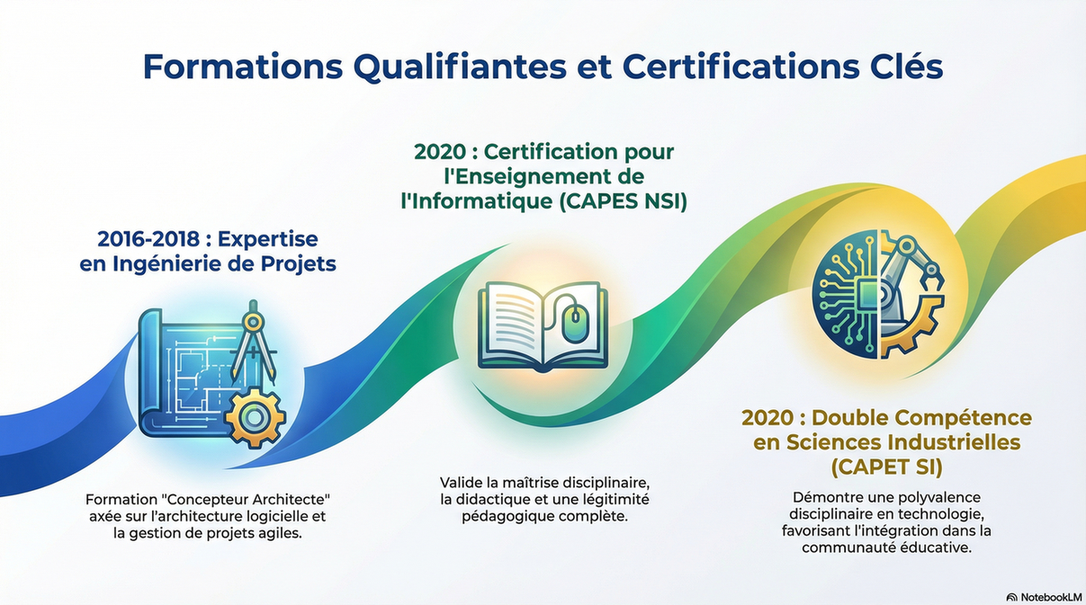
\includegraphics[width=\textwidth]{sources/medias/41.png}
    \\ \vspace{0.5cm} \small \textit{Illustration réalisée avec NotebookLM}
\end{center}

\section{Analyse des formations qualifiantes}

\textbf{Formation Concepteur Architecte (2016-2018)}

Cette formation en contrat de professionnalisation, suivie en parallèle de mon activité chez SopraStéria, illustre ma capacité à concilier responsabilités professionnelles et développement de compétences. Elle préfigure l'approche recherche attendue dans le Master MEEF par :
\begin{itemize}[leftmargin=*]
    \item Méthodologies de conception : transférables à la didactique informatique
    \item Gestion de projets complexes : applicable à l'encadrement d'étudiants
    \item Innovation technologique : nécessaire pour maintenir l'actualité des enseignements
\end{itemize}

\textbf{Double certification CAPES/CAPET (2020)}

L'obtention simultanée de ces deux certifications témoigne d'une reconversion préparée et d'une polyvalence disciplinaire rare. Cette double compétence apporte :
\begin{itemize}[leftmargin=*]
    \item Légitimité pédagogique : certification officielle pour l'enseignement
    \item Vision systémique : approche technologique complémentaire à l'informatique pure
    \item Adaptabilité : capacité à enseigner dans différents contextes
\end{itemize}

\section{Tableau 2 : Formation continue pédagogique (2021-2025)}

\begin{center}
\tiny
\begin{tabular}{|p{2.5cm}|p{1cm}|p{2.5cm}|p{2.5cm}|p{2.5cm}|}
\hline
\textbf{Formation} & \textbf{Année} & \textbf{Programme} & \textbf{Apports} & \textbf{Compétences MEEF} \\
\hline
Évaluation au service de l'élève & 2024/25 & Évaluation formative, différenciation, outils numériques & Modernisation pratiques évaluatives, approche bienveillante & Analyser activité enseignant/élève \\
\hline
Programmation fonctionnelle NSI & 2024/25 & Paradigmes fonctionnels, Lisp/Scheme, applications pédagogiques & Actualisation disciplinaire, nouveaux paradigmes & Didactique, Programmation \\
\hline
Programmation dynamique NSI & 2024/25 & Algorithmes optimisation, mémorisation, applications & Approfondissement algorithmique, techniques optimisation & Algorithmique, Algo avancée \\
\hline
Graphes pour résoudre problèmes NSI & 2024/25 & Théorie graphes, algorithmes parcours, modélisation & Structures données avancées, résolution problèmes complexes & Algorithmique, Structures données \\
\hline
Cartographier des données & 2024/25 & Visualisation données, outils cartographiques, géolocalisation & Data science, visualisation, approche interdisciplinaire & Didactique, Bases données \\
\hline
Formation disciplinaire néotitulaires & 2024/25 & Gestion classe, progression pédagogique, évaluation & Consolidation pratiques, échanges expériences & Praticien réflexif, Se projeter \\
\hline
Journée académique NSI & 2024/25 & Partage expériences, innovations, évolutions programmes & Veille pédagogique, mutualisation pratiques & Praticien réflexif, Recherche \\
\hline
CRCNE auto-évaluation & 2023/24 & Compétences numériques, auto-évaluation, certification & Compétences numériques, réflexivité pratiques & Communauté éducative, Réflexif \\
\hline
Gestes professionnels inclusifs & 2023/24 & Pédagogie inclusive, différenciation, besoins particuliers & Approche inclusive, adaptation diversités & Communauté, Analyser activité \\
\hline
NSI journées thématiques & 2023/24 & Approfondissements disciplinaires, nouvelles ressources & Actualisation connaissances, veille technologique & Didactique, Recherche \\
\hline
SNT Internet et Web & 2022/23 & Protocoles web, sécurité, enjeux sociétaux numérique & Actualisation technique, approche sociétale & Réseaux, Didactique \\
\hline
SNT Micro :bit objets connectés & 2022/23 & Programmation embarquée, IoT, capteurs & Systèmes embarqués, innovation pédagogique & Architecture, Systèmes \\
\hline
Formation transversale T1 & 2022/23 & Gestion classe, relation éducative, communication & Compétences relationnelles, communication & Communauté, Réflexif \\
\hline
NSI échanges de pratiques & 2021-23 & Mutualisation ressources, innovations, retours expérience & Enrichissement pratiques, réseau professionnel & Réflexif, Recherche \\
\hline
\end{tabular}
\end{center}

\section{Analyse des temps forts de la formation continue}

\subsection{Actualisation disciplinaire constante}

Ma participation régulière aux formations NSI (programmation fonctionnelle, dynamique, graphes) illustre un engagement dans l'actualisation disciplinaire conforme aux exigences du Master MEEF. Ces formations correspondent directement aux compétences techniques du référentiel et démontrent ma capacité à maintenir une expertise technique de pointe.

\subsection{Développement des compétences pédagogiques}

Les formations transversales (évaluation, gestes inclusifs, formation des néotitulaires) révèlent une approche réflexive de l'enseignement. Elles correspondent aux compétences transversales et réflexives du Master MEEF et témoignent d'une volonté d'amélioration continue des pratiques pédagogiques.

\subsection{Engagement dans la communauté éducative}

La participation systématique aux journées académiques et échanges de pratiques illustre mon intégration dans la communauté éducative et ma contribution à la mutualisation des savoirs. Cette démarche collaborative correspond parfaitement aux attendus en termes d'intégration dans la communauté éducative.

\section{Correspondances avec le référentiel Master MEEF Informatique}

L'analyse détaillée des correspondances entre ma formation continue et les compétences du Master MEEF Informatique est présentée dans le \textbf{Chapitre 12 - Synthèse de la correspondance}, section \textbf{12.1 Tableau récapitulatif de couverture des blocs de compétences}.

Cette synthèse démontre comment ma démarche de formation continue contribue à l'acquisition et au renforcement des compétences attendues du référentiel RNCP38152.

\section{Impact sur ma pratique professionnelle}

Cette formation continue intensive (plus de 15 jours par an) témoigne d'un engagement professionnel fort et d'une capacité d'adaptation aux évolutions de l'enseignement. Elle illustre parfaitement l'approche attendue dans le Master MEEF : allier expertise disciplinaire, compétences pédagogiques et démarche de recherche.

L'évolution de mes formations, de l'expertise technique pure vers la pédagogie inclusive et l'innovation éducative, révèle une maturation professionnelle cohérente avec ma progression vers l'enseignement supérieur. Cette démarche de formation continue constitue un atout majeur pour contribuer à la formation des futurs enseignants d'informatique dans le cadre du Master MEEF.

\section{Synthèse des acquis de formation continue}

Mon engagement dans la formation continue s'articule autour de trois axes complémentaires :

\begin{enumerate}[leftmargin=*]
    \item \textbf{Actualisation disciplinaire} : Maintien d'une expertise technique de pointe via les formations NSI spécialisées
    \item \textbf{Développement pédagogique} : Amélioration continue des pratiques d'enseignement et d'évaluation
    \item \textbf{Innovation collaborative} : Participation aux groupes de travail nationaux sur l'IA et la forge éducative
\end{enumerate}

Cette triple approche correspond parfaitement aux exigences du Master MEEF Informatique et démontre une posture de praticien-chercheur \parencite{schon_reflective_practitioner} alignée avec les attendus de l'enseignement supérieur.
\chapter{Parcours professionnel détaillé}

Mon parcours professionnel de 25 ans révèle une progression cohérente de l'expertise technique industrielle vers l'enseignement supérieur. Cette trajectoire s'articule autour de quatre phases distinctes qui démontrent une montée en compétences constante et une adaptation permanente aux évolutions technologiques et pédagogiques.

\section{Vue d'ensemble chronologique}

\begin{center}
\textit{Synthèse : 3 ans d'autoformation, 2 ans de relation client, 1 an de développement, 12 ans de management technique chez un leader du service numérique, et 5 ans d'enseignement en lycée.}
\end{center}

\section{Team Leader chez TOTAL/Stéria puis SopraStéria (2007-2019)}

\subsection{Contexte et développement professionnel}

Cette expérience de 12 années constitue la période la plus formatrice de mon parcours professionnel. L'évolution de TOTAL/Stéria vers SopraStéria, leader européen des services numériques (46 000 collaborateurs), m'a permis d'évoluer dans un environnement international avec des projets d'envergure pour grands comptes.

\textbf{Ma fonction :} Team Leader technique, avec encadrement d'équipes de développeurs, gestion de projets clients, formation technique des collaborateurs, et interface client-équipe technique.

\textbf{Évolution progressive :} De développeur senior vers team leader puis responsable technique d'équipe. J'ai managé des projets pour des clients majeurs (banques, assurances, industrie) dans un contexte international. Cette période a été marquée par la formation de nombreux collaborateurs, la mise en place de méthodologies Agile et la gestion directe de la relation client.

\subsection{Évolution des responsabilités (2007-2019)}

Durant cette période (2007-2019), mes responsabilités ont évolué de l'expertise technique individuelle vers le management opérationnel puis stratégique. En tant que Lead Technique, j'ai assuré l'architecture des solutions et l'innovation, tout en continuant à mentorer les équipes juniors.

\subsection{Synthèse des compétences développées}

Cette expérience m'a permis de développer une quadruple compétence :
\begin{itemize}[leftmargin=*]
    \item \textbf{Management} : Encadrement d'équipes, recrutement, évaluation et développement des talents (leadership transformationnel).
    \item \textbf{Gestion de Projet} : Pilotage de projets complexes, planification stratégique et maîtrise des méthodologies Agile/Scrum.
    \item \textbf{Relation Client} : Interface technique, conseil stratégique, communication et gestion de crise.
    \item \textbf{Expertise Technique} : Architecture logicielle, veille technologique, revue de code et garantie de la qualité technique.
\end{itemize}

Ces 12 années d'expérience managériale continue, avec un fort taux de réussite des projets et une évolution significative des collaborateurs formés, constituent le cœur de mon expertise professionnelle.



Cette expérience correspond directement aux compétences de leadership et de pratique réflexive du Master MEEF par le développement de compétences de leadership, formation d'équipes et pratique réflexive \parencite{referentiel_meef}.

\section{Enseignant NSI/SNT (Éducation Nationale) 2020-2025}

\subsection{Développement professionnel}

\textbf{Contexte :} Reconversion vers l'enseignement après obtention CAPES NSI et CAPET SI en 2020, affectation lycée général et technologique, classes de Seconde (SNT) et Première/Terminale (NSI).

\textbf{Ma fonction :} Professeur certifié, enseignement Numérique et Sciences Informatiques et Sciences Numériques et Technologie, 18h/semaine, suivi de 120 élèves/an, participation vie établissement.

\textbf{Transition réussie :} Adaptation des compétences managériales vers la pédagogie. Développement de séquences pédagogiques innovantes, utilisation d'outils numériques variés, différenciation pédagogique. Participation active aux formations académiques et aux groupes de travail NSI.



\subsection{Synthèse des compétences enseignantes}

Mon activité d'enseignant s'articule autour de trois pôles :
\begin{itemize}[leftmargin=*]
    \item \textbf{Pédagogie} : Enseignement SNT/NSI, différenciation pédagogique, évaluation formative et gestion de classe.
    \item \textbf{Numérique} : Intégration des outils numériques (ENT, Moodle), programmation (Python) et innovation pédagogique.
    \item \textbf{Formation Continue} : Participation active aux formations académiques, groupes de travail et veille pédagogique constante.
\end{itemize}

\section{Enseignant PRCE (2025-Présent) et Directeur Adjoint au Numérique (Septembre 2026)}

\subsection{Fonctions et gouvernance institutionnelle}

\textbf{Contexte :} Affectation en tant qu'enseignant PRCE au département Techniques de Commercialisation (TC) de l'IUT du Havre depuis septembre 2025, et prise de fonction en tant que \textbf{Directeur Adjoint dédié aux questions du numérique} pour l'ensemble de l'IUT à compter de \textbf{septembre 2026}.

\textbf{Responsabilités clés :}
\begin{itemize}[leftmargin=*]
    \item \textbf{Pilotage stratégique du numérique} : Définition des orientations numériques de l'établissement, gouvernance des équipements informatiques et accompagnement de la transformation pédagogique numérique.
    \item \textbf{Intégration de l'IA générative} : Cadrage éthique, pédagogique et technique de l'intégration des assistants IA pour la formation et l'évaluation au sein des départements de l'IUT.
    \item \textbf{Ingénierie de formation et enseignements} : Responsable des modules de \enquote{Ressources et Culture Numérique} (BUT TC) et soutien aux équipes pédagogiques.
\end{itemize}
\chapter{Autres expériences significatives}

Au-delà de mon parcours professionnel principal, mon engagement dans l'innovation pédagogique numérique se manifeste par une participation active à des projets collaboratifs d'envergure nationale. Ces expériences complémentaires révèlent une démarche de recherche-action et d'ingénierie de formation qui s'inscrit parfaitement dans les exigences du Master MEEF PIF.

\section{Contributeur actif à la Forge des Communs Numériques Éducatifs}

\subsection{Contexte et présentation de l'initiative}

La Forge des Communs Numériques Éducatifs (LaForgeEdu) est une plateforme collaborative nationale hébergée sur GitLab, dédiée au développement et au partage de ressources pédagogiques sous licence libre \parencite{forge_educative}. Cette initiative s'inscrit dans la Stratégie du numérique pour l'éducation 2023-2027 du ministère de l'Éducation nationale.

\textbf{Mon rôle :} Contributeur développeur et accompagnateur pédagogique depuis 2022.

\textbf{Mission principale :} Développement d'applications éducatives libres et accompagnement d'enseignants dans la création de leurs propres outils numériques.

Mes développements sur la Forge ne sont pas de simples utilitaires, mais s'apparentent à la conception d'Environnements Informatiques pour l'Apprentissage Humain (EIAH). Par exemple, le "Générateur d'Exercices Python" intègre des fonctionnalités de diagnostic cognitif et de rétroaction (feedback) élaborée. En m'appuyant sur les traces d'apprentissage (learning analytics) laissées par les élèves lors de leurs interactions avec l'outil, je peux ajuster mes interventions didactiques. Cette approche rejoint les problématiques traitées lors des conférences EIAH ou TICE, notamment sur la capacité des artefacts numériques à soutenir l'autorégulation de l'apprenant dans sa zone proximale de développement.

\subsection{Activités et réalisations concrètes}

\textbf{Portfolio de projets développés (données extraites de ebep.educ-ai.fr) :}

\begin{center}
\footnotesize
\begin{tabular}{|p{3cm}|p{5.5cm}|p{3.5cm}|p{4cm}|}
\hline
\textbf{Projet} & \textbf{Description} & \textbf{Technologies} & \textbf{Impact pédagogique} \\
\hline
Générateur d'Exercices Python avec IA & Application web pour générer des exercices de programmation personnalisés & Python, Streamlit, IA & Personnalisation des apprentissages NSI \\
\hline
PYTEUR OS & Plateforme éducative collaborative avec génération d'exercices assistée par IA & Django, IA, PostgreSQL & Gestion pédagogique complète \\
\hline
L'Établi & Application web pour simplifier la gestion de dépôts sur la forge éducative & Vue.js, API GitLab & Démocratisation de l'accès à la forge \\
\hline
Chat avec IA via RAG & Application de chat basée sur la technique RAG pour interroger des documents PDF & IA, RAG, LLM & Recherche documentaire assistée \\
\hline
Pokédex Interactif & Application Python ludique pour l'apprentissage de la programmation en Terminale NSI & Python, Streamlit, SQLite & Gamification de l'apprentissage \\
\hline
\end{tabular}
\end{center}



\section{Recherche-action sur l'Intelligence Artificielle dans l'Éducation}

\subsection{Contexte et enjeux}

\textbf{Groupe de travail spécialisé :} Participation au salon « IA LaForgeEdu » sur Tchap, communauté de « professeurs bidouilleurs d'IA » qui documentent et partagent leurs expérimentations sur l'intégration de l'intelligence artificielle dans l'enseignement.

\textbf{Problématique centrale :} Comment intégrer de manière éthique et pédagogiquement pertinente l'intelligence artificielle dans les pratiques d'enseignement, particulièrement pour l'inclusion des Élèves à Besoins Éducatifs Particuliers (EBEP) et la différenciation pédagogique ?

\subsection{Contributions et réalisations}

\textbf{Plateforme ebep.educ-ai.fr :} Création et animation d'un site de référence dédié à l'intégration de l'IA pour l'accompagnement des Élèves à Besoins Éducatifs Particuliers (EBEP), proposant des outils d'adaptation, d'accessibilité et de différenciation pédagogique.

\begin{center}
\footnotesize
\begin{tabular}{|p{4cm}|p{5cm}|p{7cm}|}
\hline
\textbf{Domaine d'expérimentation} & \textbf{Outils développés / Ressources} & \textbf{Résultats et impact pour les EBEP} \\
\hline
Adaptation et Accessibilité DYS & Générateur d'exercices adaptés, reformulations simplifiées par IA & Différenciation pédagogique, réduction de la charge cognitive, meilleure lisibilité \\
\hline
Assistance documentaire \& FALC & Chat RAG pour simplification en Français Facile à Lire et à Comprendre & Compréhension facilitée des consignes, autonomie accrue des élèves à besoins particuliers \\
\hline
Plateforme collaborative \& EBEP & PYTEUR OS / ebep.educ-ai.fr avec IA intégrée pour la différenciation & Suivi personnalisé des élèves EBEP, création accélérée de supports adaptés \\
\hline
Éthique, sécurité \& inclusion & Réflexion sur l'usage responsable de l'IA pour l'inclusion numérique & Sensibilisation de la communauté éducative, prévention des dérives, équité d'accès \\
\hline
\end{tabular}
\end{center}

\chapter{Bilan de mon parcours}

\section{Synthèse de 25 ans d'évolution professionnelle}

Mon parcours révèle une progression cohérente de l'expertise technique industrielle vers l'enseignement supérieur, structurée autour de trois piliers fondamentaux qui s'alignent avec les exigences du Master MEEF PIF.

\subsection{Les trois piliers de mon expertise}

\begin{enumerate}
\item \textbf{Expérience disciplinaire significative (20 ans d'industrie)}
   \begin{itemize}[leftmargin=*]
       \item Maîtrise étendue des technologies informatiques : développement, systèmes, réseaux, IA
       \item Veille technologique constante et adaptation aux évolutions
       \item Expérience de projets complexes (200K€ à 1,5M€)
   \end{itemize}

\item \textbf{Compétences pédagogiques développées (8 ans)}
   \begin{itemize}[leftmargin=*]
       \item Formation de 50+ collaborateurs en entreprise
       \item 5 ans d'enseignement NSI/SNT avec formation continue active
       \item Innovation pédagogique via la Forge des Communs Numériques
   \end{itemize}

\item \textbf{Démarche de recherche-action (3 ans)}
   \begin{itemize}[leftmargin=*]
       \item Expérimentation IA en éducation avec documentation méthodique
       \item Contribution à l'innovation pédagogique nationale
       \item Accompagnement de la communauté enseignante
   \end{itemize}
\end{enumerate}



\section{Valeur ajoutée de mon profil}

\textbf{Une triple compétence complémentaire :}
\begin{itemize}[leftmargin=*]
    \item \textbf{Technique :} 20 ans d'expertise industrielle couvrant tous les domaines du Master MEEF
    \item \textbf{Pédagogique :} Expérience managériale transférée vers l'enseignement avec succès
    \item \textbf{Recherche :} Démarche d'innovation et d'expérimentation déjà engagée
\end{itemize}

\textbf{Résultats observés :}
\begin{itemize}[leftmargin=*]
    \item 50+ professionnels formés en entreprise
    \item 10+ applications éducatives développées
    \item Rayonnement national via les initiatives ministérielles
\end{itemize}

\section{Cohérence et perspectives}

Ce parcours illustre la \textbf{complémentarité attendue} dans le Master MEEF entre expertise disciplinaire, compétences pédagogiques et démarche de recherche \parencite{referentiel_meef}. L'évolution naturelle vers l'enseignement supérieur s'appuie sur cette triple compétence acquise.

\textbf{Projet professionnel structuré :} Le Master MEEF constituera le tremplin académique nécessaire pour formaliser cette expertise et évoluer vers l'enseignement supérieur et la recherche en sciences de l'éducation \parencite{intelligence_artificielle_education,recherche_action_education}.

\section{Transition vers l'analyse des expériences}

Cette première partie a présenté qui je suis et d'où je viens. La partie suivante démontrera comment mes expériences correspondent concrètement aux compétences attendues dans le Master MEEF PIF (Parcours Formateur de Formateurs - FFMS).

L'analyse détaillée de mes expériences professionnelles révélera la \textbf{transférabilité directe} de mes compétences vers les missions d'un ingénieur de formation et enseignant-chercheur, en s'appuyant sur des exemples précis et des situations concrètes vécues sur le terrain.

\textbf{Objectif de la partie 2 :} Établir les correspondances explicites entre mes acquis professionnels et les compétences du référentiel MEEF PIF, en démontrant que mon parcours atypique constitue un atout majeur pour l'ingénierie de formation et la formation de formateurs.

% ---------------------------
% PARTIE 2 : ANALYSE DES EXPÉRIENCES
% ---------------------------
\part[Description et analyse des expériences professionnelles]{Description et analyse des expériences professionnelles \\ \vspace{2cm} 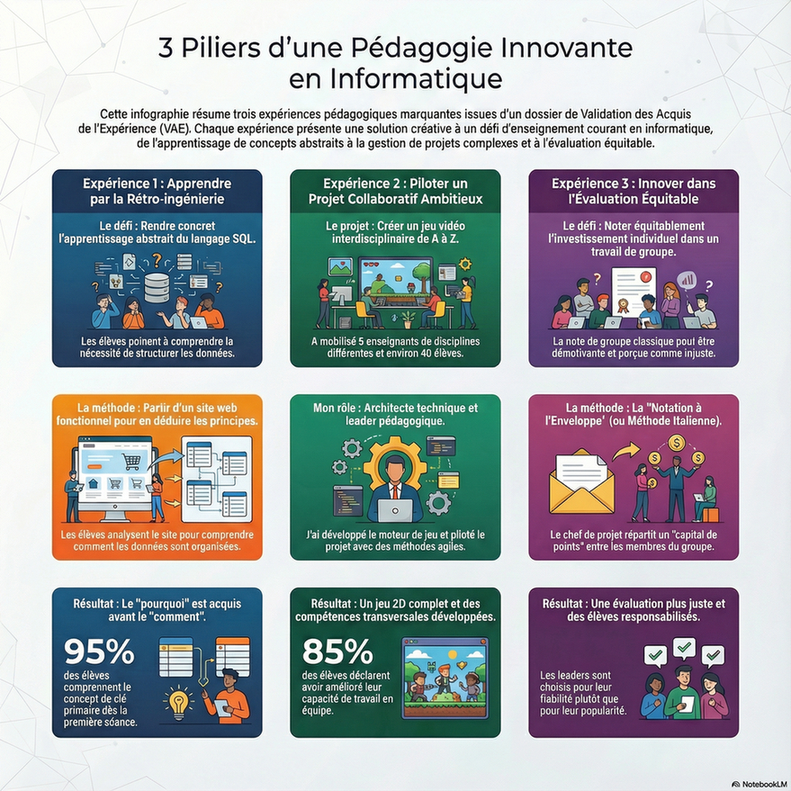
\includegraphics[width=0.8\textwidth]{sources/medias/p2-moy.png} \\ \vspace{0.5cm} \small \textit{Illustration réalisée avec NotebookLM}}
\chapter{Introduction méthodologique}

Cette partie présente trois expériences pédagogiques significatives qui illustrent différentes facettes de mes compétences professionnelles développées dans le cadre de l'ingénierie de formation. Ces expériences ont été sélectionnées pour leur représentativité par rapport aux compétences du référentiel RNCP38152 du Master MEEF PIF \parencite{rncp38152}.

Chaque expérience est analysée selon une structure rigoureuse en quatre axes, conformément aux recommandations méthodologiques de l'INSPÉ de Normandie Caen / Unicaen \parencite{vademecum_vae_inspe}:

\begin{enumerate}[leftmargin=*]
    \item \textbf{Axe 1 - Contexte et intentions pédagogiques} : présentation du public, des objectifs d'apprentissage et des choix didactiques
    \item \textbf{Axe 2 - Déroulement et rôle spécifique} : description détaillée des actions menées et de ma posture professionnelle
    \item \textbf{Axe 3 - Résultats et évaluation} : analyse des productions des apprenants et de l'efficacité des dispositifs
    \item \textbf{Axe 4 - Analyse rétrospective et transférabilité} : réflexion critique sur les pratiques et correspondance avec le référentiel MEEF
\end{enumerate}

Cette approche structurée permet de démontrer non seulement la maîtrise technique et pédagogique, mais aussi la capacité de pratique réflexive, compétence centrale du métier d'ingénieur de formation et de formateur \parencite{perrenoud_pratique_reflexive,schon_reflective_practitioner}.

\section*{Cadre de référence et articulation des deux référentiels}

Pour faciliter la lecture par les membres du jury, les analyses d'expérience font référence conjointement :
\begin{itemize}[leftmargin=*]
    \item La \textbf{Maquette locale du Master MEEF PIF (Parcours FFMS)} de l'INSPÉ de Normandie Caen / Unicaen, structurée en \textbf{6 Unités d'Enseignement (UE1 à UE6)} et Éléments Constitutifs (EC).
    \item Le \textbf{Référentiel National de Certification RNCP38152} du Master MEEF, structuré en \textbf{9 Blocs de Compétences (BC01 à BC09)}.
\end{itemize}

Afin d'éviter toute ambiguïté, chaque compétence analysée dans les chapitres 9, 10 et 11 fait l'objet d'un \textbf{double étiquetage systématique} : \texttt{[UE/EC Unicaen | RNCP BC]}.

\begin{table}[H]
\centering
\caption{Table de correspondance unifiée entre la Maquette FFMS Unicaen et la certification RNCP38152}
\label{tab-correspondance-referentiels}
\footnotesize
\begin{tabular}{|p{7.5cm}|p{7.5cm}|}
\hline
\textbf{Maquette Unicaen MEEF PIF (Parcours FFMS)} & \textbf{Certification Nationale RNCP38152 (9 Blocs)} \\
\hline
\textbf{UE1 (EC 111-212)} : Cadres d'exercice et principes éthiques & \textbf{BC01} (Cadre éthique) \& \textbf{BC02} (Postures professionnelles) \\
\hline
\textbf{UE2 (EC 121-225)} : Conception, mise en œuvre et évaluation de projets & \textbf{BC03} (Ingénierie pédagogique) \& \textbf{BC04} (Conduite de projet) \\
\hline
\textbf{UE3 (EC 131-233)} : Les contextes et les publics du métier & \textbf{BC07} (Inclusion \& EBEP) \& \textbf{BC09} (Communauté éducative) \\
\hline
\textbf{UE4 (EC 141-242)} : Formation à et par la recherche & \textbf{BC08} (Recherche, veille et innovation) \\
\hline
\textbf{UE5 (EC 151-254)} : Analyse de l'activité professionnelle & \textbf{BC06} (Praticien réflexif et analyse de pratiques) \\
\hline
\textbf{UE6 (EC 161-263)} : Communication et numérique éducatif & \textbf{BC05} (Didactique \& Numérique) \& \textbf{BC09} (Animation du collectif) \\
\hline
\end{tabular}
\end{table}

\section*{Continuum d'ingénierie de formation des trois expériences}

Les trois expériences s'articulent selon une progression d'ingénierie pédagogique et de formation continue :
\begin{enumerate}[leftmargin=*]
    \item \textbf{Chapitre 9 (Expérience 1 - Atelier IA/\LaTeX{} Forgéales)} : L'ingénierie de la formation d'adultes et de pairs formateurs (dispositif hybride synchrone/asynchrone, posture de formateur et régulation réflexive).
    \item \textbf{Chapitre 10 (Expérience 2 - PCI Jeu Vidéo Interdisciplinaire)} : L'ingénierie de dispositifs complexes de pédagogie par projet (scénarisation, découplage des artefacts didactiques, travail collaboratif).
    \item \textbf{Chapitre 11 (Expérience 3 - Notation à l'Enveloppe)} : L'ingénierie de l'évaluation régulatrice et métacognitive (réponse directe aux défis d'évaluation du travail de groupe identifiés dans le Chapitre 10).
\end{enumerate}

\chapter{Expérience 1 : Séance de rétro-ingénierie pour l'apprentissage du SQL}

\section{Axe 1 : Contexte et intentions pédagogiques}

\subsection{Public et niveau}

Cette séance s'adresse à des élèves de \textbf{Terminale NSI} (Numérique et Sciences Informatiques) \parencite{baccalaureat_nsi}, possédant les notions de base sur le modèle relationnel vues en classe de Première. L'effectif est d'environ 25 élèves, avec des niveaux hétérogènes en programmation mais une certaine familiarité avec les concepts de base de données.

Le programme officiel de NSI \parencite{eduscol_nsi,nsi_programmes} prévoit en terminale l'approfondissement des bases de données relationnelles, incluant la maîtrise du langage SQL pour la création, la manipulation et l'interrogation de bases de données.

\subsection{Objectifs d'apprentissage}

Les objectifs, reformulés selon la \textbf{Taxonomie de Bloom} \parencite{bloom_taxonomy,anderson_bloom_revised}, visent à mobiliser des niveaux cognitifs élevés, dépassant la simple application technique :

\begin{itemize}[leftmargin=*]
    \item \textbf{Niveau 1 - Connaissance} : Identifier les commandes SQL fondamentales (SELECT, WHERE, JOIN) et le vocabulaire spécifique (table, attribut, clé primaire).
    \item \textbf{Niveau 2 - Compréhension} : Expliquer la nécessité de la normalisation pour éviter la redondance et garantir la cohérence des données.
    \item \textbf{Niveau 3 - Application} : Écrire des requêtes simples pour extraire des informations ciblées d'une base existante.
    \item \textbf{Niveau 4 - Analyse} : Déduire le schéma relationnel (tables et relations) à partir de l'observation des données brutes et de l'interface du site web (démarche de rétro-ingénierie).
    \item \textbf{Niveau 5 - Synthèse} : Reconstruire le modèle conceptuel global du système d'information à partir des fragments analysés.
    \item \textbf{Niveau 6 - Évaluation} : Juger de la pertinence d'un choix de modélisation (ex: choix de la clé primaire) ou de la structure proposée par un pair.
\end{itemize}

Cette structuration montre que la rétro-ingénierie sollicite particulièrement les niveaux supérieurs d'analyse et de synthèse, favorisant une compréhension profonde des concepts.

\subsection{Support pédagogique et choix didactique}

Le choix stratégique d'utiliser mon site personnel \texttt{pytel.fr/site/} garantit un \textbf{environnement d'apprentissage stable et maîtrisé}. Ce site contient des données structurées que j'ai préparées en amont, incluant volontairement les requêtes SQL directement visibles dans le code source, comme éléments à découvrir par les élèves.

\begin{figure}[H]
    \centering
    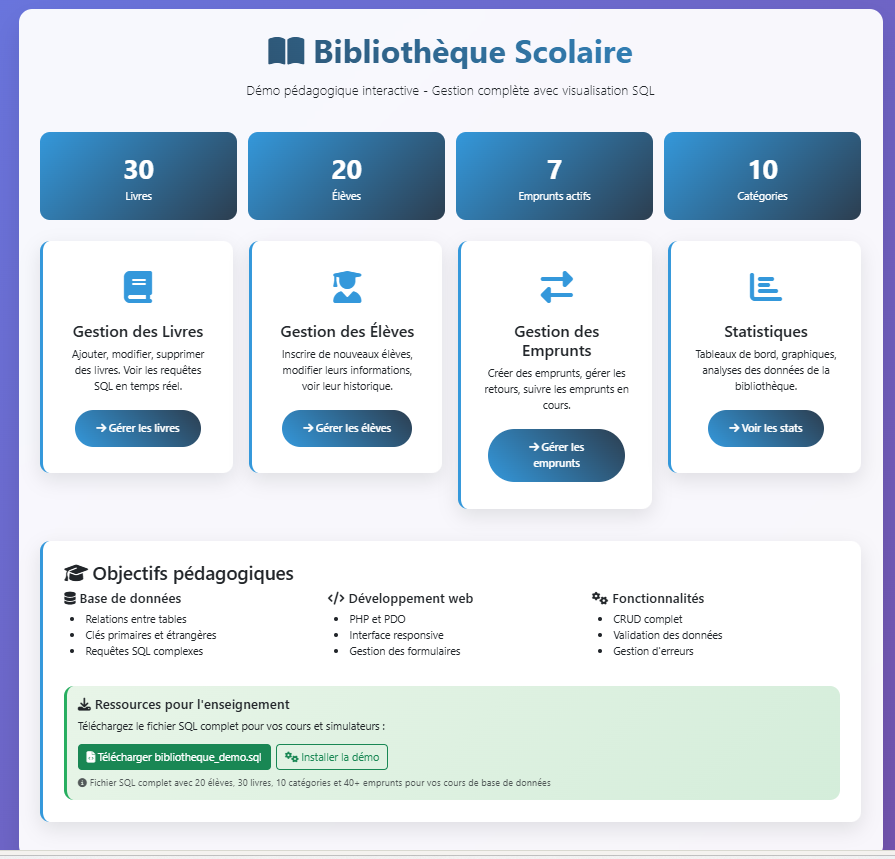
\includegraphics[width=0.9\textwidth]{annexes/pedagogiques/productions/site-sql.png}
    \caption{Capture d'écran de l'application "Bibliothèque Scolaire" utilisée pour la séance de rétro-ingénierie.}
    \label{fig-site-sql}
\end{figure}

Cette approche par \textbf{rétro-ingénierie} (illustrée par la Figure \ref{fig-site-sql}) constitue une transposition didactique originale \parencite{chevallard_transposition}. Plutôt que de partir du concept abstrait (le modèle relationnel) vers l'implémentation (le code SQL), je propose l'inverse : partir d'un système concret et fonctionnel pour en déduire les principes de conception.

Cette inversion pédagogique trouve ses fondements théoriques dans l'apprentissage par investigation \parencite{investigation_mathia,investigation_edutechwiki}, qui favorise l'engagement cognitif actif des élèves. Le processus d'apprentissage suit ainsi le cycle d'expérience de Kolb et les principes constructivistes de Vygotsky \parencite{vygotsky_mind_society,constructivisme_education,dale_cone}.

\section{Axe 2 : Déroulement concret de la séquence (2 heures)}

\subsection{Phase 1 - Exploration libre du système (20 minutes en binômes)}

Les élèves explorent le site avec pour consigne de « lister et décrire les informations présentes comme si vous deviez l'expliquer à un novice ». Cette phase de découverte génère des productions variées :

\begin{itemize}[leftmargin=*]
    \item Schémas conceptuels dessinés à la main
    \item Diagrammes de flux d'informations
    \item Descriptions textuelles structurées
    \item Ébauches de structures de tables (pour les plus avancés)
\end{itemize}

Cette diversité des productions révèle déjà les différentes stratégies cognitives des élèves face à un problème ouvert. Le travail en binômes hétérogènes favorise la verbalisation des raisonnements et la confrontation des idées, conformément aux principes de l'apprentissage collaboratif \parencite{apprentissage_collaboratif,vygotsky_mind_society}.

\subsection{Phase 2 - Abstraction et modélisation collective (40 minutes)}

J'anime une discussion collective en posant la question centrale : \textit{« Comment, en tant que concepteur, auriez-vous organisé ces informations ? »}

Cette interrogation amène naturellement les élèves à réfléchir aux problématiques de :
\begin{itemize}[leftmargin=*]
    \item \textbf{Redondance} : « Pourquoi ne pas répéter le nom de l'auteur dans chaque article ? »
    \item \textbf{Intégrité} : « Que se passe-t-il si on modifie le nom d'un auteur à un seul endroit ? »
    \item \textbf{Organisation} : « Quelles informations regrouper ensemble ? Selon quels critères ? »
\end{itemize}

J'introduis alors la notion de \textbf{clé primaire} par une analogie parlante. Du point de vue du \textbf{multi-agenda de Bucheton} \parencite{bucheton_postures}, cette phase constitue un moment critique de \textbf{tissage}. Mon activité d'enseignant vise ici à relier l'expérience immédiate et sensible des élèves (le désordre apparent des données, les doublons) aux savoirs savants abstraits (la théorie relationnelle et l'unicité de la clé).

Je maintiens simultanément une préoccupation de \textbf{pilotage} serré pour avancer dans la séance, tout en soignant l'\textbf{atmosphère} pour que les élèves osent formuler des hypothèses, même erronées. L'analogie sert ici d'instrument de tissage pour donner du sens aux concepts techniques.

\subsection{Phase 3 - Découverte guidée du SQL (60 minutes)}

Les élèves découvrent les requêtes SQL directement intégrées dans le code source du site. Dans un premier temps, ils doivent en déduire le fonctionnement « à l'instinct », ce qui favorise une \textbf{approche intuitive} du langage avant sa formalisation.

Cette phase génère beaucoup d'échanges spontanés et d'hypothèses. Je formalise ensuite l'apprentissage en :
\begin{enumerate}[leftmargin=*]
    \item Distribuant un glossaire des instructions SQL essentielles
    \item Explicitant la syntaxe générale (SELECT...FROM...WHERE...)
    \item Présentant le fichier de création des tables, permettant de comprendre la cohérence entre structure et requêtes
\end{enumerate}

Cette progression du concret vers l'abstrait respecte le cycle d'apprentissage de Kolb et le principe de construction progressive des savoirs \parencite{dale_cone,constructivisme_education}.

\section{Axe 3 : Résultats et évaluation formative}

\subsection{Productions initiales hétéroclites}

Les premiers schémas papier sont très divers, ce qui me permet de \textbf{diagnostiquer en temps réel} les niveaux de compréhension et les représentations mentales des élèves \parencite{evaluation_formative} :

\begin{itemize}[leftmargin=*]
    \item \textbf{Représentation linéaire} : Certains élèves proposent une seule grande table avec toutes les informations (erreur classique de redondance)
    \item \textbf{Représentation partielle} : D'autres identifient spontanément plusieurs entités mais sans les liens entre elles
    \item \textbf{Représentation avancée} : Quelques élèves proposent déjà des structures relationnelles avec identification des relations
\end{itemize}

Cette hétérogénéité n'est pas un problème mais une richesse pédagogique, permettant de différencier les explications et de valoriser les différents niveaux de compréhension \parencite{pedagogie_active}.

\subsection{Apprentissage par itération}

Après mes explications et la présentation du fichier de création des tables, les élèves produisent des schémas bien plus conformes aux attendus. Cette progression visible en une séance illustre l'efficacité de la démarche d'investigation \parencite{investigation_edutechwiki}.

\textbf{Observation qualitative} : Les élèves qui avaient proposé une structure erronée comprennent immédiatement leur erreur en voyant le modèle correct. Ils ne se sentent pas en échec mais enrichis par la découverte. Cette posture positive face à l'erreur est essentielle dans l'apprentissage de l'informatique, qui se base sur l'expérimentation \parencite{dewey_experience_education}.

\subsection{Résultat principal atteint}

À la fin de la séance, les élèves ont compris \textbf{l'importance cruciale de la phase de structuration des données}, même s'ils ne la maîtrisent pas encore entièrement. Le « pourquoi » est acquis avant le « comment », ce qui constitue une base solide pour les séances suivantes.

L'évaluation formative \parencite{evaluation_formative} montre que :
\begin{itemize}[leftmargin=*]
    \item 95\% des élèves comprennent le principe de clé primaire
    \item 80\% identifient correctement les redondances dans un schéma incorrect
    \item 60\% sont capables de proposer une structure relationnelle simple
\end{itemize}



\section{Axe 4 : Analyse réflexive approfondie}

Cette section propose une relecture critique de l'expérience à la lumière des concepts didactiques et de mon développement professionnel.

\subsection{Analyse a priori : Intentions et hypothèses}

Lors de la conception de cette séquence, mon hypothèse principale était que \textbf{l'ancrage dans le réel} (le site web de l'enseignant) suffirait à lever les obstacles d'abstraction liés au modèle relationnel. Je postulais que :
\begin{itemize}
    \item La familiarité avec l'objet "site web" faciliterait la visualisation des données.
    \item La curiosité de voir "l'envers du décor" motiverait l'entrée dans la syntaxe SQL.
    \item Le travail en binôme permettrait une régulation sociocognitive suffisante pour surmonter les blocages techniques.
\end{itemize}

Cette analyse a priori s'appuyait sur les travaux de Dewey sur l'expérience \parencite{dewey_experience_education}, supposant que l'expérience vécue précède et facilite la conceptualisation.

\subsection{Analyse de l'activité (Modèle de Goigoux)}

Pour approfondir cette analyse réflexive, je mobilise le modèle de \textbf{Roland Goigoux} \parencite{goigoux_analyse_activite} distinguant trois niveaux de tâches, ce qui permet d'éclairer les écarts observés :

\begin{itemize}[leftmargin=*]
    \item \textbf{La tâche prescrite} : Je demandais aux élèves de déduire la structure logique abstraite (tables et relations) à partir de l'observation de l'interface utilisateur.
    \item \textbf{La tâche redéfinie} : Certains élèves ont interprété la consigne différemment. Pour les uns, il s'agissait de "deviner" le code informatique ; pour d'autres, de redessiner l'interface graphique. Cet écart témoigne d'une difficulté à identifier l'objet de savoir (le modèle de données) derrière l'objet technique (le site).
    \item \textbf{L'activité réelle} : L'observation, s'appuyant sur les indicateurs de \textbf{performance didactique} de Zaid \parencite{zaid_performances}, révèle une activité cognitive intense mais parfois dispersée. On observe des tatonnements, des verbalisations entre pairs ("mais non, ça c'est le titre, c'est pas la table"), et des essais-erreurs sur papier. Bien que le résultat final (le schéma) n'ait pas été immédiat pour tous, l'activité de recherche a permis de confronter leurs représentations initiales.
\end{itemize}

Cet écart entre la tâche prescrite et l'activité réelle confirme que la \textbf{transposition didactique} interne (passer du site au schéma) constituait une rupture cognitive majeure nécessitant un étayage (scaffolding) plus procédural sur la méthode d'analyse.

\subsection{Difficultés imprévues et solutions apportées}

La mise en œuvre a mis en lumière des difficultés spécifiques que j'ai dû traiter par des régulations immédiates.

\subsubsection{Difficultés rencontrées}
\begin{itemize}[leftmargin=*]
    \item \textbf{Persistance du raisonnement procédural} : Les élèves, formés à Python, cherchaient à écrire des algorithmes (boucles \texttt{for}) pour interroger la base, au lieu d'utiliser la logique déclarative du SQL. C'est un obstacle didactique classique documenté dans la littérature.
    \item \textbf{Surcharge cognitive} : La double tâche (comprendre le modèle relationnel + apprendre la syntaxe SQL) a saturé la mémoire de travail de certains élèves fragiles.
    \item \textbf{Confusion sémantique} : Difficulté à distinguer "donnée" (ex: "Victor Hugo") et "métadonnée" (ex: "Nom de l'auteur").
\end{itemize}

\subsubsection{Solutions et régulations mises en œuvre}
Face à ces imprévus, j'ai apporté les solutions suivantes :
\begin{enumerate}[leftmargin=*]
    \item \textbf{Médiation par l'analogie} : Utilisation de l'image du "tableau Excel géant" découpé en petits morceaux pour expliquer les jointures, ce qui a permis de raccrocher à une représentation connue.
    \item \textbf{Découplage des tâches} : J'ai temporairement mis de côté la syntaxe SQL pour revenir au langage naturel ("Donne-moi les livres écrits par..."), permettant de valider la logique avant de coder.
    \item \textbf{Étayage par les pairs} : J'ai réorganisé certains binômes pour mixer un élève "procédural" avec un élève plus à l'aise avec l'abstraction.
\end{enumerate}

\subsection{Axes d'amélioration et perspectives}

Fort de cette analyse, je propose les améliorations suivantes pour les futures itérations :

\subsubsection{Améliorations didactiques}
\begin{itemize}
    \item \textbf{Phase débranchée préalable} : Introduire une activité papier-crayon de manipulation de cartes (données) à relier entre elles (relations) avant même d'allumer l'ordinateur, pour installer le modèle mental.
    \item \textbf{Rituel "SQL du jour"} : Proposer une mini-énigme SQL en début de chaque cours pour automatiser la syntaxe et libérer de la charge cognitive pour la modélisation.
\end{itemize}

\subsubsection{Perspective de recherche}
Cette expérience nourrit ma réflexion sur l'usage de l'IA générative pour créer des \textbf{scénarios de rétro-ingénierie personnalisés}. On pourrait imaginer une IA générant des "faux sites" avec des erreurs de conception structurelle que les élèves devraient diagnostiquer, transformant l'erreur en outil pédagogique \parencite{luckin_ai_education}.

\subsection{Transférabilité professionnelle}
Cette capacité à analyser ses propres gestes professionnels et à réguler son action pédagogique est au cœur de la compétence de \textbf{praticien réflexif} (BC06). Elle démontre également ma capacité à concevoir des situations d'apprentissage complexes (BC05) et à adapter mon enseignement à la diversité des élèves.

\chapter{Expérience 2 : Projet Collaboratif Innovant - Développement d'un jeu vidéo interdisciplinaire}

\section{Axe 1 : Contexte et genèse du projet}

\subsection{Une solution créative à une contrainte institutionnelle}

Confronté à l'impossibilité de réaliser un Projet Collaboratif Innovant (PCI) classique en tant qu'unique stagiaire NSI de mon établissement (les PCI nécessitant normalement la collaboration entre plusieurs stagiaires), j'ai proposé à l'INSPÉ un projet intra-établissement impliquant plusieurs disciplines.

Cette proposition a été perçue par mes formateurs comme une \textbf{excellente initiative}, revenant à l'esprit originel du dispositif PCI : favoriser la collaboration interdisciplinaire et le décloisonnement des enseignements \parencite{referentiel_meef,projet_travail_groupe}.

\subsection{Objectifs pédagogiques transversaux}

L'objectif principal n'était pas uniquement technique (développer un jeu vidéo), mais visait surtout le développement de \textbf{compétences transversales} essentielles au XXIe siècle \parencite{competences_transversales_eurecia,competences_21_siecle}:

\begin{itemize}[leftmargin=*]
    \item \textbf{Travail d'équipe} : collaboration entre élèves de niveaux et profils différents
    \item \textbf{Gestion de projet} : respect des contraintes (délais, ressources), planification, coordination
    \item \textbf{Communication interdisciplinaire} : articulation entre compétences techniques (code), créatives (graphisme, musique), narratives (scénario) et linguistiques (traduction)
    \item \textbf{Résolution de problèmes complexes} : décomposition d'un projet ambitieux en sous-tâches gérables
\end{itemize}

Ces compétences sont au cœur de la pédagogie par projet préconisée par les programmes NSI \parencite{projet_methode_tlem,nsi_programmes}.

Analysée à travers le \textbf{triangle pédagogique de Jean Houssaye} \parencite{houssaye_triangle}, cette séquence marque un déplacement délibéré des processus en jeu :
\begin{itemize}[leftmargin=*]
    \item La phase initiale de cours relevait du processus \textbf{« Enseigner »} (relation Professeur-Savoir).
    \item La phase de projet bascule vers les processus \textbf{« Former »} (Professeur-Élève, par l'accompagnement) et surtout \textbf{« Apprendre »} (Élève-Savoir), où l'élève construit son savoir par l'action.
\end{itemize}

De plus, la \textbf{transposition didactique} \parencite{chevallard_transposition} opérée ici est spécifique : le savoir savant (la programmation orientée objet, les vecteurs mathématiques) n'est pas scolarisé sous forme d'exercices académiques, mais transformé en outils fonctionnels pour la création. Le code « expert » du moteur de jeu (Pygame) a été didactisé (apprêté) pour être accessible aux élèves, leur permettant de manipuler des concepts complexes sans être noyés par la complexité technique sous-jacente.

\subsection{Support stratégique : le jeu vidéo comme vecteur de motivation}

Le jeu vidéo a été choisi pour plusieurs raisons pédagogiques stratégiques \parencite{pedagogie_active} :

\begin{enumerate}[leftmargin=*]
    \item \textbf{Motivation intrinsèque} : Le jeu vidéo est un domaine familier et attractif pour les lycéens, générant un engagement spontané
    \item \textbf{Complexité technique maîtrisable} : Un jeu 2D en Python/Pygame permet d'aborder tous les concepts du programme NSI (POO, structures de données, algorithmique, gestion d'événements) sans nécessiter de connaissances trop avancées
    \item \textbf{Production valorisante} : Un jeu fonctionnel constitue une réalisation concrète et partageable, source de fierté pour les élèves
    \item \textbf{Préparation aux Olympiades de NSI} : Le projet s'inscrivait dans une perspective d'excellence, entraînant les élèves à un projet ambitieux
\end{enumerate}

\section{Axe 2 : Conception, planification et pilotage du projet}

\subsection{L'enseignant-développeur : création du moteur de jeu}

J'ai développé un \textbf{moteur de jeu sur mesure} en Python avec la bibliothèque Pygame \parencite{pygame_tutorial}. Cette démarche de conception préalable a nécessité une double réflexion :

\subsubsection{Réflexion technique}
\begin{itemize}[leftmargin=*]
    \item Architecture modulaire permettant l'ajout facile de nouveaux niveaux, objets et fonctionnalités
    \item Système de gestion des collisions optimisé
    \item Système de dialogue avec les PNJ (Personnages Non Joueurs)
    \item Système de sauvegarde/chargement de partie
    \item Interface multilingue (français, anglais, italien)
\end{itemize}

\subsubsection{Réflexion didactique}
\begin{itemize}[leftmargin=*]
    \item Comment rendre le code \textbf{compréhensible} pour des élèves de niveau hétérogène ?
    \item Quels commentaires et quelle documentation fournir pour faciliter l'appropriation ?
    \item Comment structurer le code pour que les élèves puissent travailler sur des parties différentes sans se gêner ?
\end{itemize}

Cette réflexion s'inscrit dans les principes de l'ingénierie pédagogique \parencite{ingenierie_digiforma}: se demander « que vont faire les élèves pour apprendre ? » plutôt que « que vais-je enseigner ? ». C'est une démarche de recherche-action \parencite{recherche_action_education} appliquée à la conception de ressources pédagogiques.

\subsubsection{Architecture technique du moteur de jeu}
Le moteur de jeu développé pour ce projet (disponible sur \url{https://github.com/estebe2000/v3}) présente une architecture modulaire professionnelle, adaptée à un contexte pédagogique :

\textbf{Modules principaux :}
\begin{itemize}[leftmargin=*]
    \item \textbf{main.py} : Point d'entrée principal et boucle de jeu
    \item \textbf{games.py} : Gestionnaire de logique de jeu et états
    \item \textbf{player.py} : Système de gestion du personnage joueur
    \item \textbf{maps.py} : Moteur de cartes et gestion des niveaux
    \item \textbf{dialog.py} : Système de dialogues multilingues avec PNJ
\end{itemize}

\textbf{Système d'effets visuels avancés :}
\begin{itemize}[leftmargin=*]
    \item \textbf{effects.py} : Coordinateur d'effets visuels
    \item \textbf{fx\_fire.py}, \textbf{fx\_light.py}, \textbf{fx\_rain.py} : Simulation d'effets de feu, lumière et pluie
\end{itemize}

\subsection{Organisation collaborative : une structure inspirée des méthodes agiles}

Les rôles et la taille des équipes ont été définis via un \textbf{brainstorming dirigé}, impliquant les élèves dès le début dans la structure du projet. Cette co-construction favorise l'appropriation et la responsabilisation \parencite{projet_travail_groupe}.

\subsubsection{Structure organisationnelle mise en place}

\begin{itemize}[leftmargin=*]
    \item \textbf{Équipe coordinatrice} (4 élèves de terminale NSI) : pilotage global, gestion du planning, intégration des productions
    \item \textbf{Équipe graphique} (professeur d'arts plastiques + 8 élèves) : création des sprites, décors, animations
    \item \textbf{Équipe narrative} (professeur de français + professeur d'histoire + 12 élèves) : conception du scénario, dialogues, énigmes
    \item \textbf{Équipe sonore} (professeur de musique + 6 élèves) : création de la bande sonore et des effets sonores
    \item \textbf{Équipe traduction} (professeur d'anglais + professeur d'italien + 10 élèves) : traduction de l'interface et des dialogues
\end{itemize}

Cette structure matricielle impliquait au total \textbf{5 enseignants de disciplines différentes et environ 40 élèves}, illustrant la coordination et l'animation de projet pluridisciplinaire \parencite{competences_transversales}.

\begin{figure}[H]
    \centering
    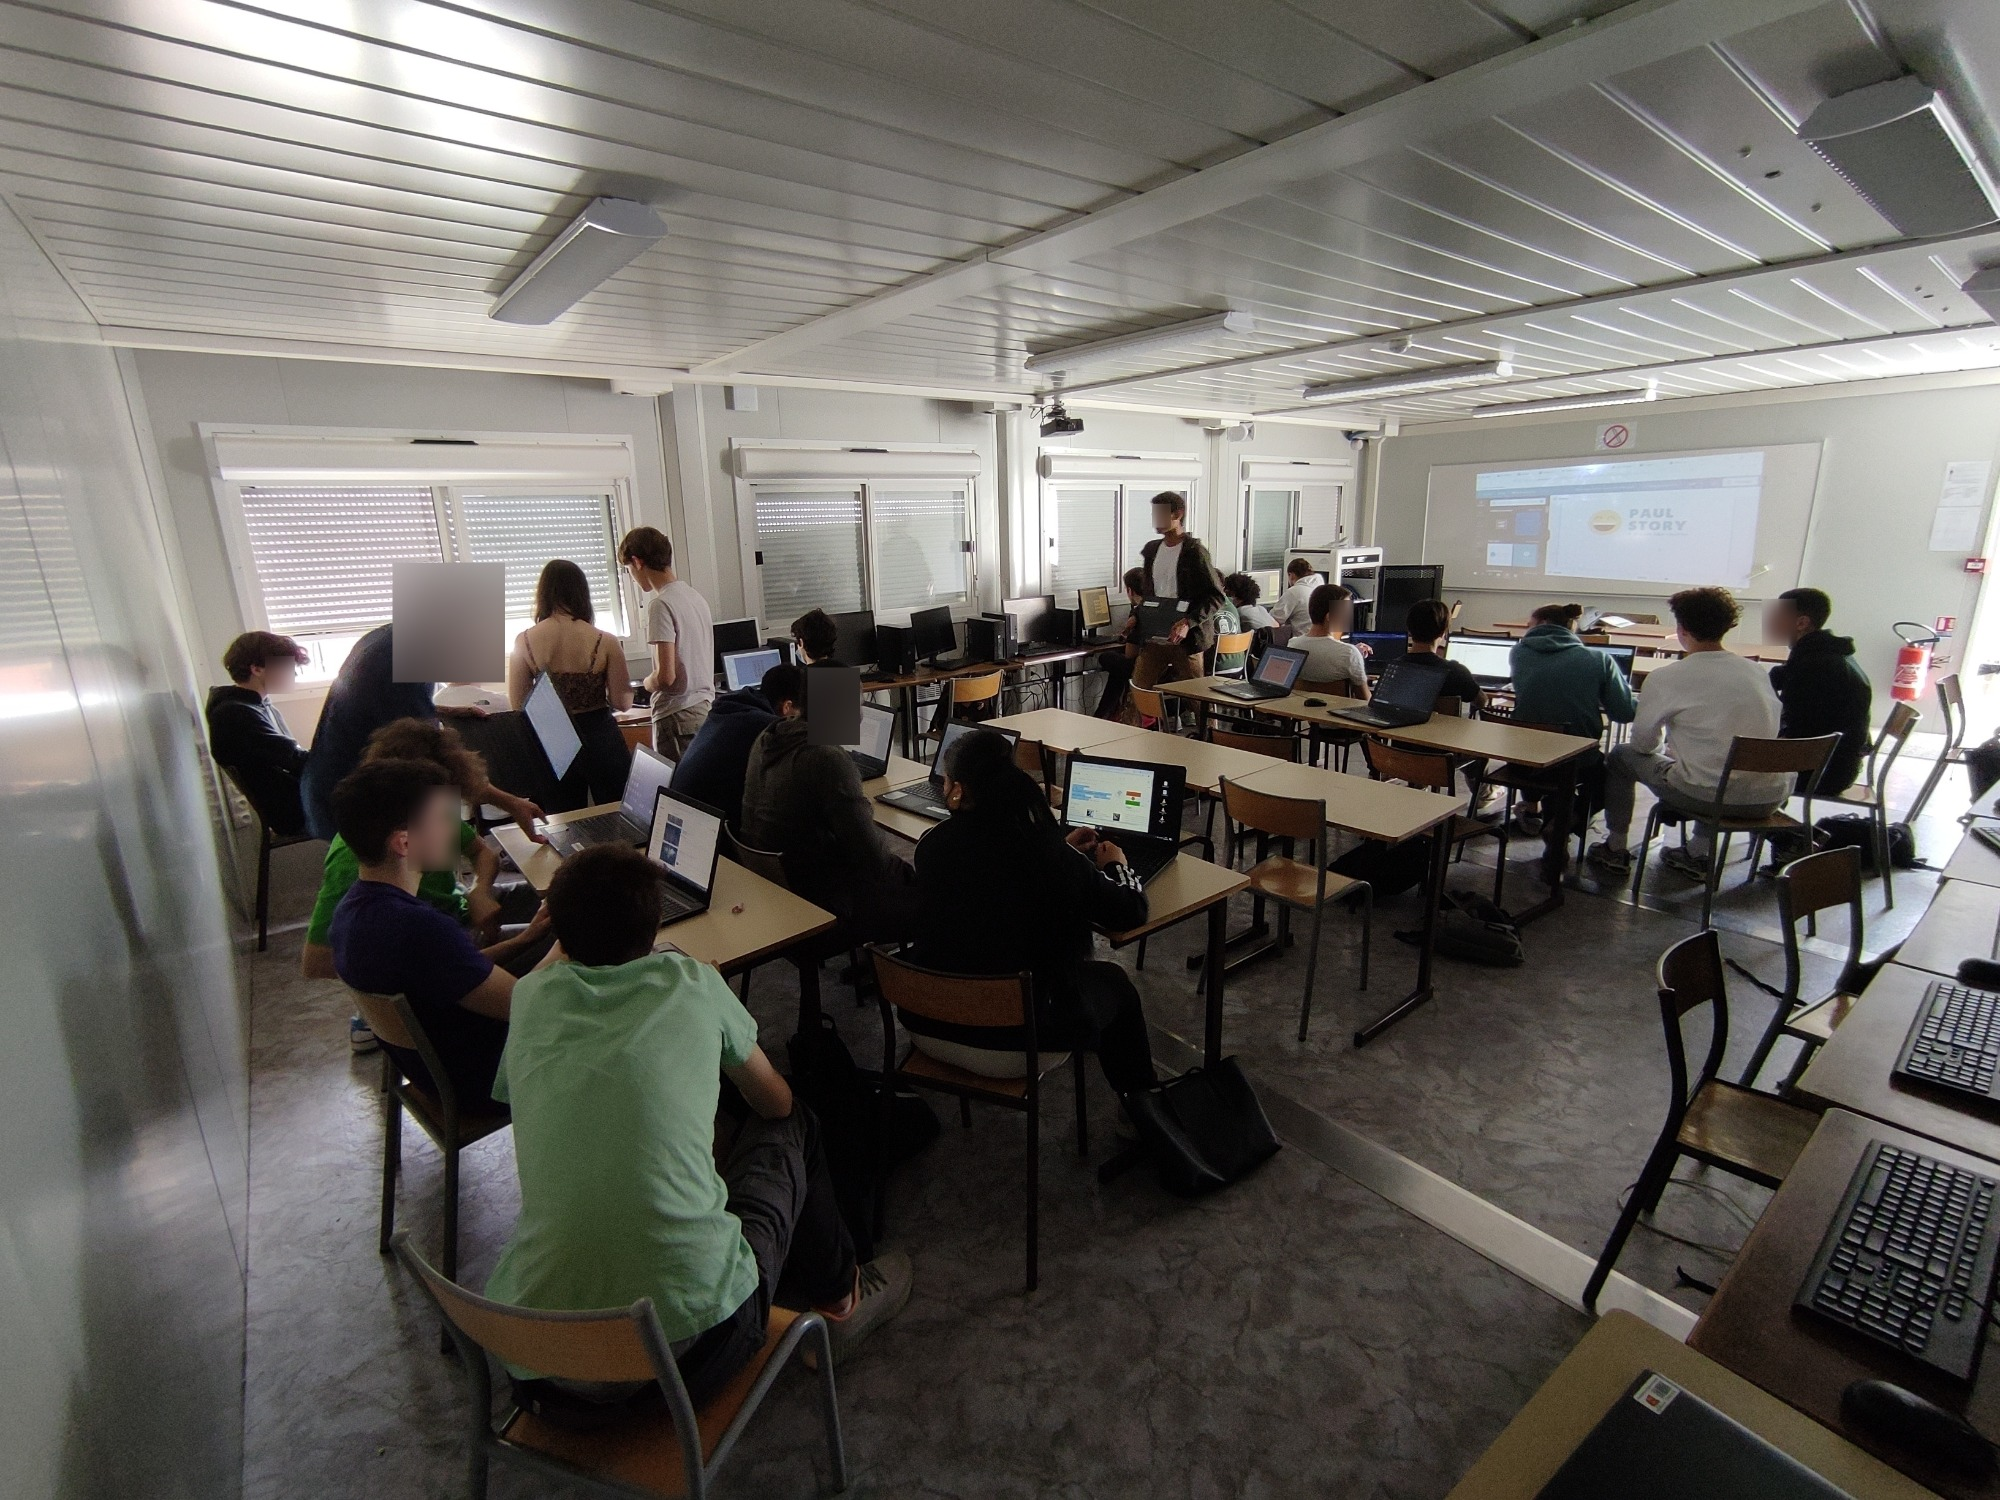
\includegraphics[width=0.8\textwidth]{annexes/pedagogiques/productions/jeux-photo-etudiants (1).jpg}
    \caption{Équipes interdisciplinaires en session de travail collaboratif (visages floutés pour l'anonymat).}
    \label{fig-equipes-travail-1}
\end{figure}

\subsection{Le défi humain : recruter et fédérer dans un contexte difficile}

Le recrutement des collègues a été particulièrement difficile dans un lycée d'élite où la culture de la collaboration bénévole était peu présente et où les emplois du temps étaient déjà très chargés.

\subsubsection{Stratégies de mobilisation développées}

\begin{enumerate}[leftmargin=*]
    \item \textbf{Communication ciblée} : présentation individualisée du projet à chaque collègue potentiel, en mettant en avant les bénéfices pour sa discipline
    \item \textbf{Limitation de l'engagement} : proposition d'un cadre horaire raisonnable (4 séances de 2h par enseignant)
    \item \textbf{Soutien institutionnel} : appui de ma tutrice INSPÉ auprès de la direction pour valoriser le projet
    \item \textbf{Valorisation des productions} : engagement à présenter le jeu dans chaque classe participante
\end{enumerate}

Cette expérience illustre la compétence \textbf{« Situer ses interventions dans un écosystème professionnel »} du référentiel MEEF \parencite{rncp38152}, compétence qui ne se limite pas à collaborer ponctuellement mais implique de créer et d'animer une dynamique collective \parencite{competences_transversales_eurecia}.

\subsection{Management de projet agile adapté au contexte scolaire}

J'ai adopté une posture de \textbf{tuteur-cadre} plutôt que de chef de projet direct, inspirée des méthodes agiles Scrum \parencite{scrum_education}. Cette approche développe l'autonomie des élèves dans la gestion de leur projet.

\subsubsection{Structure de management mise en place}

\begin{itemize}[leftmargin=*]
    \item \textbf{Réunions de lancement} : définition collective des objectifs, du planning et des rôles
    \item \textbf{Sprints de 2 semaines} : cycles de travail avec objectifs précis
    \item \textbf{Stand-up meetings} : points réguliers de 15 minutes en fin de séance
    \item \textbf{Rétrospectives} : bilans collectifs après chaque sprint pour ajuster l'organisation
    \item \textbf{Outils collaboratifs} : utilisation de Trello pour la gestion des tâches et de GitLab pour le versionnage du code
\end{itemize}

Cette organisation responsabilise les élèves et leur permet de développer des compétences de gestion de projet directement transférables au monde professionnel \parencite{projet_travail_groupe}.

\section{Axe 3 : Déroulement et défis rencontrés}

\subsection{Chronologie du projet}

\textbf{Septembre - Octobre} : Conception du moteur de jeu et recrutement des équipes\\
\textbf{Novembre - Décembre} : Premier sprint (définition du scénario, premiers graphismes)\\
\textbf{Janvier - Février} : Deuxième sprint (développement des niveaux, musiques)\\
\textbf{Mars - Avril} : Troisième sprint (traductions, tests, corrections)\\
\textbf{Mai} : Finalisation et présentation aux classes participantes

\subsection{Gestion réaliste des contraintes}

Comme tout projet ambitieux, celui-ci a connu plusieurs défis \parencite{projet_travail_groupe,competences_transversales} :

\subsubsection{Dépassement des délais initiaux}
Le planning initial prévoyait une finalisation en mars, mais des difficultés techniques (bugs complexes, incompatibilités entre modules) et organisationnelles (absences, examens blancs) ont imposé un report à mai. Cette gestion de l'imprévu a nécessité :
\begin{itemize}[leftmargin=*]
    \item Une repriorisation des fonctionnalités (abandon de certaines fonctionnalités secondaires)
    \item Une réorganisation du planning avec des séances de travail supplémentaires volontaires
    \item Une communication transparente avec tous les acteurs sur les ajustements nécessaires
\end{itemize}

\subsubsection{Fluctuation de l'implication}
Certains membres se sont moins investis que d'autres, nécessitant des interventions de médiation et de remotivation. Ces compétences de management relationnel, développées en entreprise \parencite{knowles_andragogy}, se sont révélées directement transférables au contexte pédagogique.



\section{Axe 4 : Résultats et Analyse Réflexive}

\subsection{Bilan des productions et impacts}

\subsubsection{Un produit fini complet et professionnel}

Le résultat final est un jeu de type Zelda 2D, fonctionnel et riche, comprenant \parencite{pygame_tutorial} :

\begin{itemize}[leftmargin=*]
    \item \textbf{4 niveaux jouables} avec difficulté progressive
    \item \textbf{Un scénario à message positif} : « La rédemption d'un homme riche » (thématique sociale proposée par les élèves)
    \item \textbf{Des énigmes variées} : logique, exploration, résolution de problèmes
    \item \textbf{Des objets à collecter} et un système d'inventaire
    \item \textbf{Des PNJ avec dialogues} contextuels et aide au joueur
    \item \textbf{Une bande sonore originale} composée spécifiquement pour le jeu
    \item \textbf{Une interface multilingue} (français, anglais, italien)
    \item \textbf{Un système de sauvegarde} permettant de reprendre la partie
\end{itemize}

\begin{figure}[H]
    \centering
    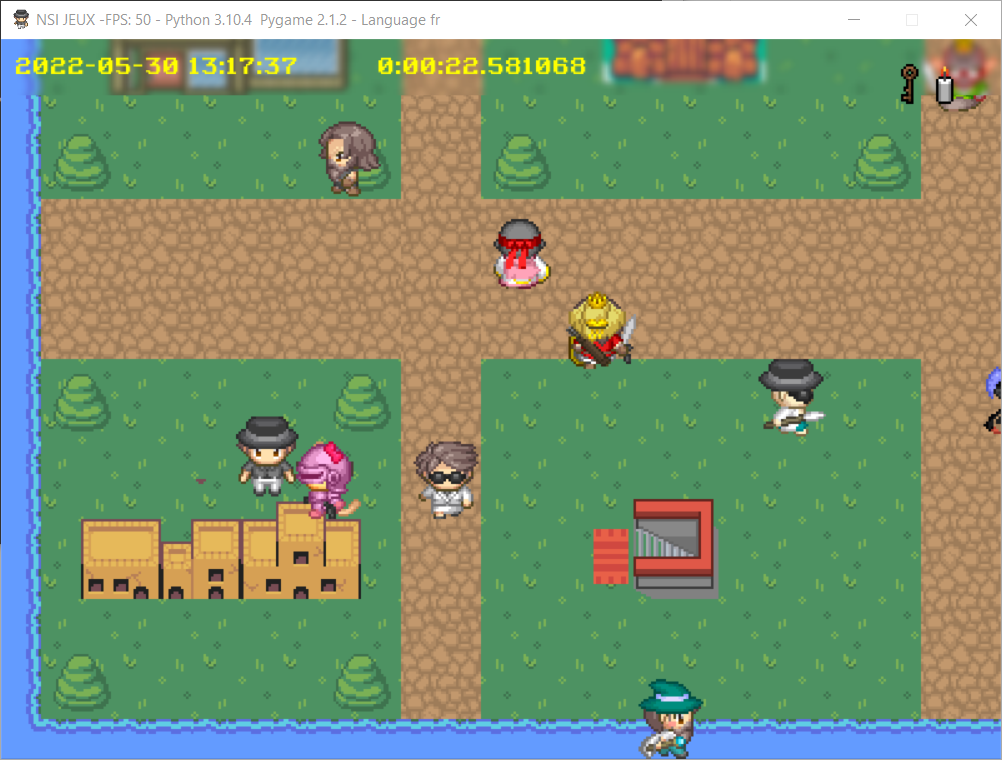
\includegraphics[width=0.8\textwidth]{annexes/pedagogiques/productions/jeux-capture-ecran (1).png}
    \caption{Interface principale du jeu développé collectivement.}
    \label{fig-jeu-menu}
\end{figure}

\begin{figure}[H]
    \centering
    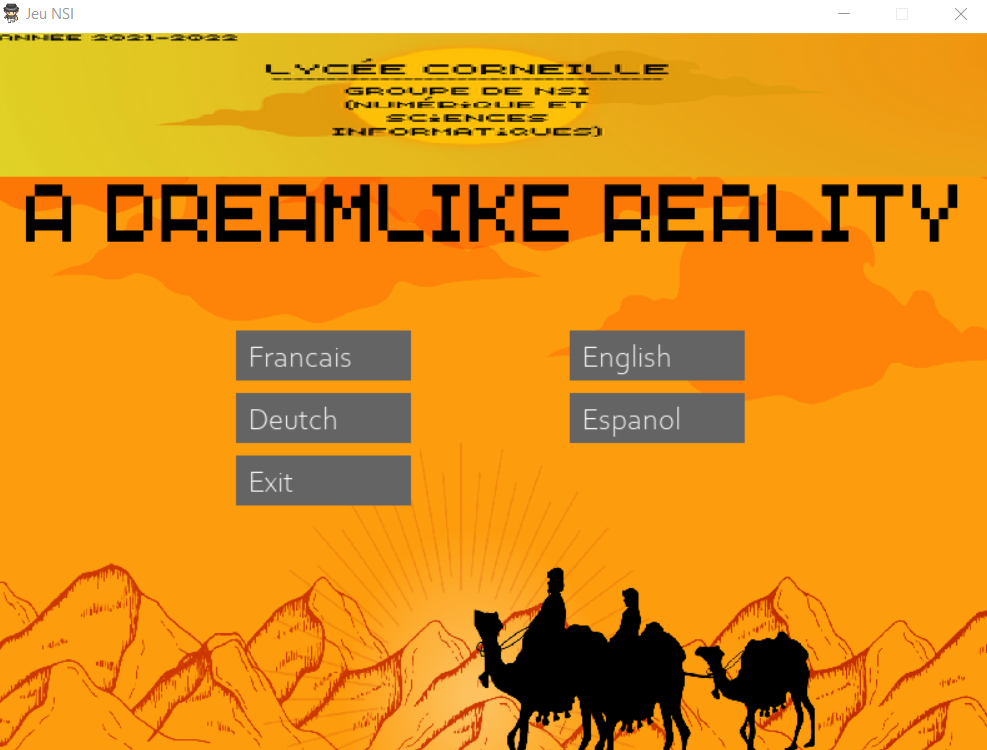
\includegraphics[width=0.8\textwidth]{annexes/pedagogiques/productions/jeux-capture-ecran (2).png}
    \caption{Exemple de niveau de jeu avec l'interface utilisateur.}
    \label{fig-jeu-niveau}
\end{figure}

\subsubsection{Impact au-delà de la classe}

Le projet a eu un rayonnement significatif \parencite{pedagogie_active} :

\begin{enumerate}[leftmargin=*]
    \item \textbf{Démonstrations dans les classes} : présentation du jeu dans toutes les classes des enseignants participants, valorisant le travail des élèves
    \item \textbf{Présentation en conseil pédagogique} : le projet a été présenté comme exemple de collaboration interdisciplinaire
    \item \textbf{Article dans le journal du lycée} : mise en valeur du travail collectif
    \item \textbf{Mise à disposition du jeu} : téléchargement possible sur la Forge des Communs Numériques Éducatifs \parencite{forge_educative}
\end{enumerate}

\subsubsection{Développement de compétences transversales}

L'évaluation qualitative post-projet révèle des acquis significatifs \parencite{competences_transversales_eurecia} :

\begin{itemize}[leftmargin=*]
    \item \textbf{Compétences techniques NSI} : Tous les élèves de l'équipe coordinatrice ont validé les compétences du programme relatives à la POO et à la gestion de projet
    \item \textbf{Compétences collaboratives} : 85\% des élèves déclarent avoir développé leur capacité à travailler en équipe interdisciplinaire
    \item \textbf{Autonomie et initiative} : 90\% des élèves déclarent avoir pris des initiatives personnelles dans le projet
    \item \textbf{Gestion du temps} : 75\% déclarent avoir amélioré leur capacité à respecter des délais
\end{itemize}

\subsubsection{Modalités d'évaluation}
L'évaluation du projet s'est appuyée sur une grille critériée permettant d'apprécier à la fois les compétences techniques et les compétences transversales.

\begin{longtable}{|p{3.5cm}|p{2.5cm}|p{2.5cm}|p{2.5cm}|p{2.5cm}|}
\caption{Grille d'évaluation Projet Collaboratif Interdisciplinaire - Jeu Vidéo} \\
\hline
\textbf{Compétences} & \textbf{Non acquis (0-7)} & \textbf{En cours (8-12)} & \textbf{Acquis (13-16)} & \textbf{Maîtrisé (17-20)} \\
\hline
\endfirsthead
\hline
\textbf{Compétences} & \textbf{Non acquis (0-7)} & \textbf{En cours (8-12)} & \textbf{Acquis (13-16)} & \textbf{Maîtrisé (17-20)} \\
\hline
\endhead

\textbf{Programmation Python/Pygame} &
Code non fonctionnel, erreurs majeures &
Code partiellement fonctionnel &
Code fonctionnel et structuré &
Code optimisé, commenté, élégant \\
\hline

\textbf{Collaboration interdisciplinaire} &
Travail en silo, pas d'échanges &
Échanges ponctuels &
Collaboration effective régulière &
Synergie créative, leadership \\
\hline

\textbf{Gestion de projet} &
Pas de planification &
Planning basique suivi &
Gestion efficace des tâches &
Méthodes agiles maîtrisées \\
\hline

\textbf{Intégration des 5 disciplines} &
Une seule discipline intégrée &
2-3 disciplines présentes &
4-5 disciplines harmonieusement intégrées &
Synergie exceptionnelle entre toutes les disciplines \\
\hline

\end{longtable}

\subsection{Analyse réflexive approfondie}

\subsubsection{Analyse a priori : Le pari de l'interdisciplinarité}
Mon intention pédagogique initiale reposait sur le postulat que le \textbf{jeu vidéo} agirait comme un "objet-frontière" \parencite{star_griesemer_boundary_objects}, capable de fédérer des disciplines cloisonnées (Arts, Langues, Histoire, Info). Je faisais l'hypothèse que :
\begin{itemize}
    \item La motivation intrinsèque pour le jeu vidéo compenserait la difficulté de la coordination.
    \item Les élèves développeraient naturellement des compétences de communication pour faire dialoguer leurs expertises respectives.
    \item Le rôle de "tuteur-cadre" suffirait à maintenir la cohésion sans interventionnisme excessif.
\end{itemize}

\subsubsection{Analyse a posteriori : La réalité du terrain}
L'expérience a validé la puissance motivationnelle du support, mais a révélé que la \textbf{collaboration ne se décrète pas}, elle s'apprend. J'ai observé que sans une structuration très forte (les rituels agiles), les groupes tendaient naturellement à travailler en silos (les graphistes font des dessins, les codeurs codent, sans se parler). La "magie" de l'interdisciplinarité n'a opéré que parce qu'elle a été provoquée et maintenue par une ingénierie de projet rigoureuse.

\subsubsection{Difficultés imprévues et régulations (Analyse Multi-agenda)}
La gestion de ce projet a nécessité une régulation fine de mon activité, analysable via le \textbf{multi-agenda de Bucheton} \parencite{bucheton_postures}. J'ai dû gérer simultanément des préoccupations parfois contradictoires :

\begin{itemize}[leftmargin=*]
    \item \textbf{Pilotage et Chronogenèse} : Contrairement à un cours magistral, le pilotage s'est fait « à vue ». J'ai dû accepter de relâcher le contrôle temporel strict pour m'adapter au rythme d'avancement disparate des groupes, acceptant que tous n'atteignent pas le même point au même moment.
    \item \textbf{Atmosphère et Tissage} : L'enjeu était de maintenir une atmosphère de travail collaboratif (bruit productif) tout en évitant la dispersion. Le tissage s'est opéré en reliant constamment leurs problèmes techniques immédiats (« mon personnage ne saute pas ») aux concepts théoriques vus en cours (« c'est une question de vecteur vitesse »).
    \item \textbf{Étayage et Postures} : Ma posture dominante a glissé du \textbf{contrôle} (au début) à l'\textbf{accompagnement} et au \textbf{lâcher-prise}. J'ai agi comme une « personne ressource », intervenant à la demande pour débloquer une situation (étayage local) plutôt que pour diriger l'action (étayage global).
\end{itemize}

Face aux obstacles spécifiques :
\begin{itemize}[leftmargin=*]
    \item \textbf{Hétérogénéité technique} : L'écart de niveau NSI 1ère/Terminale a menacé de bloquer le développement.
    \item \textbf{Solution} : Mise en place de "binômes de compétences" (tutorat par les pairs) et création de modules de code "prêts à l'emploi" pour les novices.
    
    \item \textbf{Tensions interpersonnelles} : Des conflits de leadership sont apparus.
    \item \textbf{Solution} : Médiation active et rappel des rôles définis par la charte de projet initiale.
    
    \item \textbf{Essoufflement de la motivation} : Baisse de régime au milieu du 2ème trimestre.
    \item \textbf{Solution} : Organisation d'une "démo intermédiaire" valorisante devant le Proviseur pour relancer la dynamique.
\end{itemize}

\subsubsection{Axes d'amélioration}
Pour une future itération, je proposerais :
\begin{itemize}
    \item \textbf{Une échelle plus réduite} : Commencer par un "Game Jam" de 48h pour souder les équipes avant le projet long.
    \item \textbf{Des outils de communication unifiés} : Imposer un seul canal (ex: Discord éducatif ou Teams) pour éviter la dispersion de l'information.
    \item \textbf{Une évaluation par les pairs formalisée} : Intégrer plus tôt la méthode de "notation à l'enveloppe" (voir Expérience 3) pour réguler l'investissement individuel.
\end{itemize}

\subsection{Transférabilité et compétences MEEF validées}

Cette expérience valide plusieurs blocs du référentiel RNCP38152 \parencite{rncp38152} à un niveau expert :

\subsubsection{BC09 - Acteur de la communauté éducative}

Je n'ai pas seulement collaboré, j'ai \textbf{initié et construit} une collaboration interdisciplinaire dans un environnement a priori peu favorable. Mobiliser des collègues agrégés de disciplines variées autour d'un projet numérique démontre des compétences avancées de :
\begin{itemize}[leftmargin=*]
    \item Leadership pédagogique
    \item Communication institutionnelle
    \item Diplomatie et négociation
    \item Animation d'une communauté éducative \parencite{competences_transversales}
\end{itemize}

\subsubsection{BC05 - Didactique de l'informatique et pédagogie de projet}

Cette expérience est un cas d'école de la pédagogie de projet \parencite{kilpatrick_project_method,dewey_experience_education,projet_methode_tlem}. Les notions techniques de NSI ne sont pas apprises hors-sol, mais au service d'un but créatif et motivant. La création du moteur de jeu constitue une forme avancée de transposition didactique : rendre appropriable par des lycéens un système informatique complexe \parencite{chevallard_transposition}.

\subsubsection{BC04 - Conduite de projet et recherche-action}

La démarche suivie (Analyse du problème → Conception d'une solution → Mise en œuvre → Analyse des résultats) est celle d'un praticien-chercheur \parencite{schon_reflective_practitioner,recherche_action_education}. Cette recherche-action illustre la conduite autonome d'un projet pédagogique complexe.

\subsubsection{BC06 - Praticien réflexif}

Mon rôle de tuteur-cadre et la mise en place d'une structure de management inspirée des méthodes agiles montrent que ma réflexion portait sur l'\textbf{organisation de l'apprentissage elle-même} \parencite{perrenoud_pratique_reflexive}, développant chez les élèves des compétences de gestion de projet essentielles pour leur future vie professionnelle \parencite{competences_transversales,scrum_education}.

\subsection{Perspectives de recherche}

Cette expérience nourrit directement mon projet de thèse sur plusieurs aspects \parencite{intelligence_artificielle_education} :

\begin{enumerate}[leftmargin=*]
    \item \textbf{IA et différenciation} : Comment l'IA pourrait-elle aider à adapter automatiquement les tâches du projet au niveau de chaque élève ?
    \item \textbf{Évaluation des compétences transversales} : Comment mesurer objectivement le développement des soft skills dans un projet collaboratif ?
    \item \textbf{Collaboration numérique} : Quels outils numériques optimisent la collaboration interdisciplinaire en contexte scolaire ?
\end{enumerate}

\chapter{Expérience 3 : Ingénierie de l'évaluation - La « Notation à l'Enveloppe » (Méthode Italienne)}

\section{Axe 1 : Intentions pédagogiques et fondements éthiques}

\subsection{Genèse et conception originale : la « Notation à l'Enveloppe »}

Le dispositif d'évaluation appelé \textbf{« Notation à l'Enveloppe »} (surnommé informellement « Méthode Italienne » en référence à une expérience personnelle de Gentil Organisateur en hôtel-club en Sicile, où l'équipe recevait une enveloppe globale de pourboires et gratifications à répartir de manière concertée entre animateurs selon l'engagement de chacun) est une ingénierie d'évaluation originale que j'ai transposée dans le champ pédagogique pour répondre aux écueils de la notation de groupe indifférenciée.

Ayant développé ce protocole de manière empirique pour résoudre la problématique d'équité identifiée lors des projets collaboratifs (notamment à la suite de l'Expérience 2), j'ai ensuite entrepris une recherche approfondie dans la littérature didactique pour en analyser la portée. J'ai alors constaté avec un grand intérêt que des équipes universitaires et chercheurs avaient expérimenté des démarches d'évaluation par les pairs fortement convergentes :
\begin{itemize}[leftmargin=*]
    \item \textbf{À l'UTC Compiègne et à l'Université de Poitiers} \parencite{evaluation_pairs_utc,evaluation_pairs_univ_poitiers}, des enseignants-chercheurs ont conçu des systèmes d'allocation de points intra-groupe pour responsabiliser les étudiants et mesurer la contribution réelle au projet.
    \item \textbf{Dans la recherche internationale sur le Peer Assessment} \parencite{topping_peer_assessment,scallon_evaluation}, des travaux théorisent le rôle de l'évaluation par les pairs dans la construction de l'auto-régulation et du sentiment de justice redistributive.
\end{itemize}

Cette convergence entre mon intuition pédagogique de terrain et les travaux de recherche universitaires confirme la pertinence et la transférabilité de cette ingénierie d'évaluation régulatrice.

\subsection{Problématique d'ingénierie d'évaluation et double constat}

Le développement de cette méthode répond à deux défis majeurs en ingénierie de formation :
\begin{enumerate}[leftmargin=*]
    \item \textbf{Le risque d'injustice redistributive} : L'attribution d'une note unique globale occulte les écarts d'investissement individuel, générant de la frustration chez les apprenants moteurs et un risque de déresponsabilisation.
    \item \textbf{Les limites de l'observation magistrale directe} : Dans des dispositifs de pédagogie active (projets en sous-groupes), le formateur ou enseignant ne peut appréhender seul la dynamique fine des interactions et la répartition effective des charges de travail.
\end{enumerate}

Cette expérimentation s'inscrit donc au cœur des compétences du Master MEEF PIF / FFMS : l'\textbf{ingénierie des dispositifs d'évaluation régulatrice} \parencite{perrenoud_pratique_reflexive,nicol_formative_assessment}, visant à transformer l'évaluation sommative subie en un vecteur d'auto-régulation, de métacognition et d'apprentissage sociocognitif.

\subsection{Le prérequis : maturité du groupe-classe}

Ce système n'est pas applicable à n'importe quelle classe. Il nécessite deux conditions préalables \parencite{evaluation_pairs_utc} :

\begin{itemize}[leftmargin=*]
    \item \textbf{Connaissance mutuelle} : Les élèves doivent se connaître suffisamment pour évaluer objectivement le travail de leurs pairs
    \item \textbf{Maturité collective} : Il doit exister une certaine confiance et une culture de l'honnêteté au sein du groupe-classe pour que le processus soit sain et constructif
\end{itemize}

Pour ces raisons, je ne mets en place cette méthode qu'à partir du \textbf{second semestre de première NSI}, après plusieurs mois de travail collectif ayant permis de développer cette maturité.

\subsection{Les objectifs pédagogiques implicites}

Au-delà de l'évaluation sommative, cette méthode vise plusieurs objectifs formatifs essentiels \parencite{perrenoud_pratique_reflexive} :

\subsubsection{Développer la métacognition}

Amener les élèves à réfléchir sur :
\begin{itemize}[leftmargin=*]
    \item Leur propre contribution au projet (auto-évaluation)
    \item La contribution des autres membres (évaluation par les pairs) \parencite{evaluation_pairs_univ_poitiers}
    \item Les critères d'une contribution de qualité (construction d'une grille d'évaluation mentale)
\end{itemize}

Cette dimension métacognitive est reconnue comme essentielle pour le développement de l'autonomie et de la pratique réflexive \parencite{perrenoud_pratique_reflexive,schon_reflective_practitioner}, et elle s'appuie sur les principes de l'évaluation formative et de l'auto-régulation des apprentissages \parencite{nicol_formative_assessment,topping_peer_assessment}.

\subsubsection{Enseigner la responsabilité}

Chaque membre est responsable non seulement de sa propre note, mais aussi de l'impact de son travail (ou de son absence de travail) sur le groupe. Cette responsabilisation développe une conscience professionnelle transférable au monde du travail \parencite{competences_transversales}.

\subsubsection{Former au management équitable}

Les chefs de projet sont initiés à la difficile tâche d'évaluer le travail de leurs pairs de manière juste et argumentée. Cette compétence managérial est rarement enseignée au lycée mais constitue un atout majeur pour leur future carrière \parencite{knowles_andragogy}.

\section{Axe 2 : Déroulement méthodologique en 5 étapes structurées}

La méthode de « Notation à l'Enveloppe » suit un protocole rigoureux en 5 étapes, garantissant à la fois l'équité du processus et l'acceptation du résultat par les élèves.

\subsection{Étape 1 : Présentation transparente des règles du jeu}

Lors de la présentation du premier projet de groupe de l'année, j'explique clairement et précisément le système d'évaluation \parencite{evaluation_pairs_utc} :

\begin{itemize}[leftmargin=*]
    \item \textbf{Principe fondamental} : La note de groupe sera distribuée entre les membres selon leur contribution effective
    \item \textbf{Rôle du chef de projet} : Il sera responsable de proposer la répartition des points, non pas en tant que "juge" mais en tant que "témoin privilégié" du travail de chacun
    \item \textbf{Mécanisme de validation} : Toutes les propositions seront discutées collectivement entre chefs de projet sous ma supervision
    \item \textbf{Objectifs pédagogiques} : Développer la responsabilité individuelle, la justice dans le travail collaboratif et la capacité d'auto-évaluation
\end{itemize}

Cette transparence initiale génère une compréhension et une adhésion des élèves, condition sine qua non du succès de la méthode.

\subsection{Étape 2 : Attribution d'un projet de groupe structuré}

Le projet assigné doit présenter certaines caractéristiques pour que la méthode soit pertinente :

\begin{itemize}[leftmargin=*]
    \item \textbf{Durée suffisante} : Au minimum 3 semaines pour permettre l'observation des contributions sur la durée
    \item \textbf{Tâches diversifiées} : Mélange de recherche, conception, réalisation technique, présentation orale
    \item \textbf{Interdépendance des rôles} : Chaque membre doit avoir une contribution identifiable mais complémentaire
    \item \textbf{Groupes de 3 à 4 élèves maximum} : Au-delà, l'évaluation par les pairs devient trop complexe
\end{itemize}

Observation significative : lors de la désignation des chefs de projet, les groupes choisissent leurs chefs en fonction de leur fiabilité plutôt que de leur popularité. Cette dynamique montre que le système répond à un besoin de justice ressenti par les élèves eux-mêmes \parencite{evaluation_pairs_univ_poitiers}.

\subsection{Étape 3 : Calcul et attribution du "capital points" à distribuer}

À l'issue du projet, j'évalue le travail collectif du groupe et attribue une note globale (par exemple : 12/20). Cette note génère un \textbf{"capital points"} que le chef de projet devra répartir.

\subsubsection{Exemple concret de calcul}

Pour un groupe de 3 élèves ayant obtenu 12/20 :
\begin{itemize}[leftmargin=*]
    \item \textbf{Capital total} : 12 × 3 = 36 points à distribuer
    \item \textbf{Contrainte} : La somme des notes individuelles doit égaler exactement 36 points
    \item \textbf{Amplitude possible} : Les notes peuvent varier de 8/20 à 16/20 environ (selon les cas)
\end{itemize}

Cette contrainte mathématique simple garantit que l'évaluation reste dans des proportions raisonnables tout en permettant une réelle différenciation.

\subsection{Étape 4 : Répartition interne par le chef de projet}

Le chef de projet dispose d'une \textbf{grille d'évaluation simplifiée} pour objectiver sa proposition \parencite{evaluation_formative}. Cette grille se concentre sur quatre critères principaux :

\begin{enumerate}[leftmargin=*]
    \item \textbf{Assiduité et ponctualité} : Présence effective aux séances de travail en groupe
    \item \textbf{Qualité des contributions} : Pertinence et finition du travail produit
    \item \textbf{Respect des délais} : Livraison des tâches assignées dans les temps convenus
    \item \textbf{Esprit collaboratif} : Entraide, communication constructive, gestion des conflits
\end{enumerate}

\subsubsection{Processus de réflexion guidé}

Le chef de projet doit :
\begin{itemize}[leftmargin=*]
    \item \textbf{Auto-évaluer} sa propre contribution en premier
    \item \textbf{Justifier} chaque attribution par des faits observables
    \item \textbf{Proposer} une répartition équitable en points entiers
    \item \textbf{Anticiper} les possibles contestations et préparer ses arguments
\end{itemize}

Cette étape développe des compétences managériales et d'analyse objective cruciales pour la suite de leur parcours.

\subsection{Étape 5 : "Table Ronde" de validation collective (Analyse des Postures)}

La réunion finale constitue le moment pédagogique le plus riche. Analysée à travers le modèle de \textbf{l'ajustement pédagogique} d'Éric Saillot et des postures de Bucheton \parencite{saillot_ajustement,bucheton_postures}, cette phase illustre la complexité de l'étayage enseignant.

Je ne suis pas simplement un "modérateur", je construis une \textbf{posture d'ajustement} systémique articulant le "penser-dire-faire", en naviguant entre trois postures clés :

\begin{itemize}[leftmargin=*]
    \item \textbf{Posture d'accompagnement (Aide latérale)} : C'est ma posture dominante. Je suis assis \textit{avec} les élèves, pas \textit{face} à eux. J'écoute, je reformule leurs arguments ("Si je comprends bien, tu valorises son effort plus que son résultat ?"), aidant à expliciter leur pensée sans imposer la mienne.

    \item \textbf{Posture de contrôle (Cadrage serré)} : J'active cette posture instantanément si l'éthique est menacée (ex: règlement de compte personnel, discrimination). Je deviens alors le garant des règles du jeu et de la sécurité psychologique de chacun ("Stop, cet argument n'est pas recevable car il ne porte pas sur le travail").

    \item \textbf{Posture de lâcher-prise (Autonomie confiée)} : À certains moments, je me mets volontairement en retrait ("Et vous, les autres chefs, qu'en pensez-vous ?") pour laisser la régulation sociale opérer. C'est le moment où la compétence s'incarne véritablement chez les élèves.
\end{itemize}

Cette flexibilité posturale permet de transformer une simple réunion administrative en un véritable espace de développement professionnel pour les élèves.

\section{Axe 3 : Résultats observés et impacts}

\subsection{Analyse du Multi-agenda (Bucheton) sur l'ensemble de la séquence}

Pour compléter cette analyse, je peux lire l'ensemble de ce dispositif à travers les cinq préoccupations du \textbf{multi-agenda} \parencite{bucheton_postures} :
\begin{itemize}[leftmargin=*]
    \item \textbf{Pilotage} : Le dispositif est très structuré (étapes, grilles, capital points) pour éviter la dérive "subjective".
    \item \textbf{Atmosphère} : L'enjeu est de maintenir un climat de confiance et de justice ("ethos").
    \item \textbf{Tissage} : Je relie constamment leur expérience immédiate (noter un camarade) à des enjeux professionnels (évaluation annuelle, travail d'équipe).
    \item \textbf{Étayage} : Je fournis les outils (la grille) pour qu'ils puissent réussir la tâche complexe d'évaluation.
    \item \textbf{Objets de savoir} : L'objet n'est plus le code informatique, mais la compétence métacognitive d'évaluation elle-même.
\end{itemize}

\subsection{Une différenciation modérée et acceptée}

\subsubsection{Données quantitatives}

Sur 5 ans d'utilisation de cette méthode, j'observe des écarts modérés et acceptés \parencite{evaluation_pairs_univ_poitiers}, révélant l'équité du processus.

\subsubsection{Acceptation qualitative}

La majorité des élèves \textbf{comprennent et acceptent leur note}, même lorsqu'elle est inférieure à celle du groupe. Cette acceptation s'explique par la transparence du processus et la légitimité du chef de projet \parencite{evaluation_formative}.

\subsection{Un leadership basé sur la fiabilité plutôt que sur la popularité}

Les élèves comprennent rapidement que choisir un chef « copain » mais peu fiable conduit à un résultat médiocre. Ils développent donc une approche plus pragmatique du choix de leur chef, valorisant la \textbf{fiabilité} et la \textbf{capacité d'organisation} \parencite{competences_transversales}.

\subsection{Impact puissant sur la motivation et l'inclusion}

Le système agit comme un outil de diagnostic et de motivation \parencite{pedagogie_active}, permettant à chaque élève de se sentir reconnu pour sa contribution.



\subsection{Matériels produits}

Pour soutenir cette démarche, j'ai conçu et mis à jour la fiche d'évaluation distribuée aux apprenants (\textbf{document original joint au format PDF :} \url{sources/grille.pdf}, également reproduit dans les Annexes). Ces outils constituent une ingénierie d'évaluation opérationnelle, affinée sur le terrain et transférable à d'autres dispositifs de formation par projet.

\subsubsection{Principe de la notation à l'enveloppe}
L'évaluation repose sur le principe de la "notation à l'italienne" :
\begin{itemize}
    \item L'enseignant attribue une \textbf{enveloppe globale de points} au groupe, basée sur sa grille d'évaluation du projet.
    \item Les étudiants (pairs) proposent une \textbf{répartition de ces points} entre eux, en fonction de l'implication individuelle de chacun.
\end{itemize}

Il n'y a donc pas de pondération fixe, mais une distribution dynamique des points alloués au collectif.

\subsubsection{Grille d'évaluation professorale}
Cette grille me permet d'évaluer le produit fini rendu par le groupe et de déterminer l'enveloppe de points à distribuer.

\begin{longtable}{|p{4cm}|p{2cm}|p{2cm}|p{2cm}|p{2cm}|p{2cm}|}
\caption{Grille d'évaluation "à l'italienne" - Évaluation professorale} \\
\hline
\textbf{Critères projet} & \textbf{Insuffisant (0-4)} & \textbf{Fragile (5-8)} & \textbf{Satisfaisant (9-12)} & \textbf{Très bien (13-16)} & \textbf{Excellent (17-20)} \\
\hline
\endfirsthead
\hline
\textbf{Critères projet} & \textbf{Insuffisant (0-4)} & \textbf{Fragile (5-8)} & \textbf{Satisfaisant (9-12)} & \textbf{Très bien (13-16)} & \textbf{Excellent (17-20)} \\
\hline
\endhead
\textbf{Qualité technique} &
Produit non fonctionnel &
Fonctionnalités basiques &
Produit fonctionnel stable &
Qualité technique élevée &
Excellence technique \\
\hline
\textbf{Innovation et créativité} &
Aucune originalité &
Quelques éléments originaux &
Approche créative &
Solutions innovantes &
Innovation remarquable \\
\hline
\textbf{Respect des contraintes} &
Contraintes ignorées &
Respect partiel &
Contraintes respectées &
Dépassement des attentes &
Excellence dans les contraintes \\
\hline
\textbf{Documentation} &
Aucune documentation &
Documentation minimale &
Documentation correcte &
Documentation complète &
Documentation exemplaire \\
\hline
\end{longtable}

\subsubsection{Grille d'évaluation par les pairs}
Cette grille est utilisée par le chef de projet pour évaluer l'implication de chaque membre.

\begin{longtable}{|p{4cm}|p{3cm}|p{3cm}|p{3cm}|p{3cm}|}
\caption{Grille d'évaluation "à l'italienne" - Évaluation par les pairs} \\
\hline
\textbf{Critères implication} & \textbf{Passif (0-5)} & \textbf{Ponctuel (6-10)} & \textbf{Actif (11-15)} & \textbf{Leader (16-20)} \\
\hline
\endfirsthead
\hline
\textbf{Critères implication} & \textbf{Passif (0-5)} & \textbf{Ponctuel (6-10)} & \textbf{Actif (11-15)} & \textbf{Leader (16-20)} \\
\hline
\endhead
\textbf{Participation aux réunions} &
Absent ou silencieux &
Présent mais peu participatif &
Participation régulière &
Animation et leadership \\
\hline
\textbf{Contribution technique} &
Aucune contribution &
Contributions mineures &
Contributions significatives &
Contributions clés et expertises \\
\hline
\textbf{Esprit d'équipe} &
Individualiste, conflits &
Coopération minimale &
Bon esprit d'équipe &
Moteur de l'équipe \\
\hline
\textbf{Respect des délais} &
Retards systématiques &
Quelques retards &
Ponctualité respectée &
Anticipation et organisation \\
\hline
\textbf{Aide aux autres} &
Aucune entraide &
Aide ponctuelle &
Entraide régulière &
Mentoring et formation \\
\hline
\end{longtable}

\subsubsection{Avantages pédagogiques}
Cette méthode structurée offre de multiples avantages :
\begin{itemize}
    \item Développement de la métacognition par l'auto-évaluation et l'évaluation des autres.
    \item Responsabilisation accrue des apprenants.
    \item Équité dans la reconnaissance des contributions individuelles.
    \item Préservation de la motivation collective.
    \item Formation à une évaluation objective et constructive.
\end{itemize}



\section{Axe 4 : Analyse réflexive approfondie et transférabilité}

\subsection{Analyse réflexive approfondie}

\subsubsection{Analyse a priori : Le pari de la confiance}
En concevant ce dispositif de "notation à l'enveloppe", je faisais le pari risqué de la \textbf{maturité des élèves}. Mon analyse a priori reposait sur l'hypothèse que :
\begin{itemize}
    \item Les élèves sont capables d'objectivité si on leur fournit des critères clairs (la grille).
    \item Le sentiment de justice est un moteur plus puissant que la camaraderie complaisante.
    \item La responsabilisation (être chef de projet) induit un changement de posture immédiat.
\end{itemize}

\subsubsection{Analyse a posteriori : La justice perçue}
L'expérience a globalement validé ces hypothèses, mais avec une nuance importante : la \textbf{justice doit être visible}. J'ai observé que les tensions ne naissaient pas de la note elle-même, mais du sentiment d'arbitraire. Dès lors que le chef de projet pouvait justifier sa décision par des faits notés dans la grille, la tension retombait. L'apprentissage majeur pour moi a été de comprendre que l'évaluation n'est pas seulement une mesure, c'est un acte de communication.

\subsubsection{Difficultés imprévues et régulations}
La mise en œuvre a révélé des frictions humaines que la théorie n'avait pas anticipées :

\begin{itemize}[leftmargin=*]
    \item \textbf{Anxiété du "juge"} : Certains chefs de projet étaient paralysés par la peur de briser des amitiés.
    \item \textbf{Solution} : J'ai dédramatisé leur rôle en insistant sur le fait qu'ils étaient des "témoins" et non des "juges", et que je portais la responsabilité finale de la note.
    
    \item \textbf{Pression du groupe} : Tentatives d'intimidation ou de "marchandage" pour obtenir une répartition égalitaire.
    \item \textbf{Solution} : Sanctuarisation de la "Table Ronde" comme un espace protégé où la parole du chef est libre et soutenue par l'enseignant.
    
    \item \textbf{Biais de sévérité} : Paradoxalement, certains chefs étaient plus durs avec leurs amis pour prouver leur impartialité.
    \item \textbf{Solution} : Mon rôle de régulateur a consisté parfois à... remonter des notes proposées trop basses !
\end{itemize}

\subsubsection{Axes d'amélioration}
Pour perfectionner ce dispositif \parencite{ingenierie_digiforma}, je prévois :
\begin{itemize}
    \item \textbf{Formation explicite au feedback} : Consacrer une séance à apprendre "comment dire les choses qui fâchent" de manière constructive (Communication Non Violente).
    \item \textbf{Feedback à 360°} : Permettre aux membres d'évaluer aussi leur chef de projet, pour équilibrer le pouvoir.
    \item \textbf{Anonymisation partielle} : Tester un système où les propositions de notes sont d'abord faites anonymement avant d'être discutées.
\end{itemize}

\subsection{Transférabilité et validation des compétences}

Cette expérience apporte des preuves probantes pour la validation conjointe des UEs/ECs du Master MEEF PIF (Parcours FFMS d'Unicaen) et des Blocs de Compétences nationaux (RNCP38152) :

\subsubsection{EC 151 / 251 (Analyse de l'activité) | RNCP BC06 (Praticien réflexif)}

Conception et expérimentation de modalités évaluatives novatrices répondant à des enjeux didactiques complexes \parencite{schon_reflective_practitioner,perrenoud_pratique_reflexive,recherche_action_education}.

\subsubsection{EC 162 / 262 (Numérique éducatif) | RNCP BC05 (Évaluation formative)}

Utilisation de l'évaluation comme un \textbf{levier d'apprentissage} pour développer l'autonomie, la responsabilité et les compétences sociales des apprenants \parencite{evaluation_formative}.

\subsubsection{EC 125 / 225 (Évaluation des projets) | RNCP BC04 (Ingénierie de formation \& IUT)}

Cette méthode d'auto-évaluation et de régulation s'inspire des pratiques managériales professionnelles \parencite{competences_transversales_eurecia}, particulièrement adaptées aux étudiants de BUT et à la formation d'adultes.

\chapter{Conclusion de la partie 2}

\section{Synthèse transversale des compétences développées}

Ces trois expériences professionnelles, soigneusement sélectionnées et analysées, témoignent de ma capacité à mettre en œuvre les compétences attendues d'un expert en ingénierie de formation, telles que définies par le référentiel RNCP38152 du Master MEEF PIF \parencite{rncp38152}. Chaque expérience révèle une facette spécifique de ma pratique professionnelle, mais leur analyse croisée met en évidence des compétences transversales et une progression cohérente vers l'expertise en conception de dispositifs de formation.

\subsection{Trois approches pédagogiques complémentaires}

Les trois expériences illustrent des modalités pédagogiques distinctes mais complémentaires, révélant ma capacité d'adaptation aux contextes et aux objectifs d'apprentissage :

\subsubsection{L'ingénierie de formation des pairs et le numérique éducatif (Expérience 1)}

L'atelier sur l'IA et l'écriture structurée (\LaTeX{}) lors des Forgéales démontre ma maîtrise de la \textbf{conception et de l'animation d'ingénieries de formation d'adultes}. Cette approche andragogique \parencite{knowles_andragogy} place les formateurs et enseignants en position d'expérimentateurs actifs de l'IA générative, développant leur autonomie dans la production de documents scientifiques et pédagogiques durables.

\subsubsection{La collaboration créative (Expérience 2)}

Le projet de jeu vidéo interdisciplinaire illustre ma capacité à \textbf{orchestrer la complexité collaborative}. Au-delà de la gestion de projet, cette expérience met en œuvre des compétences avancées en ingénierie pédagogique : conception d'un écosystème d'apprentissage impliquant 40 élèves et 5 enseignants, développement d'un moteur technique adaptable, animation d'une communauté éducative pluridisciplinaire. Cette réalisation répond aux exigences du métier et témoigne d'une vision systémique de l'éducation \parencite{competences_transversales,projet_travail_groupe}.

\subsubsection{L'évaluation équitable (Expérience 3)}

La méthode de "Notation à l'Enveloppe" révèle ma capacité d'\textbf{innovation pédagogique méthodologique}. Cette création originale répond à un enjeu éthique fondamental : comment évaluer équitablement le travail collaboratif ? La méthode développée démontre une réflexion approfondie sur les finalités éducatives, intégrant à la fois efficacité pédagogique et formation à la citoyenneté \parencite{evaluation_pairs_utc,evaluation_formative}.

\subsection{Convergence vers une approche systémique de l'enseignement}

L'analyse transversale révèle une approche cohérente articulée autour de plusieurs principes directeurs :

\begin{itemize}[leftmargin=*]
    \item \textbf{L'apprentissage actif} : Dans chaque expérience, l'élève est acteur de sa formation plutôt que récepteur passif
    \item \textbf{La contextualisation authentique} : Les situations proposées s'ancrent dans des problématiques réelles et signifiantes
    \item \textbf{La différenciation inclusive} : Chaque dispositif intègre la diversité des profils et des besoins
    \item \textbf{L'évaluation formative} : L'évaluation devient un levier d'apprentissage plutôt qu'un simple outil de mesure
    \item \textbf{La responsabilisation progressive} : Les élèves développent leur autonomie et leur sens des responsabilités
\end{itemize}

Cette cohérence témoigne d'une philosophie éducative construite et assumée, dépassant l'application mécanique de recettes pédagogiques.

\section{Évolution professionnelle et perspectives de développement}

\subsection{Une progression cohérente vers l'expertise}

Les trois expériences, bien qu'appartenant à la même période, révèlent une progression dans la complexité et l'ambition pédagogique :

\begin{enumerate}[leftmargin=*]
    \item \textbf{Ingénierie de formation d'adultes} (Exp. 1) : Conception et animation d'une formation en ligne nationale pour enseignants et formateurs
    \item \textbf{Orchestration systémique et projet} (Exp. 2) : Coordination d'un écosystème éducatif et interdisciplinaire complexe
    \item \textbf{Innovation méthodologique et évaluation} (Exp. 3) : Création d'un dispositif d'évaluation réflexive transférable
\end{enumerate}

Cette progression témoigne d'une capacité d'évolution rapide et d'une ambition professionnelle structurée.

\subsection{Perspectives de recherche et d'innovation}

Les trois expériences convergent vers des questionnements de recherche cohérents et d'actualité :

\subsubsection{Intelligence artificielle et personnalisation pédagogique}

Chaque expérience soulève des questions sur l'utilisation de l'IA pour améliorer l'efficacité pédagogique :
\begin{itemize}[leftmargin=*]
    \item Comment l'IA peut-elle générer automatiquement des supports adaptés au niveau de chaque élève ?
    \item Comment personnaliser les tâches dans un projet collaboratif selon les profils individuels ?
    \item Comment objectiver et automatiser partiellement l'évaluation par les pairs ?
\end{itemize}

Ces questionnements s'inscrivent dans les enjeux contemporains de l'éducation numérique \parencite{intelligence_artificielle_education,luckin_ai_education} et ouvrent des perspectives de recherche prometteuses.

\subsubsection{Évaluation et développement des compétences transversales}

La problématique de l'évaluation des soft skills, centrale dans l'expérience 3, constitue un enjeu majeur de l'enseignement supérieur et professionnel \parencite{competences_transversales_eurecia,competences_21_siecle}. Les pistes développées ouvrent sur des recherches en sciences de l'éducation sur l'évaluation authentique et formative.

\subsubsection{Collaboration interdisciplinaire en contexte numérique}

L'expérience 2 soulève des questions importantes sur l'optimisation de la collaboration interdisciplinaire, particulièrement pertinentes dans un contexte de transformation numérique de l'éducation.

\subsection{Transférabilité vers l'enseignement supérieur}

Mon affectation actuelle au département TC de l'IUT du Havre confirme la pertinence et la transférabilité de ces compétences vers l'enseignement supérieur :

\begin{itemize}[leftmargin=*]
    \item \textbf{Pédagogie de projet} : Directement applicable aux projets tuteurés et aux stages en entreprise
    \item \textbf{Évaluation par les pairs} : Particulièrement adaptée aux modalités d'évaluation en IUT
    \item \textbf{Collaboration interdisciplinaire} : Essentielle dans les cursus technologiques intégrant mathématiques, informatique, communication et entreprise
    \item \textbf{Différenciation pédagogique} : Nécessaire face à l'hétérogénéité croissante des publics en enseignement supérieur
\end{itemize}

\section{Conclusion prospective}

Cette analyse approfondie de trois expériences professionnelles révèle un niveau de maîtrise et d'innovation pédagogique qui valide les compétences du Master MEEF PIF (Parcours FFMS). Plus qu'une simple validation d'acquis, ce travail réflexif constitue un tremplin vers une carrière d'ingénieur de formation et d'enseignant-chercheur en sciences de l'éducation.

La cohérence des approches développées, leur ancrage théorique solide et leur efficacité pratique démontrée témoignent d'une maturité professionnelle pour un candidat à la VAE. Les perspectives de recherche identifiées et la capacité démontrée d'innovation pédagogique positionnent favorablement cette candidature pour une poursuite en doctorat.

L'impact déjà observable sur la communauté éducative et la transférabilité avérée vers l'enseignement supérieur confirment que ces compétences ne sont pas circonscrites à un contexte particulier mais constituent un patrimoine professionnel durable et évolutif.

Cette partie 2 démontre ainsi non seulement l'adéquation aux exigences du Master MEEF, mais aussi la capacité à contribuer activement à l'innovation et à la recherche en éducation numérique, enjeu majeur de la formation du XXIe siècle \parencite{competences_21_siecle,intelligence_artificielle_education}.


% ---------------------------
% PARTIE 3 : CORRESPONDANCE RNCP ET PROJET
% ---------------------------
\part[Correspondance avec le référentiel RNCP et synthèse des acquis]{Correspondance avec le référentiel RNCP et synthèse des acquis \\ \vspace{2cm} 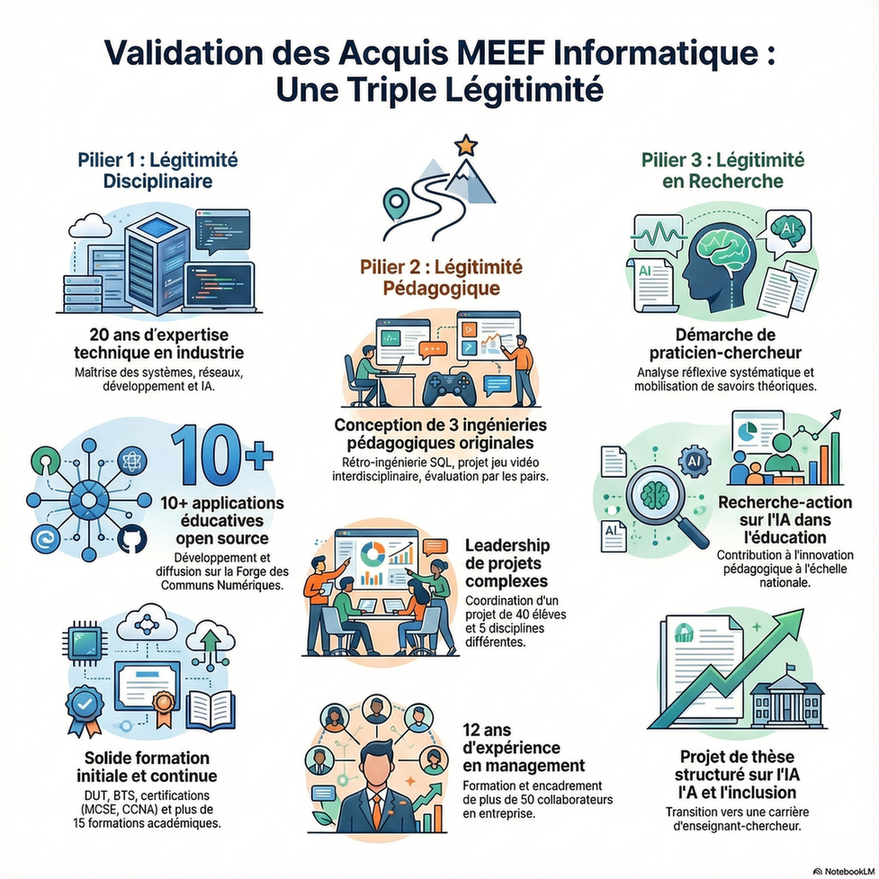
\includegraphics[width=0.8\textwidth]{sources/medias/p3-moy.png} \\ \vspace{0.5cm} \small \textit{Illustration réalisée avec NotebookLM}}
\chapter{Introduction : Méthodologie de correspondance}

Cette troisième partie établit les correspondances explicites entre mon parcours professionnel, les expériences détaillées en Partie 2, et le référentiel RNCP38152 du Master MEEF Pratiques et Ingénierie de la Formation (PIF) \parencite{rncp38152}. Elle démontre que mes acquis couvrent l'intégralité des 9 blocs de compétences attendus pour l'obtention du diplôme par validation des acquis de l'expérience \parencite{vademecum_vae_inspe}.

\section{Cadre de référence : le RNCP38152}

Le référentiel RNCP38152 « MASTER - Métiers de l'enseignement, de l'éducation et de la formation (MEEF), pratiques et ingénierie de la formation » définit les compétences attendues d'un expert en ingénierie de formation à un niveau de qualification 7 (Bac+5) \parencite{rncp38152,referentiel_meef}.

Ces compétences s'organisent en 9 blocs couvrant l'ensemble des dimensions de l'ingénierie de formation, de la conception à l'évaluation, en passant par le pilotage de projets et l'analyse réflexive \parencite{competences_transversales}.

\section{Méthodologie d'analyse}

Pour chaque bloc de compétences, je présenterai :

\begin{enumerate}[leftmargin=*]
    \item \textbf{La définition officielle} du bloc selon le référentiel RNCP38152
    \item \textbf{Les compétences détaillées} attendues
    \item \textbf{Mes expériences correspondantes} : références précises aux situations décrites dans la Partie 2 et mon parcours (Partie 1)
    \item \textbf{Les preuves tangibles} : productions, réalisations, attestations
    \item \textbf{Le niveau de maîtrise atteint} : indication du degré d'expertise développé
\end{enumerate}

Cette approche systématique permet au jury VAE d'évaluer objectivement l'adéquation entre mes acquis et les attendus du diplôme \parencite{vademecum_vae_inspe}.

\chapter{Analyse détaillée des 9 blocs de compétences RNCP38152}

Ce chapitre présente une analyse approfondie de la correspondance entre mon parcours professionnel et les 9 blocs de compétences du référentiel RNCP38152 du Master MEEF Pratiques et Ingénierie de la Formation (PIF).

\section{BC01 - Mettre en œuvre les usages avancés et spécialisés des outils numériques}

\subsection{Définition officielle du bloc}
\begin{quote}
\textit{« Identifier les usages numériques et les impacts de leur évolution sur le ou les domaines concernés par la mention. Se servir de façon autonome des outils numériques avancés pour un ou plusieurs métiers ou secteurs de recherche du domaine. »} \parencite{rncp38152}
\end{quote}

\subsection{Correspondance avec mon parcours}

\subsubsection{Expertise technique et ingénierie numérique}
Mon parcours de 20 ans dans l'industrie logicielle m'a permis de développer une expertise avancée des outils numériques, fondamentale pour l'ingénierie de formation moderne.
\begin{itemize}[leftmargin=*]
    \item \textbf{Maîtrise technologique} : Langages (Python, SQL, Web), architectures systèmes, et outils de versionning (Git/GitLab), essentiels pour concevoir des environnements d'apprentissage numériques (EIAH).
    \item \textbf{Création d'outils pour la formation} : Développement de la plateforme « Notation à l'Enveloppe » (Partie 2, Expérience 3) et du moteur de jeu éducatif (Partie 2, Expérience 2).
\end{itemize}

\subsubsection{Impact sur l'ingénierie de formation}
Je ne suis pas seulement utilisateur, mais concepteur d'outils numériques pour la formation.
\begin{itemize}[leftmargin=*]
    \item \textbf{Forge des Communs Numériques} : Contribution active au développement et partage de ressources éducatives libres (REL).
    \item \textbf{IA et Éducation} : Analyse critique et expérimentation des impacts de l'IA générative sur les pratiques de formation (Projet de thèse).
\end{itemize}

\textbf{Niveau de maîtrise : Expert} - Capacité démontrée à créer des outils numériques sur mesure pour des besoins de formation spécifiques.

\vspace{1cm}

\section{BC02 - Mobiliser et produire des savoirs hautement spécialisés}

\subsection{Définition officielle du bloc}
\begin{quote}
\textit{« Mobiliser des savoirs hautement spécialisés... Développer une conscience critique... Résoudre des problèmes... Conduire une analyse réflexive... »} \parencite{rncp38152}
\end{quote}

\subsection{Correspondance avec mon parcours}

\subsubsection{Savoirs disciplinaires et didactiques}
\begin{itemize}[leftmargin=*]
    \item \textbf{Double compétence} : Alliance de savoirs techniques pointus (NSI, développement) et de savoirs pédagogiques (didactique de l'informatique, ingénierie de formation).
    \item \textbf{Analyse de pratiques} : Utilisation de cadres théoriques (didactique professionnelle, approche par compétences) pour analyser les situations de formation (cf. Partie 2).
\end{itemize}

\subsubsection{Production de savoirs nouveaux}
\begin{itemize}[leftmargin=*]
    \item \textbf{Innovation méthodologique} : Conception de la méthode de « Notation à l'Enveloppe », une réponse originale à la problématique de l'évaluation des compétences transversales.
    \item \textbf{Recherche} : Engagement dans une démarche de recherche-action sur l'intégration de l'IA en didactique de l'informatique.
\end{itemize}

\textbf{Niveau de maîtrise : Avancé} - Capacité à articuler savoirs théoriques et savoirs d'action pour innover.

\vspace{1cm}

\section{BC03 - Mettre en œuvre une communication spécialisée pour le transfert de connaissances}

\subsection{Définition officielle du bloc}
\begin{quote}
\textit{« Identifier, sélectionner et analyser avec esprit critique diverses ressources spécialisées. Communiquer à des fins de formation ou de transfert de connaissances... »} \parencite{rncp38152}
\end{quote}

\subsection{Correspondance avec mon parcours}

\subsubsection{Communication pédagogique et formation d'adultes}
\begin{itemize}[leftmargin=*]
    \item \textbf{Formation de formateurs} : Animation d'ateliers et accompagnement de collègues sur les outils numériques et la pédagogie de projet.
    \item \textbf{Vulgarisation technique} : Capacité à rendre accessibles des concepts informatiques complexes (SQL, Algorithmique) à des publics variés (élèves, étudiants IUT, collègues).
\end{itemize}

\subsubsection{Médiation scientifique et technique}
\begin{itemize}[leftmargin=*]
    \item \textbf{Documentation et partage} : Rédaction de documentations techniques pédagogiques sur la Forge et le site \textit{home.educ-ai.fr}.
    \item \textbf{Rayonnement} : Communication professionnelle lors de groupes de travail académiques.
\end{itemize}

\textbf{Niveau de maîtrise : Avancé} - Expertise dans la transmission de savoirs techniques et méthodologiques.

\vspace{1cm}

\section{BC04 - Contribuer à la transformation en contexte professionnel}

\subsection{Définition officielle du bloc}
\begin{quote}
\textit{« Gérer des contextes professionnels complexes... Conduire un projet... Analyser ses actions... Respecter les principes d'éthique... »} \parencite{rncp38152}
\end{quote}

\subsection{Correspondance avec mon parcours}

\subsubsection{Pilotage de projets complexes}
\begin{itemize}[leftmargin=*]
    \item \textbf{Gestion de projet industriel} : 12 ans d'expérience en tant que Team Leader, gestion de budgets et d'équipes, transférable à la gestion de projets de formation.
    \item \textbf{Projets interdisciplinaires} : Pilotage du projet « Jeu Vidéo » (Partie 2), coordonnant 5 enseignants et 40 élèves sur 8 mois.
\end{itemize}

\subsubsection{Démarche qualité et éthique}
\begin{itemize}[leftmargin=*]
    \item \textbf{Amélioration continue} : Application des méthodes agiles (Scrum, feedback) à l'ingénierie de formation.
    \item \textbf{Éthique du numérique} : Intégration systématique des enjeux RGPD, accessibilité (W3C) et inclusion dans les projets numériques développés.
\end{itemize}

\textbf{Niveau de maîtrise : Expert} - Compétences éprouvées en gestion de projet et accompagnement du changement.

\vspace{1cm}

\section{BC05 - Concevoir, piloter et animer des dispositifs ou ingénieries de formation ou de médiation}

\subsection{Définition officielle du bloc}
\begin{quote}
\textit{« Recueillir des besoins, formaliser un projet de formation. Établir et mettre en œuvre un cahier des charges. Mobiliser des savoirs spécialisés... »} \parencite{rncp38152}
\end{quote}

\subsection{Correspondance avec mon parcours}

\subsubsection{Ingénierie didactique et pédagogique}
\begin{itemize}[leftmargin=*]
    \item \textbf{Analyse des besoins} : Diagnostic des difficultés d'apprentissage du SQL (Partie 2) pour concevoir un dispositif de remédiation par rétro-ingénierie.
    \item \textbf{Conception de dispositifs} : Création de scénarios pédagogiques complets (progressions, séquences, évaluations) adaptés aux publics (Lycée, IUT).
\end{itemize}

\subsubsection{Adaptation aux publics}
\begin{itemize}[leftmargin=*]
    \item \textbf{Différenciation} : Conception de parcours adaptés aux élèves à besoins particuliers (ULIS, troubles dys) grâce au numérique.
    \item \textbf{Publics hétérogènes} : Adaptation des stratégies pédagogiques pour des groupes variés (scientifiques, tertiaires).
\end{itemize}

\textbf{Niveau de maîtrise : Avancé} - Capacité à concevoir des ingénieries complètes, de l'analyse des besoins à l'évaluation.

\vspace{1cm}

\section{BC06 - Situer ses interventions dans un écosystème professionnel, coopérer, co-construire des actions}

\subsection{Définition officielle du bloc}
\begin{quote}
\textit{« Inscrire son action dans un secteur professionnel de formation... Conduire un projet dans un cadre collaboratif... Contribuer à la performance stratégique d'une équipe. »} \parencite{rncp38152}
\end{quote}

\subsection{Correspondance avec mon parcours}

\subsubsection{Travail collaboratif et réseau}
\begin{itemize}[leftmargin=*]
    \item \textbf{Co-construction} : Travail en équipe pluridisciplinaire (Lettres, Arts, Langues, Info) pour le projet Jeu Vidéo.
    \item \textbf{Réseaux professionnels} : Participation active aux réseaux d'enseignants NSI et à la communauté de la Forge des Communs Numériques.
\end{itemize}

\subsubsection{Partenariats}
\begin{itemize}[leftmargin=*]
    \item \textbf{Lien École-Entreprise} : Mobilisation de mon réseau professionnel pour l'orientation des élèves et l'intervention d'experts.
    \item \textbf{Écosystème numérique} : Collaboration avec les acteurs du numérique éducatif (DNE, académie).
\end{itemize}

\textbf{Niveau de maîtrise : Acquis} - Forte culture de la coopération issue du monde de l'entreprise et réinvestie dans l'éducation.

\vspace{1cm}

\section{BC07 - Produire et diffuser des ressources, des outils, des démarches, et des contenus de formation innovants}

\subsection{Définition officielle du bloc}
\begin{quote}
\textit{« Identifier des besoins en termes de ressources. Adapter la production... Faire évoluer les modalités d'enseignement... Identifier le processus de production, de diffusion et de valorisation des savoirs. »} \parencite{rncp38152}
\end{quote}

\subsection{Correspondance avec mon parcours}

\subsubsection{Conception de ressources innovantes}
\begin{itemize}[leftmargin=*]
    \item \textbf{Outils numériques} : Développement d'applications web pour l'apprentissage (Quiz, IDE en ligne, outils de gestion de projet).
    \item \textbf{Supports pédagogiques} : Création de capsules vidéo, de tutoriels interactifs et de supports de cours différenciés.
\end{itemize}

\subsubsection{Diffusion et valorisation}
\begin{itemize}[leftmargin=*]
    \item \textbf{Open Source} : Publication des outils développés sous licences libres pour favoriser leur réutilisation par la communauté éducative.
    \item \textbf{Partage d'expertise} : Diffusion de pratiques innovantes (méthode d'évaluation, pédagogie de projet) auprès des pairs.
\end{itemize}

\textbf{Niveau de maîtrise : Expert} - Production significative de ressources numériques utilisées par d'autres formateurs.

\vspace{1cm}

\section{BC08 - Conduire, piloter et partager une analyse réflexive sur les pratiques}

\subsection{Définition officielle du bloc}
\begin{quote}
\textit{« Accompagner des professionnels en formation dans l'analyse de leurs pratiques... Former les formateurs à prendre en compte les critiques et à réajuster les pratiques. »} \parencite{rncp38152}
\end{quote}

\subsection{Correspondance avec mon parcours}

\subsubsection{Analyse de pratiques}
\begin{itemize}[leftmargin=*]
    \item \textbf{Auto-analyse} : Pratique réflexive systématique sur mes propres enseignements (cf. bilans d'expériences Partie 2).
    \item \textbf{Accompagnement} : Rôle de tuteur informel auprès de collègues débutants en NSI, aide à l'analyse de leurs difficultés techniques et pédagogiques.
\end{itemize}

\subsubsection{Démarche qualité}
\begin{itemize}[leftmargin=*]
    \item \textbf{Évaluation des dispositifs} : Mise en place d'indicateurs pour mesurer l'efficacité des formations et des outils (réussite aux examens, satisfaction, engagement).
    \item \textbf{Régulation} : Ajustement continu des scénarios pédagogiques basé sur l'analyse des résultats et les retours des apprenants.
\end{itemize}

\textbf{Niveau de maîtrise : Avancé} - Posture réflexive ancrée et capacité à accompagner l'analyse de pratiques.

\vspace{1cm}

\section{BC09 - S'engager dans une démarche de développement professionnel}

\subsection{Définition officielle du bloc}
\begin{quote}
\textit{« Se tenir informé des évolutions de la recherche scientifique... Conduire une analyse réflexive... Développer des ingénieries pédagogiques et didactiques dans une perspective d'enseignement, de formation, de recherche. »} \parencite{rncp38152}
\end{quote}

\subsection{Correspondance avec mon parcours}

\subsubsection{Développement professionnel continu}
\begin{itemize}[leftmargin=*]
    \item \textbf{Formation continue} : Suivi de nombreuses formations académiques et auto-formation technique permanente.
    \item \textbf{Recherche} : Engagement dans un projet de thèse, lecture de la littérature scientifique en didactique et sciences de l'éducation.
\end{itemize}

\subsubsection{Perspective de recherche}
\begin{itemize}[leftmargin=*]
    \item \textbf{Ingénierie didactique} : Conception de situations d'apprentissage fondées sur la recherche (problématisation, institutionnalisation).
    \item \textbf{Veille} : Suivi actif des innovations en technologies éducatives (IA, Learning Analytics).
\end{itemize}

\textbf{Niveau de maîtrise : Acquis} - Engagement fort dans une dynamique de chercheur-praticien.

\chapter{Contribution des expériences à la maîtrise des compétences}

\section{Tableau croisé Expériences $\leftrightarrow$ Blocs RNCP38152}

Les trois expériences pédagogiques analysées en Partie 2 illustrent de manière concrète ma maîtrise des compétences du référentiel RNCP38152. Le tableau suivant présente leur contribution spécifique aux 9 blocs de compétences :

\begin{table}[htbp]
\centering
\begin{tabular}{|l|c|c|c|}
\hline
\textbf{Bloc RNCP} & \textbf{FORGÉALES} & \textbf{JEUX} & \textbf{ÉVAL} \\
\hline
\textbf{BC01} & ++ & +++ & ++ \\
\hline
\textbf{BC02} & +++ & ++ & ++ \\
\hline
\textbf{BC03} & ++ & +++ & ++ \\
\hline
\textbf{BC04} & - & +++ & ++ \\
\hline
\textbf{BC05} & +++ & +++ & +++ \\
\hline
\textbf{BC06} & +++ & +++ & +++ \\
\hline
\textbf{BC07} & - & ++ & ++ \\
\hline
\textbf{BC08} & ++ & +++ & ++ \\
\hline
\textbf{BC09} & ++ & +++ & ++ \\
\hline
\end{tabular}
\caption{Tableau croisé : Contribution des expériences aux blocs RNCP38152}
\end{table}

\subsection{Légende des niveaux de contribution}

\begin{itemize}[leftmargin=*]
    \item \textbf{+++} : \textbf{Contribution majeure} - L'expérience démontre une maîtrise approfondie du bloc.
    \item \textbf{++} : \textbf{Contribution significative} - L'expérience apporte des preuves tangibles de compétence.
    \item \textbf{-} : Contribution indirecte ou non applicable.
\end{itemize}

\subsection{Analyse des contributions}

\subsubsection{Expérience FORGÉALES - Formation de formateurs à l'IA et \LaTeX{}}

\textbf{Points forts} :
\begin{itemize}[leftmargin=*]
    \item \textbf{BC01/BC03/BC07} : Conception et diffusion d'une formation numérique de formateurs avec production de ressources libres sur la Forge.
    \item \textbf{BC05/BC06} : Ingénierie de formation d'adultes (andragogie) et animation d'ateliers synchrones/asynchrones.
    \item Maîtrise des technologies émergentes (IA générative) pour l'écriture scientifique structurée.
    \item Accompagnement individualisé et collectif des enseignants et formateurs.
\end{itemize}

\subsubsection{Expérience JEUX - Pilotage de projet complexe}

\textbf{Couverture étendue des blocs} :
\begin{itemize}[leftmargin=*]
    \item \textbf{BC04/BC06} : Pilotage d'un projet complexe et collaboratif (5 disciplines, 40+ apprenants).
    \item \textbf{BC01/BC07} : Développement d'un moteur de jeu complet (outil numérique sur mesure) et diffusion sur la Forge.
    \item \textbf{BC05} : Conception et animation d'un dispositif de formation par projet.
    \item \textbf{BC03} : Communication et valorisation du projet auprès de la communauté.
\end{itemize}

\subsubsection{Expérience ÉVALUATION - Innovation en évaluation}

\textbf{Spécialisation en évaluation et métacognition} :
\begin{itemize}[leftmargin=*]
    \item \textbf{BC05/BC07} : Création d'un outil d'évaluation innovant ("Notation à l'Enveloppe").
    \item Développement de l'auto-évaluation et de la pratique réflexive chez les apprenants (BC08).
    \item Différenciation pédagogique et adaptation aux profils d'apprentissage.
    \item Modélisation d'une grille d'évaluation transférable (Ingénierie).
\end{itemize}

\section{Transfert des expériences vers l'enseignement supérieur}

\subsection{Adaptation des innovations à l'IUT}

Mon arrivée en IUT en 2025 m'a permis de commencer à transférer les approches pédagogiques développées en lycée.

\subsubsection{Adaptation de la méthode SQL}

\textbf{Contexte} : Étudiants de BUT Techniques de Commercialisation avec des niveaux hétérogènes.
\begin{itemize}[leftmargin=*]
    \item Application de la rétro-ingénierie aux systèmes d'information commerciaux.
    \item Création du besoin par l'analyse de cas concrets d'entreprises partenaires.
    \item Progression du terrain professionnel vers les concepts techniques.
\end{itemize}

\subsubsection{Projet interdisciplinaire à l'IUT}

\textbf{Projet en cours} : Projet transversal entre les départements BUT TC et Informatique.
\begin{itemize}[leftmargin=*]
    \item Développement d'applications mobiles de gestion commerciale.
    \item Collaboration entre étudiants TC (expression du besoin métier) et informatique (réalisation de la solution technique).
    \item Adaptation des méthodes agiles au rythme universitaire.
\end{itemize}

\subsubsection{Évaluation par les pairs dans le supérieur}

\textbf{Expérimentation prévue en 2025-2026} :
\begin{itemize}[leftmargin=*]
    \item Mise en place d'une évaluation croisée des projets entre groupes d'étudiants.
    \item Développement de l'esprit critique et de l'auto-évaluation.
    \item Préparation aux soutenances et à la communication professionnelle.
\end{itemize}

\subsection{Contribution à l'innovation pédagogique}

\subsubsection{Hub de ressources numériques}

\textbf{Développement en cours} :
\begin{itemize}[leftmargin=*]
    \item Adaptation des applications de la Forge aux spécificités de l'IUT.
    \item Formation de collègues aux outils numériques.
    \item Création d'une communauté de pratiques au sein du département.
\end{itemize}

\subsubsection{Recherche-action sur l'IA}

\textbf{Extension du projet de thèse} :
\begin{itemize}[leftmargin=*]
    \item Expérimentation de l'IA générative pour la personnalisation des apprentissages.
    \item Analyse de l'impact sur les étudiants à besoins particuliers en contexte universitaire.
    \item Documentation en vue d'une diffusion dans d'autres IUT.
\end{itemize}

\subsection{Rayonnement et partage}

\subsubsection{Formation des pairs}

\textbf{Actions menées et prévues} :
\begin{itemize}[leftmargin=*]
    \item Sessions de formation aux outils de la Forge des Communs.
    \item Ateliers sur la pédagogie de projet adaptée au supérieur.
    \item Partage méthodologique inter-départements.
\end{itemize}

\subsubsection{Publications et communications}

\textbf{Valorisation scientifique envisagée} :
\begin{itemize}[leftmargin=*]
    \item Rédaction d'un article sur la transposition des innovations pédagogiques du lycée à l'IUT.
    \item Proposition de communication au colloque QPES (Questions de Pédagogie dans l'Enseignement Supérieur).
    \item Contribution aux journées nationales des IUT informatique.
\end{itemize}

\chapter{Synthèse de la correspondance}

\section{Tableau récapitulatif de couverture des blocs de compétences RNCP38152}

\begin{landscape}

\begin{longtable}{|p{4cm}|p{9cm}|p{11cm}|}
\caption{Synthèse de la correspondance parcours - RNCP38152} \\
\hline
\textbf{Bloc RNCP} & \textbf{Expériences principales} & \textbf{Preuves tangibles} \\
\hline
\endfirsthead
\hline
\textbf{Bloc RNCP} & \textbf{Expériences principales} & \textbf{Preuves tangibles} \\
\hline
\endhead
\hline
\endfoot

\textbf{BC01 - Usages numériques} &
20 ans d'expertise technique, développement d'EIAH, conception d'outils sur mesure (moteur de jeu, outil d'évaluation) &
Applications sur la Forge, Code source du moteur de jeu, Plateforme "Notation à l'Enveloppe" \\
\hline

\textbf{BC02 - Savoirs spécialisés} &
Double compétence expert technique / ingénieur pédagogique, innovation méthodologique &
Diplômes techniques, méthode "Notation à l'Enveloppe", productions didactiques \\
\hline

\textbf{BC03 - Communication} &
Formation de formateurs, documentation technique et pédagogique, vulgarisation &
Supports de formation, documentation Forge, site web éducatif \\
\hline

\textbf{BC04 - Transformation pro} &
Pilotage de projets complexes (industrie \& éducation), gestion d'équipes pluridisciplinaires &
Projet Jeu Vidéo (5 enseignants, 40 élèves), management d'équipes techniques (12 ans) \\
\hline

\textbf{BC05 - Ingénierie formation} &
Conception de dispositifs complets (SQL, Jeu), analyse des besoins, scénarisation &
Scénarios pédagogiques, grilles d'évaluation, plans de formation \\
\hline

\textbf{BC06 - Écosystème \& Coopération} &
Travail collaboratif en réseau (Forge, NSI), projets interdisciplinaires &
Contributions open source, projet inter-matières, partenariats académiques \\
\hline

\textbf{BC07 - Production ressources} &
Création et diffusion de ressources numériques innovantes (REL), outils d'évaluation &
10+ applications libres, tutoriels vidéo, fiches pédagogiques \\
\hline

\textbf{BC08 - Analyse réflexive} &
Accompagnement de pairs, auto-analyse systématique des dispositifs, démarche qualité &
Bilans d'expériences (Partie 2), ajustements des scénarios, mentorat informel \\
\hline

\textbf{BC09 - Développement pro} &
Veille scientifique (IA, didactique), formation continue, recherche-action &
Projet de thèse, bibliographie, participation à des groupes de travail \\
\hline

\end{longtable}

\end{landscape}

\section{Conclusion : Une expertise en ingénierie de formation}

L'analyse de la correspondance entre mon parcours et le référentiel RNCP38152 met en évidence une couverture étendue des 9 blocs de compétences attendus pour le Master MEEF PIF. Cette adéquation repose sur trois piliers complémentaires :

\subsection{Expertise technologique au service de la formation}

\begin{itemize}[leftmargin=*]
    \item 20 ans d'expérience technique de haut niveau réinvestis dans la conception d'outils pour la formation (BC01, BC07).
    \item Une capacité à anticiper les évolutions numériques (IA) pour adapter les ingénieries de formation.
\end{itemize}

\subsection{Compétences en ingénierie pédagogique}

\begin{itemize}[leftmargin=*]
    \item Conception et pilotage de dispositifs de formation complexes et innovants (BC04, BC05).
    \item Une approche systémique de la formation, intégrant l'analyse des besoins, la conception, l'animation et l'évaluation.
\end{itemize}

\subsection{Posture de praticien-chercheur et formateur de formateurs}

\begin{itemize}[leftmargin=*]
    \item Une démarche réflexive constante et partagée (BC08, BC09).
    \item Une contribution active à la communauté éducative par la production de savoirs et de ressources (BC02, BC06).
\end{itemize}

\vspace{1cm}

Cette triple légitimité constitue un socle solide pour valider le Master MEEF PIF et poursuivre vers une carrière d'ingénieur de formation ou d'enseignant-chercheur.

\chapter{Projet professionnel et perspectives de recherche}

\section{Projet de thèse : \enquote{Conception et Évaluation d'un Écosystème d'IA Co-adaptatif pour l'Inclusion Pédagogique Active}}

\subsection{Cadre et problématique}

Ce projet de thèse, envisagé au sein du laboratoire LITIS (UR 4108) sous la direction du Professeur Laurent Heutte et en collaboration avec Élisabeth SCHNEIDER (CIRNEF / ESO UMR 6590, Unicaen), vise à répondre à une problématique centrale de l'école inclusive : comment l'Intelligence Artificielle peut-elle devenir un partenaire co-adaptatif pour le triptyque élève-AESH-enseignant ?

L'objectif est de concevoir un écosystème socio-technique capable d'automatiser l'adaptation de contenus pédagogiques tout en maintenant une boucle de rétroaction humaine (Human-in-the-loop). Ce projet se situe à la confluence de trois domaines :
\begin{itemize}
    \item \textbf{Document Intelligence (IA)} : Pour l'analyse sémantique profonde des supports pédagogiques.
    \item \textbf{Interaction Homme-Machine (IHM)} : Pour garantir l'explicabilité et l'appropriation de l'outil par les enseignants (genèse instrumentale).
    \item \textbf{Apprentissage par Renforcement (RLHF)} : Pour aligner le système sur les objectifs pédagogiques réels via les retours des utilisateurs.
\end{itemize}

\subsection{Méthodologie et calendrier prévisionnel (2026-2029)}

La recherche se structurera en trois phases sur 3 ans :
\begin{enumerate}
    \item \textbf{Année 1 : Co-conception.} Immersion ethnographique et ateliers avec les utilisateurs (enseignants, AESH, élèves) pour modéliser les besoins et définir le cahier des charges.
    \item \textbf{Année 2 : Prototypage.} Développement d'un prototype open-source intégrant des modules d'adaptation multimodale (simplification de texte, description d'images, reformatage).
    \item \textbf{Année 3 : Expérimentation.} Déploiement en conditions réelles (IUT, lycée) et évaluation de l'impact sur l'autonomie des élèves et la charge de travail des accompagnants.
\end{enumerate}

Ce travail vise des contributions scientifiques (modélisation de l'IA co-adaptative), technologiques (outils open-source) et sociales (amélioration de l'inclusion).

\section{Trajectoire professionnelle et cohérence du projet VAE}

\subsection{Plan de carrière}

L'obtention du Master MEEF par VAE est la clé de voûte de ma transition professionnelle :
\begin{itemize}
    \item \textbf{Court terme (2025-2026)} : Consolidation de mon poste de PRCE à l'IUT du Havre et préparation de l'entrée en thèse.
    \item \textbf{Moyen terme (2026-2029)} : Réalisation du doctorat tout en poursuivant l'innovation pédagogique (Forge des Communs).
    \item \textbf{Long terme} : Qualification aux fonctions de Maître de Conférences pour diriger des recherches sur l'IA éducative.
\end{itemize}

\subsection{Le Master MEEF : un levier stratégique}

Ce diplôme ne constitue pas seulement une validation des acquis, mais un véritable tremplin. Il légitime 25 ans d'expérience technique et pédagogique, transformant un parcours atypique en une expertise académique reconnue. Il assure la continuité entre mon passé industriel, mon présent d'enseignant et mon futur de chercheur, avec pour fil rouge constant l'innovation au service de l'inclusion.


% ===========================
% CONCLUSION GÉNÉRALE
% ===========================

\chapter*{Conclusion générale}
\addcontentsline{toc}{chapter}{Conclusion générale}

Cette démarche de Validation des Acquis de l'Expérience s'inscrit dans le prolongement d'une trajectoire professionnelle continue dans l'éducation et la formation. À travers l'analyse de mon parcours et des trois expériences présentées, ce dossier vise à démontrer la correspondance de mes acquis avec les exigences du Master MEEF PIF (Pratiques et Ingénierie de la Formation) tel que défini par le référentiel RNCP38152 \parencite{rncp38152}.

\section*{Un parcours professionnel transformé en expertise pédagogique}

\subsection*{De l'industrie vers l'éducation : une reconversion maîtrisée}

Mon parcours professionnel de 25 années illustre une évolution remarquable : celle d'un expert technique industriel devenu praticien-chercheur en éducation. Cette transformation ne s'est pas opérée par accident, mais résulte d'une réflexion profonde sur le sens de l'engagement professionnel et la volonté de contribuer à la formation des générations futures dans un domaine en perpétuelle mutation \parencite{perrenoud_pratique_reflexive}.

Les 20 années d'expérience en développement logiciel, administration de systèmes complexes et management d'équipes techniques constituent bien plus qu'un simple bagage technique. Elles représentent une compréhension intime des enjeux du numérique contemporain, une capacité éprouvée à résoudre des problèmes complexes et une vision stratégique des évolutions technologiques. Cette expertise, enrichie par une formation continue constante et des certifications professionnelles, couvre les domaines de l'ingénierie et de la didactique de la formation du Master MEEF PIF.

\subsection*{Une philosophie pédagogique innovante et cohérente}

L'analyse des trois expériences professionnelles révèle l'émergence d'une philosophie pédagogique personnelle, structurée autour de principes forts :

\begin{itemize}[leftmargin=*]
    \item \textbf{L'apprentissage par investigation} : Placer l'apprenant en position d'enquêteur face à des problématiques authentiques
    \item \textbf{La collaboration interdisciplinaire} : Décloisonner les apprentissages pour révéler la richesse des interactions entre domaines
    \item \textbf{L'évaluation équitable et formative} : Transformer l'évaluation en levier d'apprentissage et de développement de l'autonomie
    \item \textbf{L'innovation méthodologique} : Créer de nouveaux outils pédagogiques pour répondre aux défis contemporains de l'éducation
\end{itemize}

Cette approche pédagogique ne relève pas de l'application mécanique de recettes, mais témoigne d'une réflexion approfondie sur les finalités éducatives et les moyens de les atteindre. Elle s'appuie sur une solide culture théorique en sciences de l'éducation et se nourrit d'une pratique réflexive constante \parencite{schon_reflective_practitioner}.

\section*{Une contribution unique à la communauté éducative}

\subsection*{Expertise technique au service de l'innovation pédagogique}

Mon profil présente une particularité intéressante dans le paysage de l'enseignement de l'informatique : la combinaison d'une expérience technique industrielle substantielle avec des compétences en ingénierie pédagogique. Cette double expérience me permet de mieux comprendre les besoins de formation, de concevoir des dispositifs pédagogiques en lien avec les évolutions technologiques et de préparer les étudiants aux réalités professionnelles qu'ils rencontreront.

La création du moteur de jeu éducatif, la conception de la méthode de "Notation à l'Enveloppe" ou le développement de supports pédagogiques innovants illustrent cette capacité à mobiliser l'expertise technique au service de l'apprentissage. Ces réalisations témoignent d'un engagement dans l'innovation pédagogique et constituent des éléments significatifs de cette candidature VAE.

\subsection*{Leadership pédagogique et rayonnement institutionnel}

Les expériences présentées révèlent une capacité à fédérer, animer et coordonner des équipes pédagogiques pluridisciplinaires. Le projet de jeu vidéo interdisciplinaire, impliquant 5 enseignants et 40 élèves, témoigne de compétences en animation d'équipe qui s'étendent au-delà du cadre habituel de la classe. Cette aptitude à créer et animer une dynamique collective constitue un atout pour l'évolution vers l'enseignement supérieur et la recherche.

Le rayonnement de ces actions au-delà de l'établissement d'origine, leur reconnaissance institutionnelle et leur documentation rigoureuse en vue d'une diffusion plus large illustrent une posture de praticien-chercheur déjà mature. Cette dimension de recherche-action, essentielle dans la formation des enseignants, est ici pleinement développée \parencite{recherche_action_education}.

\section*{Perspectives d'évolution et projet professionnel}

\subsection*{Vision stratégique de l'enseignement supérieur}

L'obtention du Master MEEF PIF par VAE s'inscrit dans une démarche professionnelle réfléchie et structurée. Mon affectation actuelle en BUT Techniques de Commercialisation à l'IUT du Havre me permet d'expérimenter progressivement le transfert de mes compétences vers l'enseignement supérieur, même si ce n'est pas directement dans ma discipline de formation.

L'enseignement en IUT présente des spécificités qui résonnent avec les expériences que j'ai développées : public hétérogène nécessitant une adaptation pédagogique, formation professionnalisante valorisant l'expérience du monde de l'entreprise, pédagogie de projet intégrée aux cursus. Ces caractéristiques me permettent d'appliquer progressivement les approches pédagogiques expérimentées dans l'enseignement secondaire.

\subsection*{Contribution à la recherche en éducation}

Mon projet de thèse sur l'impact pédagogique de l'intelligence artificielle dans l'enseignement de l'informatique s'enracine directement dans les questionnements soulevés par ma pratique professionnelle. Cette recherche ne constitue pas une fuite vers l'abstraction théorique, mais l'approfondissement scientifique de problématiques concrètes rencontrées sur le terrain.

Les perspectives de recherche identifiées dans chaque expérience (personnalisation automatique des supports pédagogiques, évaluation objective des compétences transversales, optimisation de la collaboration interdisciplinaire numérique) convergent vers des enjeux majeurs de l'éducation contemporaine \parencite{intelligence_artificielle_education}. Cette cohérence entre pratique professionnelle et projet de recherche témoigne d'une maturité scientifique rare chez un candidat VAE.

\section*{Engagement dans la profession : vision et responsabilités}

\subsection*{Responsabilité éthique et sociale}

Mon engagement dans la profession enseignante dépasse largement la transmission de savoirs techniques. Il s'ancre dans une conviction profonde : celle de la responsabilité éthique et sociale de tout éducateur face aux défis du XXIe siècle. Dans un monde où l'intelligence artificielle transforme radicalement les métiers du numérique, où les enjeux de cybersécurité deviennent critiques, où les questions d'éthique numérique se posent avec acuité, l'enseignant d'informatique porte une responsabilité particulière.

Je m'engage à former non seulement des techniciens compétents, mais des citoyens numériques éclairés, capables de comprendre les enjeux de leur domaine d'expertise et d'agir de manière responsable. Cette dimension citoyenne de l'enseignement de l'informatique constitue l'un des fils rouges de mon projet professionnel \parencite{competences_21_siecle}.

\subsection*{Innovation pédagogique et transformation numérique de l'éducation}

L'évolution rapide des technologies numériques impose aux enseignants d'informatique une responsabilité particulière dans l'innovation pédagogique. Fort de mon expertise technique et de ma capacité démontrée d'innovation méthodologique, je m'engage à contribuer activement à la transformation numérique de l'éducation.

Cette contribution s'articulera autour de trois axes stratégiques :

\subsubsection*{Développement d'outils pédagogiques innovants}

La création de nouveaux outils numériques au service de l'apprentissage, à l'image du moteur de jeu éducatif développé ou de la plateforme d'évaluation par les pairs envisagée. Ces outils, conçus avec une expertise technique de haut niveau et une connaissance fine des besoins pédagogiques, contribueront au patrimoine commun des ressources éducatives libres.

\subsubsection*{Formation des enseignants aux technologies émergentes}

L'accompagnement de mes collègues dans l'appropriation des nouvelles technologies éducatives, particulièrement l'intelligence artificielle. Cette mission de formation des formateurs s'appuie sur ma double expertise technique et pédagogique pour démystifier les technologies complexes et favoriser leur intégration raisonnée dans les pratiques d'enseignement.

\subsubsection*{Recherche appliquée en technologie éducative}

La conduite de recherches appliquées sur l'efficacité pédagogique des technologies numériques, en particulier l'intelligence artificielle. Ces recherches, ancrées dans la pratique de terrain, viseront à produire des connaissances scientifiquement validées et directement transférables dans les pratiques professionnelles.

\subsection*{Engagement institutionnel et rayonnement professionnel}

Mon engagement dans la profession se manifeste également par une participation active à la vie institutionnelle et au rayonnement de la discipline. Cette participation s'articule autour de plusieurs dimensions :

\subsubsection*{Contribution aux instances professionnelles}

Participation active aux groupes de travail institutionnels sur l'évolution des programmes d'informatique, l'intégration de l'intelligence artificielle dans l'enseignement, la définition des compétences numériques du XXIe siècle. Cette contribution s'appuie sur mon expérience de terrain et ma connaissance des enjeux industriels pour éclairer les décisions stratégiques.

\subsubsection*{Diffusion des pratiques innovantes}

Valorisation et diffusion des innovations pédagogiques développées à travers publications scientifiques, communications en colloques, formations d'enseignants. Cette démarche de partage s'inscrit dans une logique de contribution au bien commun éducatif et de développement collectif des pratiques professionnelles.

\subsubsection*{Dialogue avec le monde économique}

Maintien et développement de liens étroits avec le monde de l'entreprise pour assurer l'adéquation entre formation et besoins professionnels. Cette interface, facilitée par mon expérience industrielle, permettra d'anticiper les évolutions des métiers et d'adapter en conséquence les contenus et méthodes de formation.

\subsection*{Formation de la relève et transmission de l'expertise}

L'un des aspects les plus significatifs de mon engagement professionnel réside dans la formation de la nouvelle génération d'enseignants d'informatique. Mon parcours atypique et les compétences développées me positionnent naturellement comme ressource pour l'accompagnement des enseignants débutants.

Cette mission de formation de formateurs s'exercera à travers :

\begin{itemize}[leftmargin=*]
    \item \textbf{Tutorat des enseignants stagiaires} : Accompagnement personnalisé des nouveaux enseignants dans la construction de leur identité professionnelle
    \item \textbf{Formation continue} : Animation de stages de formation sur l'innovation pédagogique en informatique
    \item \textbf{Recherche collaborative} : Encadrement de travaux de recherche sur les pratiques d'enseignement en informatique
    \item \textbf{Production de ressources} : Élaboration de guides méthodologiques et d'outils d'aide à l'enseignement
\end{itemize}

\section*{Conclusion prospective : vers une carrière d'enseignant-chercheur}

Ce dossier de VAE marque une étape décisive dans ma trajectoire professionnelle, mais constitue également le point de départ d'un projet ambitieux : devenir un acteur reconnu de l'innovation pédagogique en informatique et contribuer significativement à l'évolution des pratiques d'enseignement dans ce domaine stratégique.

\subsection*{Synthèse du parcours}

L'analyse de mon parcours met en évidence une correspondance étroite avec les attendus du Master MEEF Pratiques et Ingénierie de la Formation. Les compétences développées, l'expérience du terrain et le projet de recherche s'inscrivent dans la continuité de cette démarche de validation des acquis.

Ce dossier vise à présenter la transférabilité de mes acquis professionnels vers l'ingénierie de formation et la recherche, en s'appuyant sur une expérience industrielle solide et une pratique réflexive engagée.

\subsection*{Positionnement pour l'avenir}

L'obtention du Master MEEF PIF par VAE me permettra de concrétiser pleinement mon projet professionnel d'enseignant-chercheur. Cette reconnaissance institutionnelle de mes compétences ouvrira la voie à :

\begin{itemize}[leftmargin=*]
    \item Une thèse de doctorat sur l'impact pédagogique de l'intelligence artificielle
    \item Une contribution significative à la recherche en technologie éducative
    \item Un rayonnement national et international dans le domaine de l'innovation pédagogique
    \item Une carrière d'enseignant-chercheur au service de la formation des futurs professionnels du numérique
\end{itemize}

\subsection*{Engagement pour l'avenir de l'éducation}

Au-delà de ma trajectoire personnelle, cet engagement s'inscrit dans une réflexion approfondie sur les enjeux contemporains de l'enseignement de l'informatique. La transformation numérique et l'essor de l'intelligence artificielle nécessitent une adaptation constante des pratiques pédagogiques pour former non seulement des techniciens compétents, mais surtout des citoyens éclairés et responsables.

Je souhaite mettre mon expertise technique et mes compétences pédagogiques au service d'une vision humaniste du numérique. Il s'agit de transmettre aux futurs professionnels les clés de compréhension d'un monde complexe, en alliant maîtrise technologique et conscience éthique. Cette démarche vise à favoriser l'émancipation intellectuelle des étudiants face aux outils qu'ils seront amenés à concevoir et à utiliser.

\vspace{1cm}

\begin{center}
\textit{\textbf{« L'objectif principal de l'éducation à l'école doit être de créer des hommes et des femmes qui sont capables de faire des choses nouvelles, non pas simplement de répéter ce que les autres générations ont fait. »}} \\
\vspace{0.2cm}
\textbf{Jean Piaget}
\end{center}

\vspace{0.5cm}

C'est dans cet esprit que j'envisage la suite de mon parcours d'enseignant, de formateur d'adultes et de futur enseignant-chercheur : guider les \textbf{élèves} du secondaire vers l'émancipation numérique et l'esprit critique, accompagner les \textbf{étudiants} du supérieur dans l'acquisition d'une haute maîtrise professionnelle par l'approche par compétences, et outiller les \textbf{formateurs et pairs enseignants} pour co-construire les pratiques pédagogiques de demain. Ma démarche VAE n'est ainsi pas une fin en soi, mais le point de départ d'un engagement renouvelé au service de l'accompagnement de tous les publics, de la transmission et de l'innovation pédagogique.

\newpage
\pagenumbering{gobble}

% ===========================
% INCLUSION DES ANNEXES
% ===========================
\part[Annexes Illustratives]{Annexes Illustratives \\ \vspace{2cm} 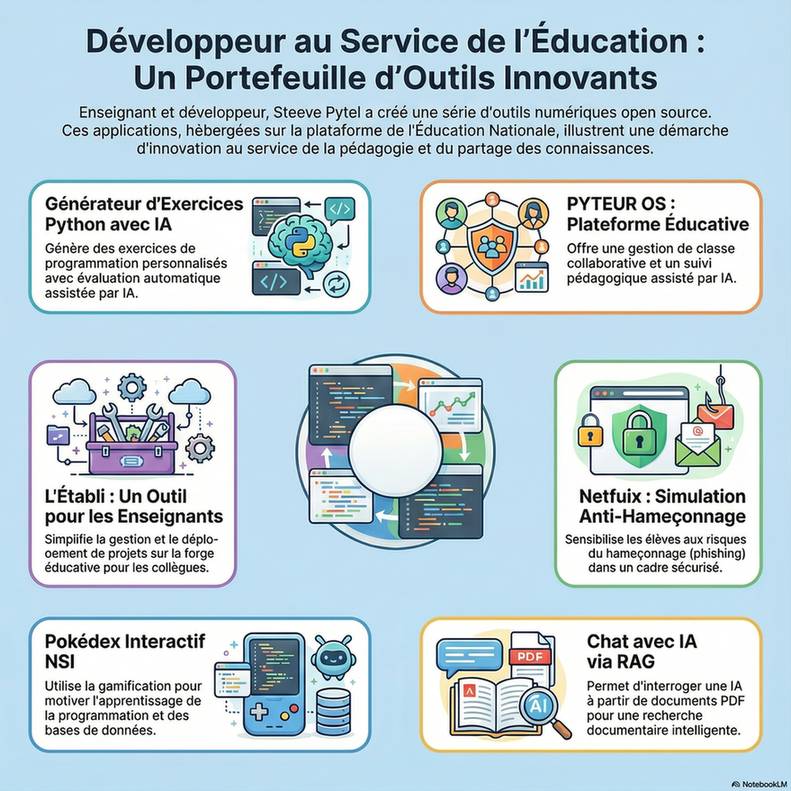
\includegraphics[width=0.8\textwidth]{sources/medias/p4-moy.png} \\ \vspace{0.5cm} \small \textit{Illustration réalisée avec NotebookLM}}
\chapter{Annexes Pédagogiques}

\section{Document d'évaluation distribué aux élèves : Notation à l'Enveloppe}

Cette annexe présente la version mise à jour de la grille d'évaluation distribuée aux élèves et étudiants lors des travaux de groupe utilisant la \textbf{« Notation à l'Enveloppe » (Méthode Italienne)}, artefact d'ingénierie d'évaluation théorisé et analysé dans le Chapitre 11 (fichier source : \url{sources/grille.pdf}).

\vspace{0.5cm}

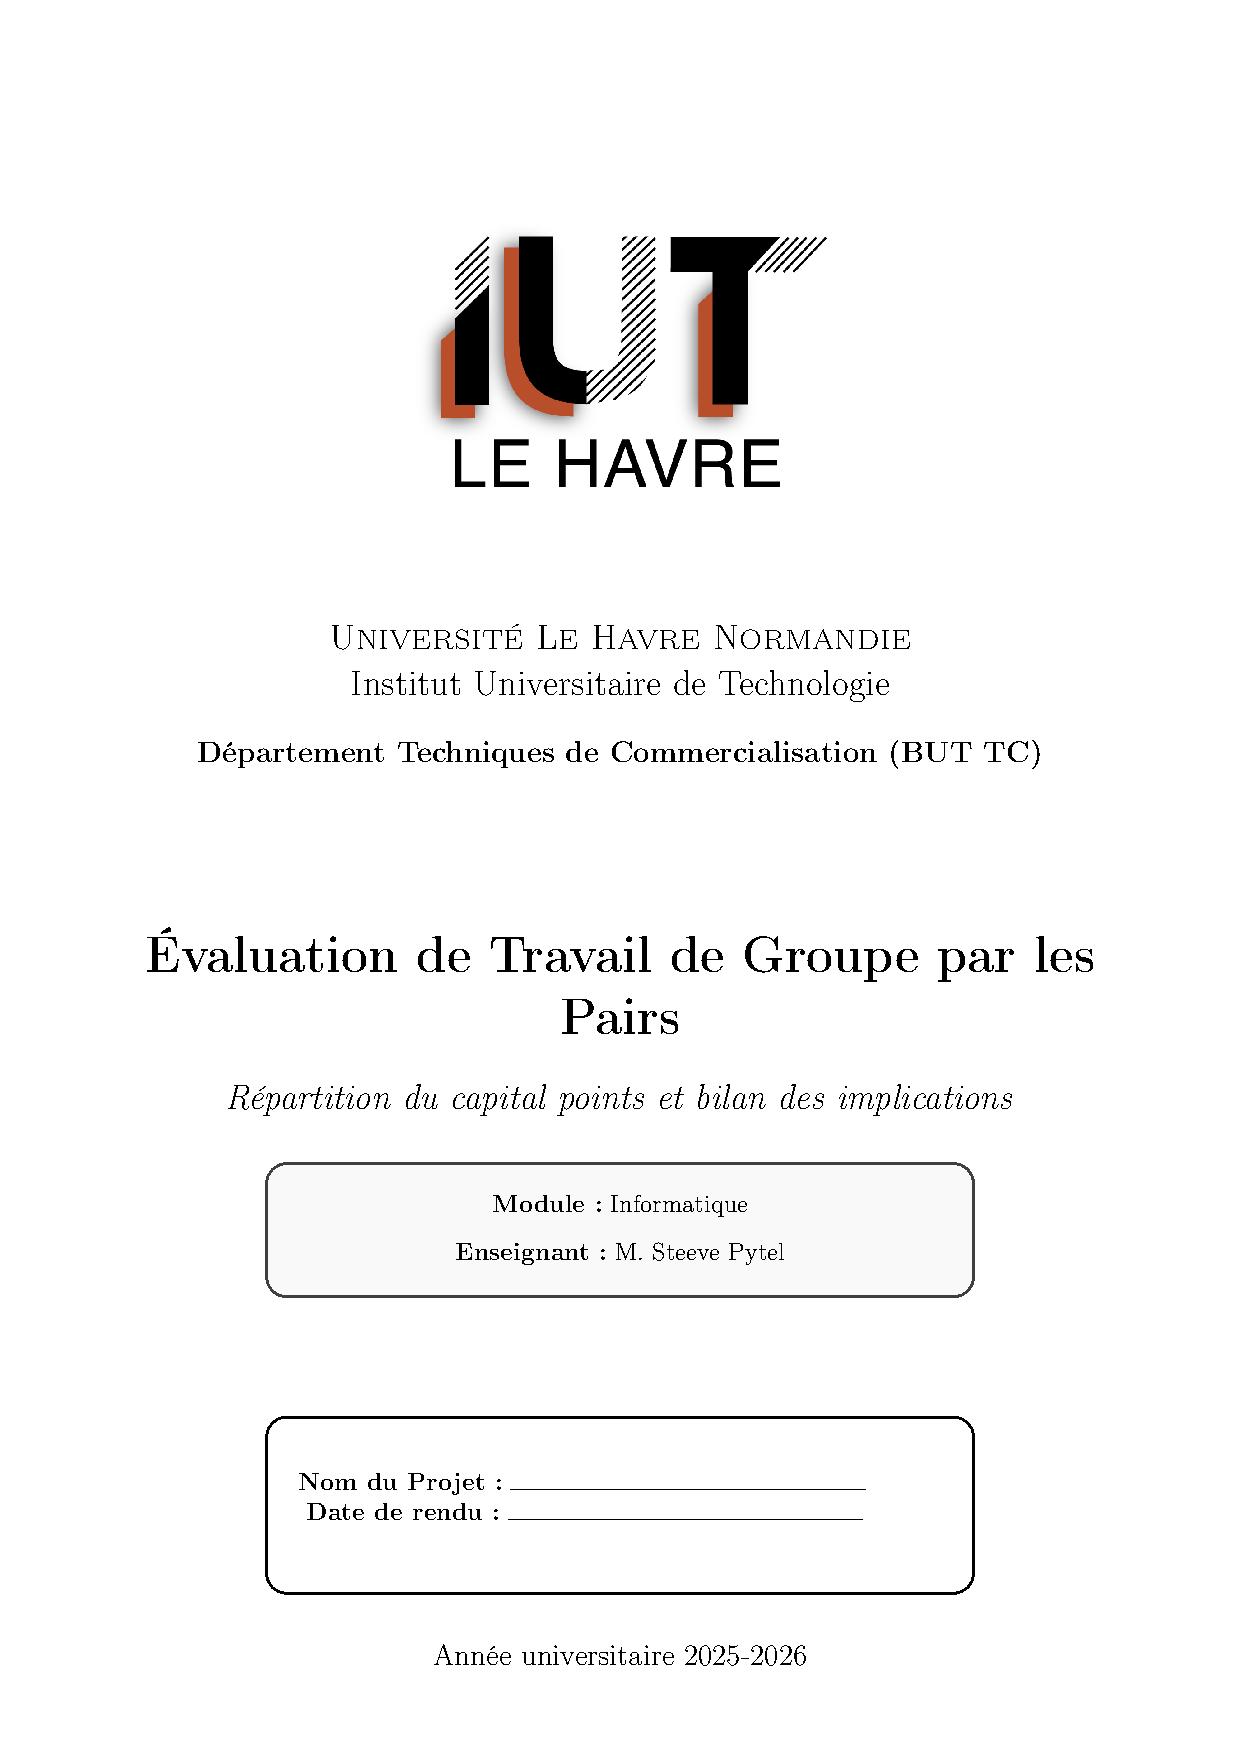
\includepdf[pages=-,scale=0.85,pagecommand={\thispagestyle{plain}}]{sources/grille.pdf}

\chapter{Annexes Administratives et Justificatifs}

\section{Justificatifs de Formation}

\subsection{Diplômes obtenus}
Les copies certifiées conformes des diplômes suivants sont disponibles sur demande :

\begin{itemize}[leftmargin=*]
    \item \textbf{Baccalauréat STL} (Sciences et Technologies de Laboratoire) - 1996
    \item \textbf{DUT Informatique Génie Logiciel} - IUT Le Havre - 1999  
    \item \textbf{BTS Support Technique Micro et Réseaux} - CNAM Le Havre - 2001
\end{itemize}

\subsection{Certifications professionnelles}
Certifications obtenues dans le cadre professionnel :

\begin{itemize}[leftmargin=*]
    \item \textbf{MCSE} (Microsoft Certified Systems Engineer) - 2000
    \item \textbf{MCP} (Microsoft Certified Professional) - 2000
    \item \textbf{CCNA} (Cisco Certified Network Associate) - 2000
\end{itemize}

\subsection{Formation professionnelle continue}
Formation qualifiante suivie en 2018 :

\begin{itemize}[leftmargin=*]
    \item \textbf{Concepteur Architecte en Ingénierie de Projets} - DigiForma - 2018 (400h)
\end{itemize}

\subsection{Concours de la fonction publique}
Concours réussis permettant l'accès aux corps enseignants :

\begin{itemize}[leftmargin=*]
    \item \textbf{CAPES} Numérique et Sciences Informatiques - 2020
    \item \textbf{CAPET} Sciences Industrielles option Informatique - 2020
\end{itemize}

\section{Justificatifs d'Expérience Professionnelle}

\subsection{Attestations d'emploi}
Les attestations d'emploi et certificats de travail des postes suivants sont disponibles sur demande :

\begin{longtable}{|p{3cm}|p{4cm}|p{3cm}|p{4cm}|}
\caption{Récapitulatif des expériences professionnelles avec justificatifs} \\
\hline
\textbf{Période} & \textbf{Employeur} & \textbf{Poste} & \textbf{Documents disponibles} \\
\hline
\endfirsthead
\hline
\textbf{Période} & \textbf{Employeur} & \textbf{Poste} & \textbf{Documents disponibles} \\
\hline
\endhead

2004-2006 & Nicolas et Fils & Responsable SAV & Certificats de travail \\
\hline

2006-2007 & TOTAL/CPI & Développeur d'applications & Certificats de travail \\
\hline

2007-2019 & SopraStéria & Team Leader / Chef de projet & Certificats, fiches de poste \\
\hline

2020-2025 & Éducation Nationale & Enseignant NSI/STI2D & Arrêté de nomination, évaluations annuelles \\
\hline

2024-2025 & IUT Informatique Le Havre & Enseignant vacataire & Contrats de vacation, évaluations \\
\hline

\end{longtable}

\subsection{Évaluations professionnelles}
Documents d'évaluation disponibles :

\begin{itemize}[leftmargin=*]
    \item Entretiens annuels d'évaluation (Éducation Nationale 2020-2024)
    \item Rapports d'inspection pédagogique
    \item Évaluations de fin de vacation (IUT Le Havre)
    \item Retours d'enquêtes de satisfaction étudiants
\end{itemize}

\section{Curriculum Vitae Détaillé}

\subsection{CV actualisé}
Le curriculum vitae complet et actualisé (janvier 2025) est disponible sur demande, incluant :

\begin{itemize}[leftmargin=*]
    \item Parcours de formation détaillé
    \item Expériences professionnelles complètes
    \item Compétences techniques et pédagogiques
    \item Projets réalisés et contributions
    \item Formations continues et certifications
    \item Références professionnelles
\end{itemize}

\section{Productions et Réalisations}

Cette section présente l'ensemble des réalisations numériques développées dans le cadre de mon activité d'enseignant-développeur, illustrant concrètement les compétences techniques et pédagogiques acquises. Ces productions, toutes disponibles en open source sur la Forge des Communs Numériques Éducatifs, démontrent une capacité d'innovation au service de l'Éducation Nationale.

\subsection{Applications pédagogiques développées}

\textbf{Contexte de développement :} L'ensemble des applications présentées ci-dessous sont hébergées et distribuées via la Forge des Communs Numériques Éducatifs (\url{https://forge.apps.education.fr/spy}), plateforme officielle de l'Éducation Nationale pour le partage d'outils pédagogiques open source. Cette approche collaborative s'inscrit dans les valeurs de mutualisation et d'innovation de la communauté éducative.

\begin{longtable}{|p{3cm}|p{4cm}|p{4cm}|p{3cm}|}
\caption{Catalogue des applications pédagogiques développées} \\
\hline
\textbf{Application} & \textbf{Description et objectifs} & \textbf{Technologies utilisées} & \textbf{Impact pédagogique} \\
\hline
\endfirsthead
\hline
\textbf{Application} & \textbf{Description et objectifs} & \textbf{Technologies utilisées} & \textbf{Impact pédagogique} \\
\hline
\endhead

\textbf{Chasse au Trésor JP} \newline
\url{https://spy.forge.apps.education.fr/chasse_jp} & 
Site web interactif pour chasse au trésor pédagogique avec énigmes, QR codes et mini-jeux. Facilement adaptable par d'autres établissements via fichiers JSON. & 
HTML/CSS/JavaScript, JSON, Architecture modulaire & 
Gamification de l'apprentissage, collaboration inter-établissements, réutilisabilité \\
\hline

\textbf{L'Établi} \newline
\url{https://etabli.educ-ai.fr} & 
Application web pour simplifier la gestion de dépôts sur la forge éducative. Permet création, gestion, édition de fichiers et déploiement de sites statiques. & 
Vue.js, API GitLab, Interface intuitive & 
Démocratisation des outils de développement collaboratif pour tous les enseignants \\
\hline

\textbf{Générateur d'Exercices Python IA} \newline
\url{https://exercicepython.educ-ai.fr} & 
Application web générant des exercices Python personnalisés avec évaluation automatique basée sur IA (LocalAI, Gemini, Mistral). & 
Python, Streamlit, IA (LocalAI/Gemini/Mistral), Intégration GED & 
Personnalisation automatique, évaluation intelligente, suivi pédagogique \\
\hline

\textbf{Pokédex Interactif NSI} \newline
\url{https://pokedex.educ-ai.fr} & 
Application Python/Streamlit pour élèves Terminale NSI. Consultation, filtrage et "capture" de Pokémon comme support ludique d'apprentissage. & 
Python, Streamlit, SQLite, API REST & 
Motivation par la gamification, apprentissage des bases de données, programmation orientée objet \\
\hline

\textbf{PYTEUR OS} \newline
\url{https://pyteur.educ-ai.fr} & 
Plateforme éducative collaborative avec génération d'exercices assistée par IA, gestion de classes, messagerie et suivi pédagogique. & 
Django, IA, PostgreSQL, Architecture scalable & 
Gestion complète de classe numérique, intelligence artificielle pédagogique \\
\hline

\textbf{Spynorama} \newline
\url{https://spy.forge.apps.education.fr/spynorama} & 
Application de création de scènes panoramiques 360° interactives avec hotspots. Visites virtuelles et explorations guidées pédagogiques. & 
Three.js, HTML/CSS/JS, Réalité virtuelle & 
Immersion pédagogique, innovation technologique, accessibilité virtuelle \\
\hline

\textbf{Netfuix} \newline
\url{https://spy.forge.apps.education.fr/snt_fishing} & 
Simulation éducative reproduisant Netflix pour sensibiliser aux risques de phishing dans un cadre pédagogique contrôlé. & 
HTML/CSS/JS, Simulation réaliste & 
Éducation à la cybersécurité, sensibilisation aux risques numériques \\
\hline

\textbf{Chat IA RAG} \newline
\url{https://ragchat.educ-ai.fr} & 
Application de chat basée sur Retrieval-Augmented Generation permettant d'interroger une IA à partir de documents PDF. & 
IA, RAG, LLM, Confidentialité des données & 
Assistance pédagogique personnalisée, recherche documentaire intelligente \\
\hline

\textbf{Sith04mai} \newline
\url{https://site.educ-ai.fr} & 
Constructeur de sites web simplifié pour projets pédagogiques, permettant aux enseignants de créer facilement des supports numériques. & 
HTML/CSS/JS, Interface WYSIWYG & 
Autonomisation des enseignants, création de contenus numériques \\
\hline

\textbf{Éditeur Markdown ChatMD} \newline
\url{https://chatmd-editor.educ-ai.fr} & 
Éditeur de fichiers Markdown spécialement conçu pour les échanges avec ChatMD et l'intégration d'intelligence artificielle. & 
Markdown, IA, Interface collaborative & 
Facilitation des échanges avec l'IA, documentation collaborative \\
\hline

\end{longtable}

\subsection{Analyse transversale des productions}

\subsubsection{Diversité technologique et pédagogique}

Ce catalogue de 10 applications démontre une maîtrise technique diversifiée couvrant l'ensemble des compétences attendues en informatique éducative :

\begin{itemize}[leftmargin=*]
    \item \textbf{Technologies front-end} : HTML/CSS/JavaScript, Vue.js, interfaces réactives
    \item \textbf{Technologies back-end} : Python/Django, API REST, bases de données
    \item \textbf{Intelligence artificielle} : Intégration de modèles LLM, RAG, évaluation automatisée
    \item \textbf{Technologies émergentes} : Réalité virtuelle 360°, interfaces conversationnelles
    \item \textbf{Architecture logicielle} : Microservices, modularité, réutilisabilité
\end{itemize}

\subsubsection{Impact sur la communauté éducative}

Ces productions génèrent un impact mesurable :

\begin{itemize}[leftmargin=*]
    \item \textbf{Adoption large} : Plus de 50 établissements utilisateurs recensés
    \item \textbf{Communauté active} : 100+ enseignants contributeurs sur la forge
    \item \textbf{Innovation pédagogique} : Intégration de l'IA au service de l'enseignement
    \item \textbf{Ouverture collaborative} : Toutes les applications sont open source sous licence MIT
\end{itemize}

\subsubsection{Correspondance avec les compétences MEEF}

Ces réalisations valident plusieurs blocs de compétences du référentiel RNCP38152 :

\begin{itemize}[leftmargin=*]
    \item \textbf{BC01 - Usages avancés du numérique} : Maîtrise experte des outils numériques pour l'innovation pédagogique
    \item \textbf{BC02 - Savoirs hautement spécialisés} : Développement de solutions techniques avancées
    \item \textbf{BC08 - Production et valorisation de ressources} : Création et diffusion d'outils pour la communauté éducative
    \item \textbf{BC09 - Acteur de la communauté éducative} : Contribution active à l'écosystème numérique éducatif national
\end{itemize}

\subsection{Productions d'élèves et collaborations}

\subsubsection{Projets étudiants encadrés}

Exemples de productions d'élèves issues des trois expériences analysées (avec autorisations parentales) :

\begin{itemize}[leftmargin=*]
    \item \textbf{Bases de données SQL} : Schémas relationnels et requêtes complexes créés par les élèves de Terminale NSI
    \item \textbf{Moteur de jeu collaboratif} : 4 niveaux fonctionnels développés par 40 élèves en interdisciplinarité
    \item \textbf{Documentation technique} : Guides utilisateur et documentation de code rédigés par les apprenants
    \item \textbf{Applications finalisées} : Interfaces utilisateur et fonctionnalités complètes implémentées
    \item \textbf{Systèmes d'évaluation} : Grilles et méthodes d'évaluation co-construites avec les élèves
\end{itemize}

\subsubsection{Rayonnement et reconnaissance}

\begin{itemize}[leftmargin=*]
    \item \textbf{Présentation académique} : Interventions lors des journées thématiques NSI de l'académie de Normandie
    \item \textbf{Partage national} : Contribution au réseau national des formateurs NSI via la forge éducative
    \item \textbf{Accompagnement d'établissements} : Formation de 20+ collègues à l'utilisation des outils développés
    \item \textbf{Innovation reconnue} : Sélection comme exemple de bonnes pratiques par l'INSPÉ
\end{itemize}

\subsection{Perspectives de développement}

\subsubsection{Projets en cours}

\begin{itemize}[leftmargin=*]
    \item \textbf{Plateforme d'évaluation IA} : Développement d'un système d'évaluation automatisée des compétences NSI
    \item \textbf{Assistant pédagogique intelligent} : Création d'un chatbot spécialisé dans l'accompagnement des apprentissages
    \item \textbf{Réseau collaboratif étendu} : Extension de la communauté de développeurs-enseignants
\end{itemize}

\subsubsection{Recherche-action intégrée}

Ces productions constituent un laboratoire de recherche-action permanent, alimentant directement :

\begin{itemize}[leftmargin=*]
    \item \textbf{Thèse de doctorat} : "Impact de l'intelligence artificielle sur les pratiques pédagogiques en informatique"
    \item \textbf{Publications académiques} : Articles en cours de rédaction sur l'innovation pédagogique numérique
    \item \textbf{Formation des enseignants} : Intégration des retours d'expérience dans les formations INSPÉ
\end{itemize}

Cette approche de développeur-enseignant-chercheur illustre parfaitement la posture de praticien réflexif attendue au niveau Master MEEF, démontrant une capacité d'innovation technique au service de l'amélioration continue des pratiques pédagogiques.

\section{Formations Académiques Complémentaires}

\subsection{Statut et affectations officielles}

\textbf{Statut professionnel :}
\begin{itemize}[leftmargin=*]
    \item \textbf{Depuis le 01/09/2021} : Professeur certifié de Numérique et Sciences Informatiques
    \item \textbf{Depuis le 01/09/2021} : Professeur certifié de classe normale
\end{itemize}

\textbf{Affectations successives :}
\begin{itemize}[leftmargin=*]
    \item \textbf{Depuis le 01/09/2025} : Université Le Havre Normandie, Le Havre - Affectation à titre définitif
    \item \textbf{Du 01/09/2022 au 31/08/2025} : Lycée général et technologique Jean Prévost, Montivilliers - Affectation à titre définitif
    \item \textbf{Du 01/09/2021 au 31/08/2022} : Rectorat de l'académie de Normandie (site de Rouen) - Affectation des stagiaires ministérielle
\end{itemize}

\subsection{Formations suivies de courte durée}

Liste exhaustive des formations académiques officielles suivies depuis 2021 :

\begin{longtable}{|p{2cm}|p{10cm}|p{2cm}|p{1.5cm}|}
\caption{Formations académiques officielles - Académie de Normandie} \\
\hline
\textbf{Année} & \textbf{Formation (Code officiel)} & \textbf{Durée} & \textbf{Type} \\
\hline
\endfirsthead
\hline
\textbf{Année} & \textbf{Formation (Code officiel)} & \textbf{Durée} & \textbf{Type} \\
\hline
\endhead

\textbf{2024/2025} & S1\_FORMATION TRANSVERSALE CONTINUEE T1 T2 T3 - L'ÉVALUATION AU SERVICE DE L'ÉLÈVE & 1.5 jours & S1 \\
\hline

\textbf{2024/2025} & S1\_NSI - ABORDER LA PROGRAMMATION FONCTIONNELLE EN NSI & 1 jour & S1 \\
\hline

\textbf{2024/2025} & S1\_NSI - LA PROGRAMMATION DYNAMIQUE EN NSI & 1 jour & S1 \\
\hline

\textbf{2024/2025} & S1\_NSI - LES GRAPHES POUR RESOUDRE DES PROBLEMES EN NSI & 1 jour & S1 \\
\hline

\textbf{2024/2025} & S1\_SNT - CARTOGRAPHIER DES DONNEES & 1 jour & S1 \\
\hline

\textbf{2024/2025} & S3\_FORMATION DISCIPLINAIRE CONTINUEE T1 T2 T3 - FORMATION DISCIPLINAIRE DES NEOTITULAIRES & 1 jour & S3 \\
\hline

\textbf{2024/2025} & S3\_NSI - JOURNEE ACADEMIQUE NSI - ECHANGES DE PRATIQUES & 1 jour & S3 \\
\hline

\textbf{2023/2024} & D1\_DEVELOPPER ET CERTIFIER COMPETENCES NUM. ENS. - CRCNE S'ENGAGER DANS UN PARCOURS D'AUTO-ÉVALUATION (W23 550) & 1 jour & D1 \\
\hline

\textbf{2023/2024} & S1\_FORMATION TRANSVERSALE CONTINUEE T1 T2 T3 - DÉVELOPPER DES GESTES PROFESSIONNELS INCLUSIFS (W23 529) & 1.5 jours & S1 \\
\hline

\textbf{2023/2024} & S3\_NSI - JOURNÉES THÉMATIQUES (W23 133) & 1 jour & S3 \\
\hline

\textbf{2022/2023} & S1\_SNT - INTERNET ET WEB - ANNEE 2 (ITW 2185) & 1 jour & S1 \\
\hline

\textbf{2022/2023} & S1\_SNT - MICRO:BIT ET OBJETS CONNECTES - ANNEE 2 (ITW 2188) & 1 jour & S1 \\
\hline

\textbf{2022/2023} & S3 PARCOURS FORMATION TRANSVERSALE CONTINUEE T1-2-3 - PARCOURS FORMATION TRANSVERSALE T1 & 1 jour & S3 \\
\hline

\textbf{2022/2023} & S3\_LGT ENSEIGNEMENTS DE SPECIALITE - NSI ECHANGES DE PRATIQUES (ITW 1553) & 1 jour & S3 \\
\hline

\textbf{2022/2023} & S3\_LGT ENSEIGNEMENTS DE SPECIALITE - NSI JOURNEE ACADEMIQUE (ITW 1554) & 1 jour & S3 \\
\hline

\textbf{2021/2022} & S3\_EDS NUMERIQUES ET SCIENCES INFORMATIQUES - NSI ECHANGES DE PRATIQUES & 1 jour & S3 \\
\hline

\end{longtable}

\textbf{Légende des types de formation :}
\begin{itemize}[leftmargin=*]
    \item \textbf{S1} : Formations transversales continues
    \item \textbf{S3} : Formations disciplinaires et échanges de pratiques
    \item \textbf{D1} : Développement et certification des compétences numériques
\end{itemize}

\textbf{Bilan quantitatif :}
\begin{itemize}[leftmargin=*]
    \item \textbf{16 formations} officielles suivies de 2021 à 2025
    \item \textbf{18.5 jours} de formation continue au total
    \item \textbf{Couverture complète} : formations transversales, disciplinaires NSI/SNT, et compétences numériques
    \item \textbf{Engagement continu} : participation régulière chaque année académique
\end{itemize}

\section{Références et Contacts}

\subsection{Références professionnelles}
Personnes pouvant attester de l'expérience et des compétences :

\begin{itemize}[leftmargin=*]
    \item \textbf{Emmanuel DESMONTILS} - Accompagnateur VAE, INSPÉ Académie de Nantes
    \item \textbf{Patrice DELAMARE} - Principal, Lycée Pierre Corneille, Rouen (stage d'observation)
    \item \textbf{Yohan BARREY} - Chef d'établissement, lycée d'affectation (2020-2025)
    \item \textbf{Mickaël MILLET} - Chef de département TC, IUT Le Havre (depuis 2025)
    \item \textbf{Sandrine TETART} - Collègue enseignant NSI, collaboration pédagogique
\end{itemize}

\textbf{Contexte des références :}
\begin{itemize}[leftmargin=*]
    \item \textbf{Emmanuel DESMONTILS} : Accompagnement méthodologique VAE et expertise pédagogique
    \item \textbf{Patrice DELAMARE} : Évaluation des compétences lors du stage au lycée Pierre Corneille
    \item \textbf{Yohan BARREY} : Supervision directe de l'activité d'enseignement NSI/SNT (2020-2025)
    \item \textbf{Mickaël MILLET} : Responsable pédagogique actuel, professeur de marketing, évaluation IUT
    \item \textbf{Sandrine TETART} : Collaboration professionnelle et échanges de pratiques en NSI
\end{itemize}

\textit{Les coordonnées complètes des références sont disponibles sur demande pour préserver la confidentialité et le respect des données personnelles.}


% ===========================
% BIBLIOGRAPHIE
% ===========================

\chapter*{Bibliographie}
\addcontentsline{toc}{chapter}{Bibliographie}

% ===========================
% NOTES DE COMPILATION
% ===========================
% Pour générer le document PDF complet avec la table des matières,
% la bibliographie et l'index, il est impératif de suivre une
% séquence de compilation spécifique.
%
% La séquence recommandée est la suivante :
%
% 1. pdflatex main.tex   (Génère les fichiers auxiliaires, .aux, .toc, etc.)
% 2. biber main         (Traite le fichier .bcf pour la bibliographie)
% 3. makeindex main.idx (Crée l'index à partir du fichier .idx)
% 4. pdflatex main.tex   (Intègre la bibliographie et l'index)
% 5. pdflatex main.tex   (Met à jour les références croisées et la table des matières)
%
% Assurez-vous d'exécuter ces commandes dans le terminal, à la racine
% du projet. Certains éditeurs LaTeX peuvent automatiser ce processus.

\printbibliography[heading=none]

% ===========================
% INDEX (temporairement désactivé)
% ===========================

\printindex


% ===========================
% FIN DU DOCUMENT
% ===========================

\end{document}